\documentclass[archive]{mgr}

\usepackage{polski}
\usepackage[utf8]{inputenc}
\usepackage[T1]{fontenc}
\usepackage{indentfirst}

\usepackage{graphicx}
\usepackage{subfigure}
\usepackage{psfrag}

\usepackage{amsmath}
\usepackage{amsfonts}
\usepackage{textcomp}
\usepackage{supertabular}
\usepackage{array}
\usepackage{tabularx}
\usepackage{hhline}
\usepackage{url}
\usepackage{listings}


\newcommand{\R}{I\!\!R}
\newtheorem{theorem}{Twierdzenie}[section]

\title{Analiza porównawcza wybranych implementacji API OpenGL i DirectX}
\engtitle{Comparison analysis of selected implementations of OpenGL and DirectX APIs}
\author{ Wojciech Urbańczyk}
\supervisor{dr inż. Jarosław Rudy, K30W04D03}
\field{Informatyka (INF)}
\specialisation{Inżynieria systemów informatycznych (INS)}

\renewcommand{\lstlistlistingname}{Spis listingów}

\begin{document}
\bibliographystyle{plabbrv}

\maketitle

\tableofcontents

\listoffigures
\listoftables
\lstlistoflistings

\chapter{Wstęp}


 Moc obliczeniowa kolejnych generacji układów graficznych nieustannie rośnie podążają za rosnącym zapotrzebowaniem. Popyt ten jest generowany głównie przez branżę gier komputerowych, koparki krypto–walut i zastosowania naukowe, inżynierskie i biznesowe. Równolegle z rozwojem sprzętu ulepszane jest oprogramowanie z nim związane. Na przestrzeni lat pojawiały się różne rozwiązania, część z nich dla specyficznych problemów, a inne obierały bardziej uniwersalne podejście. Obecnie na rynku istnieje wiele rodzajów oprogramowania służącego do sterowania kartami graficznymi. Najbardziej rozpowszechnionymi, szczególnie na rynku gier, są API DirectX i OpenGL, a o ich dominacji zadecydowało wiele czynników. Każdy z nich ma swoje mocne i słabe strony i nie można jednoznaczne stwierdzić, który z nich jest lepszy. Jednak poprzez zrozumie różnic pomiędzy nimi jest możliwe, aby określić, który z nich jest lepszy do konkretnego zastosowania. \\
 
Podczas badań skupiono się na różnych zmiennych, które mogą determinować wydajność interfejsu. Jednym z takich elementów jest producent, model i generacja karty graficznej. Raz napisane oprogramowanie graficzne powinno być kompatybilne z jak największą liczbą komputerów i systemów operacyjnych. Z tego powodu każde zaplanowane badanie wykonano dla trzech układów graficznych. Pomogło to określić czy oprogramowanie skierowane na konkretną kartę graficzną będzie działało w odpowiedni sposób. Każdy z wykonanych testów pozwolił na wyciągnięcie pewnych wniosków i~poszerzenie wiedzy. Dzięki temu twórca oprogramowania wyposażony w te informacje jest w stanie opracowywać lepsze rozwiązania i budować wydajniejsze programy.\\

Celem pracy jest porównanie wydajności interfejsów OpenGL oraz DirectX (m.in. pomiar czasu renderowania sceny) przy różnych parametrach sceny. W pierwszej kolejności należy przeprowadzić studia literaturowe, które pozwolą określić co w tej dziedzinie już wykonano i jakimi metodami się posłużono. Kolejnym celem jest stworzenie silnika graficznego umożliwiającego definiowanie i renderowanie scen 3D z użyciem podstawowych mechanizmów typu teksturowanie czy oświetlanie sceny z użyciem modelu Phonga. Silnik będzie umożliwiał wybór cech takich jak liczba i położenie obiektów (wielokątów, źródeł światła, użytej tekstury itp.). Silnik będzie wspierał renderowanie sceny przy pomocy API OpenGL oraz DirectX. Następnie należy zaplanować badania. Przygotowane zostaną przykładowe scenariusze testowe, które posłużą do przeprowadzenia badań. Na ich podstawie i z użyciem narzędzi badawczych zostaną wykonane pomiary. Otrzymane wyniki zostaną poddane analizie oraz porównane z wynikami dostępnymi w literaturze.
\newpage

W pracy pokazano różnice pomiędzy API OpenGL oraz DirectX na różnych polach. W drugim rozdziale przedstawiono ich cechy pod kątem ich cyklu rozwoju, dostępności, przenośności czy łatwości w implementacji własnych rozwiązań. Wszystkie te atrybuty zostały porównane ze swoimi odpowiednikami w drugim API, tak aby otrzymać spójny obraz obu interfejsów i różnic pomiędzy nimi. Dalsza część pracy skupia się na własności, którą można określi tylko poprzez wykonanie odpowiednich badań – wydajności. Najpierw należało określić co w tej dziedzinie zostało już zrobione, jakimi podejściami i z jakimi rezultatami. W rozdziale 3 wykonano przegląd literatury pozwolił na zebranie dostępnej wiedzy i użycie jej jako punktu wyjścia. Na jej podstawie z użyciem różnych narzędzi badawczym, w tym z autorskim silnik graficznym wykonano pomiary w pewnych założonych wcześniej warunkach. Pozwoliło to na zebranie dużej ilości danych, które po stosownej obróbce statystycznej zostały poddane analizie. Etap ten przedstawiono w rozdziale 4, który zawiera plan badań, opis środowiska badawczego, analizę wyników oraz podsumowanie. Ostatnim rozdziałem pracy jest zakończenie, w którym pokazano co z pośród postawionych celów zostało wykonane i z jakim rezultatem.





\chapter{API graficzne}

Celem tego rozdziału jest przybliżenie sposobu działania interfejsów programowania aplikacji (ang. Application Programming Interface, API) OpenGL i DirectX i analiza elementów z których się składają. Pierwsze dwie sekcje skupiają się na opisie pewnych kluczowych aspektów związanych z tymi interfejsami, takich jak sposób rozwoju standardu, metody przesyłu danych czy potok graficzny,a w szczególności jego programowalna część. W dalszej części rozdziału dokonano porównania omówionych elementów i wyszczególniono spostrzeżone różnice oraz podobieństwa.

\section{OpenGL}

OpenGL to interfejs programowania aplikacji, którego głównym celem jest ułatwienie interakcji z procesorem graficznym (ang. Graphics Processing Unit, GPU). Najczęściej jest wykorzystywany do renderowania grafiki wektorowej 2D i 3D, ale ze względu na możliwości kart graficznych do realizowania wielu zadań jednocześnie bywa także stosowany do wykonywania zadań obliczeniowych. Początkowo rozwijany przez Silicon Graphics, Inc. (SGI) i wydany w 1992 roku OpenGL miał oddzielić warstwę sprzętową od programowej tak, aby programiści mogli tworzyć oprogramowanie działające niezależnie od sprzętu na którym zostanie uruchomione. Od 2006 roku opiekę nad standardem sprawuje konsorcjum Khronos Group. Obecnie najnowszą wersją API jest ta oznaczona numerem 4.6 ogłoszona w 2017 rok \cite{OpenGLHistory}. W pracy została wykorzystana najnowsza w momencie pisania wersja  4.6.\\

Cechą charakterystyczną OpenGL jest to w jaki sposób jest rozwijany. Wprowadzone zostało pojęcie rozszerzeń (ang.  extensions), które oznacza nowe lub rozszerzone funkcje API, które nie są zawarte w głównej specyfikacji OpenGL. Producenci kart graficznych oraz sterowników mogą dodawać własne funkcjonalności do implementacji interfejsu. Jeżeli zaproponowane rozszerzenie jest powszechnie stosowane przez wielu producentów, to może zostać dodane do głównego standardu, co oznacza, że każda implementacja jest zobowiązana posiadać tę funkcjonalność. Cześć rozszerzeń może być dostępna tylko dla konkretnych modeli kart graficznych, dlatego OpenGL posiada mechanizmy, które pozwalają czy rozszerzenie jest dostępne na konkretnej stacji. Rozszerzenie należą do 3 grup:
\begin{itemize}
  \item generyczne,
  \item zatwierdzone przez Architecture Review Board (ARB),
  \item specyficzne dla danego producenta.
\end{itemize}
\newpage
Rozszerzenia generyczne mogą być implementowane przez wiele sterowników i nie są przypisanego do jednego producenta. Takie rozszerzenie może zostać zatwierdzone przez ARB, co oznacza, że prawdopodobnie zostanie dodane do standardu. Każde rozszerzenie posiada prefiks, na podstawie którego można określić do której grupy należy. W tabeli \ref{OpenGLExtensionsTable} przedstawiono prefiksy używane przez różnych producentów oprogramowania graficznego \cite{OpenGLExtensions}. 
\begin{table}[]

    \centering % instead of \begin{center}
    \caption{Prefiksy rozszerzeń OpenGL}
    		\label{OpenGLExtensionsTable}
    \vspace{2mm} % Adjust the height of the space between caption and tabular
\begin{tabular}{|l|l|}
\hline
\textbf{Prefiks rozszerzenia} & \textbf{Typ, producent lub platforma} \\ \hline
ARB                           & Zatwierdzone przez ARB                \\ \hline
GL\_EXT                       &Generyczne                            \\ \hline
NV	& NVIDIA Corporation.\\ \hline
ATI	& ATI Technologies, Inc.\\ \hline
3DLABS	& 3DLABS, Inc.\\ \hline
SUN	& Sun Microsystems, Inc.\\ \hline
SGI	& Silicon Graphics, Inc.\\ \hline
SGIX &	Silicon Graphics, Inc. Experimental extension.1\\ \hline
SGIS &	Silicon Graphics, Inc. Experimental extension.1\\ \hline
INTEL &	Intel Corporation.\\ \hline
3DFX &	3dfx Interactive.\\ \hline
IBM &	International Business Machines Corporation\\ \hline
MESA &	Biblioteka graficzna Mesa 3D\\ \hline
GREMEDY &	Graphic Remedy, Ltd.\\ \hline
OML &	Khronos Group, Inc. API: OpenML®\\ \hline
OES &	Khronos Group, Inc. API: OpenGL® ES\\ \hline
PGI &	Portland Group Inc.\\ \hline
I3D &	Intense3D, now 3DLABS Inc.\\ \hline
INGR &	Intergraph Corporation.\\ \hline
MTX &	Matrox Electronic Systems Ltd.\\ \hline
WGL\_EXT, WGL\_ARB &	Microsoft Corporation. WGL = Windows OpenGL\\ \hline
GLX\_EXT, GLX\_ARB &	X–Window\\ \hline
AGL &	Apple Inc. AGL = Apple OpenGL\\ \hline
\end{tabular}
\end{table}
Do wersji 2.1. OpenGL działał w tzw. trybie natychmiastowym. Polegał on na tym, że dane wymagane do zbudowania sceny (np. współrzędne wierzchołków, współrzędne tekstur, wektory normalne, kolor) były przesyłane do GPU przez procesor (ang. central processing unit, CPU) w każdej klatce. Skutkowało to tym, że gdy scena ulegała niewielkiej zmienia np. obrót obiektu, wszystkie dane musiały być przesyłane jeszcze raz. Wraz ze wzrostem wymagań co do jakości renderowanej grafiki jak i rozwojem rynku gier komputerowych to podejście musiało ulec zmianie. Rozwiązaniem okazały się programowalne potoki graficzne, które stały się częścią standardu od wersji 3.0. Dzięki nim możliwe jest przesłanie dużej ilości danych do pamięci karty graficznej jednokrotnie przed rozpoczęciem rysowania, a następnie jedynie przekształcanie tych danych (np. obrót obiektu poprzez pomnożenie wierzchołków przez macierz przekształcenia liniowego). 
Miejsce, w~którym te dane są przetrzymywane określa się mianem bufora wierzchołków (ang. vertex buffer), a~programy wykonujące operacje na tych danych przy użyciu zasobów procesora graficznego modułami lub programami cieniującymi (ang. shader) \cite{kiciak}.
\newpage
Przed przystąpieniem do procesu renderowania należy w odpowiedni sposób przygotować dane. Informacje o parametrach wierzchołków są przekazywane w tablicy, chodź ułożenie tych danych może być różne. Programista musi poinformować sterownik w jaki sposób zorganizowane są dane. Realizowane jest to przy użyciu polecenia \emph{glVertexAttribPointer}, które przedstawiono na listingu \ref{glVertexAttribPointer} \cite{OpenGLAttrib}.\\

\begin{lstlisting}[caption={Funkcja glVertexAttribPointer},captionpos=b,label={glVertexAttribPointer}]
 void glVertexAttribPointer(	GLuint index,
 	GLint size,
 	GLenum type,
 	GLboolean normalized,
 	GLsizei stride,
 	const void * pointer);
\end{lstlisting}

Dane, które są stałe dla każdego wierzchołka są przekazywane do obiektów zwanych uniformami. Na listingu \ref{lab:primitives} pokazano shader, który zawiera uniform dla macierzy przekształcenia MVP (ang. Model View Projection). To w jaki sposób dane to są wysyłane do karty graficznej jest zależne od użytego języka. Przed wysłaniem danych należy najpierw pobrać lokację uniformu. Przykład dla języka C++ przedstawiono na listingu \ref{lab:uniform}.
\\


\begin{lstlisting}[caption={Ustawianie wartości uniformu w języku C++},captionpos=b,label={lab:uniform}]
GLint loc = glGetUniformLocation(ProgramObject, "Scale");
if (loc != -1)
{
   glUniform1f(loc, 0.432);
}
\end{lstlisting}

Odpowiednio przygotowana tablica z parametrami wierzchołków jest kopiowana do~pamięci karty graficznej reprezentowanej przez obiekt bufora wierzchołków (ang. \emph{Vertex Buffer Object, VBO)}. Następnie tak stworzony Vertex Buffer Object należy przypiąć do obiektu tablicy wierzchołków (ang. \emph{Vertex Array Object, VAO)}, który przetrzymuje informacje o~lokalizacji danych w pamięci oraz ich strukturze. Na listingu \ref{lab:vao} przykład kodu realizującego taki scenariusz dla języka C++ \cite{VertexSpecification}.\\


\begin{lstlisting}[caption={Definiowanie właściowści VAO},captionpos=b,label={lab:vao}]
glBindBuffer(GL_ARRAY_BUFFER, buf1);
glVertexAttribPointer(0, 4, GL_FLOAT, GL_FALSE, 0, 0);
glBindBuffer(GL_ARRAY_BUFFER, 0);
\end{lstlisting}


Pierwszym zadaniem potoku jest przetworzenie wejściowych wierzchołków w shaderze wierzchołków (ang. \emph{Vertex Shader}) \cite{OpenGLVertexShader}. Każdy wierzchołek wejściowy jest poddawany pewnym transformacją i zwracanym jako wierzchołek wyjściowy. Ważne by zaznaczyć, że możliwe jest także przetworzenie i zwrócenie innych danych (np. zmiana koloru wierzchołka na podstawie jego położenia), dzięki czemu na kolejnych etapach możliwe jest wykorzystanie wcześniej przygotowanych danych. Dla API OpenGL wszystkie shadery są pisane w języku \emph{OpenGL Shading Language (GLSL)}. Na listingu \ref{lab:vertexshader} przedstawiono kod przykładowego shadera wierzchołków. Jego zadaniem jest przekształcenie wierzchołków na podstawie macierzy MVP oraz przekazanie danych do dalszych etapów potoku. Warto zwrócić uwagę na pierwszą linijkę kodu, która definiuje wersję języka. Następnie znajdują się definicje parametrów wejściowych i wyjściowych oraz wykonywana funkcja \emph{main}. 
 Przetworzona pozycja wierzchołków jest wpisywana do zmiennej \emph{gl\_position}.

Kolejne dwa etapy polegają na pewnych przekształceniach wierzchołków w grupy zwane prymitywami (ang. primitives) i są niezbędnym elementem potoku. Reprezentują one pewne kształty, które z wizualizowano na rysunku \ref{lab:primitives} \cite{OpenGLPrimitives}.
\begin{figure}[h!]
  \centering
    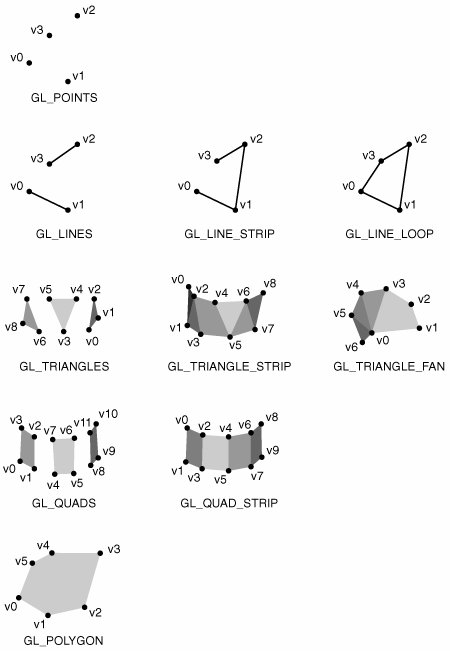
\includegraphics[width=0.50\textwidth]{images/primitives.jpg}
   \caption{Prymitywy OpenGL}
   Źródło: [https://flylib.com/books/2/789/1/html/2/images/02fig01.jpg]
   \label{lab:primitives}
\end{figure}
\begin{lstlisting}[caption={Kod shadera wierzchołków},captionpos=b,label={lab:vertexshader}]
#version 400 core
in vec4 in_Position;
in vec4 in_Color;  
in vec4 in_Normal;
out vec3 pass_Normal;
out vec3 pass_Color;
uniform mat4 MVP_Matrix;
void main(void) {
	gl_Position = MVP_Matrix * in_Position;
	pass_Color = in_Color.xyz;
	pass_Normal = in_Normal.xyz;

}
\end{lstlisting}
\newpage
Tak zgrupowane wierzchołki są przekazywane do shadera geometrii (ang. \emph{Geometry Shader}). Ma on dostęp do wszystkich wierzchołków danego prymitywa, dzięki czemu pozwala on na zmianę geometrii, albo dynamiczne obliczanie wektorów normalnych. Jest to etap programowalny, przez co programista ma pełną kontrolę nad tym procesem.\\

Kolejne trzy etapy (Vertex Post–Processing, Primitive Assembly, Rasterization) są stałe, a zmiana sposobu ich działania jest możliwa w ograniczonym stopniu poprzez ustawianie flag. W tych krokach wierzchołki są poddawana obcinaniu i pewnym transformacją, następnie są łączone w prymitywy bazowe oraz poddawane rasteryzacji, czyli procesowi podziału prymitywów na fragmenty. Ilość fragmentów, odpowiadających jednemu pikselowi na ekranie jest zależna od ustawionej opcji antyaliasingu (Rysunek \ref{lab:antyaliasing}). Opcją tą można sterować używając flagi \emph{GL\_MULTISAMPLE}(Listing \ref{lab:multisample}).

\begin{figure}[h!]
  \centering
    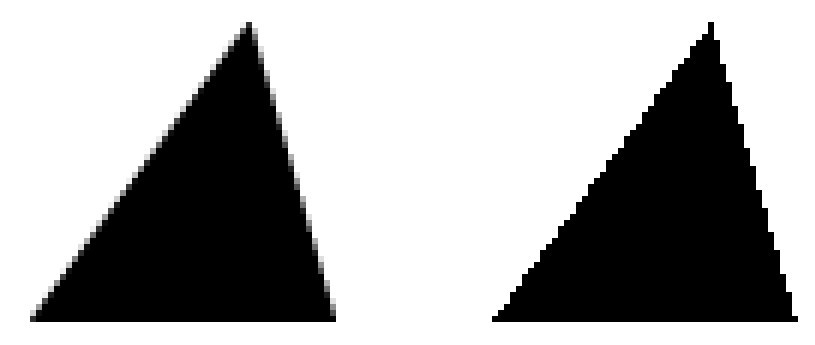
\includegraphics[width=0.30\textwidth]{images/antyaliasing.png}
   \caption{Przykład antyaliasingu}
   \label{lab:antyaliasing}
\end{figure}

\begin{lstlisting}[caption={Włączenie antyaliasingu OpenGL},captionpos=b,label={lab:multisample}]
glEnable(GL_MULTISAMPLE);  
\end{lstlisting}

\begin{figure}[h!]
  \centering
    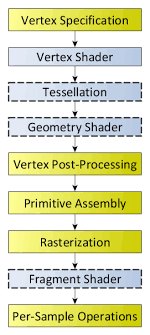
\includegraphics[width=0.30\textwidth]{images/RenderingPipeline.png}
   \caption{Diagram potoku graficznego dla OpenGL}
   Źródło: [https://www.khronos.org/opengl/wiki\_opengl/images/RenderingPipeline.png]
   \label{lab:pipeline}
\end{figure}
\newpage
Przedostatnim elementem potoku jest programowalny shader fragentów (ang. Fragment Shader). Jest on wykonywany dla każdego fragmentu stworzonego w procesie rasteryzacji. Na tym etapie programista może samodzielnie definiować w jaki sposób jest obliczany kolor konkretnego fragmentu. W tym shaderze najczęściej implementowane są takie elekty jak np. oświetlenie. Tak jak w przypadku shadera wierzchołków kod napisany został w języku GLSL (Listing \ref{lab:fragmentshader}).\\

Ostatni etap jest stały i polega na przetworzeniu wyjściowych fragmentów z poprzedniego kroku za pomocą operacji takich jak \emph{Scissor Test}, \emph{Stencil Test}, \emph{Depth Test} czy  \emph{Blending}. Pełen potok graficzny przedstawiono na Rysunku \ref{lab:pipeline}    \cite{Rendering_Pipeline_Overview}, gdzie kolorem niebieskim zaznaczone etapy programowalne.

\begin{lstlisting}[caption={Shader fragmentów, oświetlenie według modelu Phonga},captionpos=b,label={lab:fragmentshader}]
#version 400 core
in vec3 pass_Color;
in vec3 pass_Normal;
in vec3 fragment_Pos;
out vec4 out_Color;
uniform vec3 viewPos;

void main(void) {
	float specularStrength = 1;
	float diffuseStrength = 0.7;
	float ambientStrenght = 0.2;

    vec3 lightColor = vec3(1.0, 1.0, 1.0);
	vec3 lightPos = vec3(500,700,-1000);
	vec3 lightDir = normalize(lightPos - fragment_Pos);

	vec3 ambient = ambientStrenght * lightColor;

	float diff = max(dot(pass_Normal, lightDir), 0.0);
	vec3 diffuse = diffuseStrength * diff * lightColor;

	vec3 viewDir = normalize(viewPos - fragment_Pos);
	vec3 reflectDir = normalize(
	reflect(-lightDir, pass_Normal)); 
	float spec = pow(max(
	dot(viewDir, reflectDir), 0.0), 1024);
	vec3 specular = specularStrength * spec * lightColor; 

	vec3 result = (ambient + diffuse + specular) * pass_Color;
	out_Color = vec4(result, 1.0);
} 
\end{lstlisting}


\newpage



\section{DirectX}

DirectX to zestaw funkcji, których zadaniem jest ułatwienie zarządzania multimediami. Powstał, gdy podczas procesu tworzenia nowego systemu operacyjnego Windows 95 pojawiła się potrzeba na łatwy dostęp do urządzeń takich jak karta graficzna, mysz, czy głośniki \cite{the-history-of-directx}. Rozwijane przez firmę Microsoft API składa się z wielu mniejszych bibliotek:
\begin{itemize}
  \item DirectDraw: Grafika 2D,
  \item Direct3D (D3D): Grafika 3D,
  \item DirectPlay: Zarządzanie siecią,
  \item DirectInput: Urządzenia wejściowe (mysz, klawiatura itp.),
  \item DirectX Media: Odtwarzanie multimediów, strumieniowanie,
  \item DirectMusic: odtwarzanie muzyki,
  \item DirectSound: nagrywanie i odtwarzanie dźwięków,
  \item DirectSound3D: odtwarzanie dźwięków przestrzennych,
  \item DirectSetup: Instalator komponentów DirectX.
\end{itemize}

\begin{table}[!h]

    \centering 
    \caption{Wersje DirectX}
    		\label{DirectX Versions}
    \vspace{2mm} 
\begin{tabular}{|l|l|l|}
\hline

\textbf{DirectX Version}&	\textbf{Version Number}&	\textbf{System Operacyjny}\\ \hline
DirectX 1.0    &4.02.0095&\\ \hline
DirectX 2.0 / 2.0a&	4.03.00.1096&	Windows 95 OSR2 and NT 4.0\\ \hline
DirectX 3.0 / 3.0a&	4.04.0068 / 69&	Windows NT 4.0 SP3\\ \hline
DirectX 4.0&	Brak premiery	&\\ \hline
DirectX 5.0&	4.05.00.0155	&\\ \hline
DirectX 5.0&	4.05.01.1721 / 1998&	Windows 98\\ \hline
DirectX 6.0&	4.06.02.0436&	Windows 98 SE and ME\\ \hline
DirectX 7.0&	4.07.00.0700	&Windows 2000\\ \hline
DirectX 7.0a&	4.07.00.0716	&\\ \hline
DirectX 8.0&	4.08.00.0400	&\\ \hline
DirectX 8.1&	4.08.01.08104.08.01.0881&	Windows XP and Server 2003\\ \hline
DirectX 9.0&	4.09.0000.0900	&\\ \hline
DirectX 9.0a&	4.09.0000.0901	&\\ \hline
DirectX 9.0b&	4.09.0000.0902	&\\ \hline
DirectX 9.0c&	4.09.0000.0904&	Windows XP SP2\\ \hline
DirectX 10&	6.00.6000.16386&	Windows Vista\\ \hline
DirectX 10.1&	6.00.6001.18000&	Windows Vista SP1\\ \hline
DirectX 10.1&	6.00.6001.18000&	Windows Vista SP1\\ \hline
DirectX 11&		6.01.7600.16385&	Windows 7\\ \hline
DirectX 12&		10.00.18362.0116&	Windows 10\\ \hline

\end{tabular}
\end{table}
\newpage
API DirectX jest własnością firmy Microsoft, która nadaje kierunek jego rozwoju. Kolejne wersje pojawiały się najczęściej wraz z nowym system operacyjnym i często nie są one kompatybilne ze starszymi systemami operacyjnymi (Tabela \ref{DirectX Versions}). Problem ten częściowo rozwiązano poprzez emulację instrukcji z wyższych wersji na sprzęcie obsługującym jedynie niższe wersje DirectX. Niestety wadą tego podejścia jest często niższa jakość grafiki. Inną wadą jest również fakt, że DirectX jest przeznaczony wyłącznie na systemy operacyjne firmy Microsoft. Obecnie najnowsza wersja API DirectX 12 jest dostępna jedynie na system Windows 10. Jako, że najnowsza wersja 12 zbudowana jest w odmienny sposób od poprzednich wersji praca skupia się na badaniu wersji 11. \\

Wraz z aktualizacjami zmianami zostały dotknęły również shadery. Zwiększała się ilość takich elementów jak ilość dozwolonych instrukcji, stałych, zmiennych wejściowych czy tekstur \cite{DirectXVersions}. W tabeli \ref{DirectXShaders} przedstawiono w jaki sposób zmieniały się te parametry w~kolejnych wersjach shaderów.

\begin{table}[!h]

    \centering 
    \caption{Wersja shaderów DirectX}
    		\label{DirectXShaders}
    \vspace{2mm} 
\begin{tabular}{|l|l|l|l|l|}
\hline


&\textbf{Shader 1.x}&\textbf{Shader 2.0}&\textbf{Shader 3.0}&\textbf{Shader 4.0}\\ \hline
Vertex Instructions & 128& 256& 512& 65,536\\ \hline
Pixel Instructions& 4+8& 32+64& 512& 65,536\\ \hline
Vertex Constants& 96& 256& 256& 16 x 4,096\\ \hline
Pixel Constants&8& 32& 224 &16 x 4,096\\ \hline
Vertex Temps& 16& 16& 16 &4,096\\ \hline
Pixel Temps& 2& 12& 32 &4,096\\ \hline
Vertex Inputs& 16& 16& 16 &16\\ \hline
Pixel Inputs& 4+2& 8+2& 10 &32\\ \hline
Render Targets& 1& 4& 4& 8\\ \hline
Vertex Textures& –& –& 4 &128\\ \hline
Pixel Textures& 8& 16& 16 &128\\ \hline
2D Texture Size& –& – &2,048 x 2,048& 8,192 x 8,192\\ \hline
Int Ops& –& –& –& Yes\\ \hline
Load Ops& –& –& –& Yes\\ \hline
Derivatives &–& –& Yes &Yes\\ \hline
Vertex Flow Control& –& Static& Static/Dynamic& Dynamic\\ \hline
Pixel Flow Control& –& –& Static/Dynamic& Dynamic\\ \hline

\end{tabular}
\end{table}

Na rysunku \ref{lab:directxpipeline} przedstawiono schemat budowy potoku graficznego dla DirectX (owalnym kształtem oznaczono etapy programowalne). Pierwszym krokiem jest \emph{Input-Assembler Stage}, którego celem jest odczyt danych z bufora dostarczonego od użytkownika i połączenie ich w kształty prymitywne(Rysunek \ref{lab:directxprimitive}) \cite{DirectXDocumentation}. Wraz z danymi o~wierzchołkach sterownik musi otrzymać informację o ułożeniu i strukturze. Osiąga się to poprzez zdefiniowanie obiektu \emph{input-layout description}. Listing \ref{lab:layout} opisuje pojedynczy bufor, który zawiera trzy atrybuty: pozycję, współrzędne tekstur oraz wektor normalny. Format danych został ustawiony jako DXGI\_FORMAT  \_R32G32B32\_FLOAT(3 liczby typu float) oraz \emph{DXGI\_FORMAT \_R32G32\_FLOAT}(2~liczby typu float).
\newpage
\begin{lstlisting}[caption={Input-layout descriptor - przykład},captionpos=b,label={lab:layout}]
D3D11_INPUT_ELEMENT_DESC layout[] ={
    { L"POSITION", 0, DXGI_FORMAT_R32G32B32_FLOAT, 0, 0, 
          D3D11_INPUT_PER_VERTEX_DATA, 0 },
    { L"TEXCOORD", 0, DXGI_FORMAT_R32G32_FLOAT, 0, 12, 
          D3D11_INPUT_PER_VERTEX_DATA, 0 },
    { L"NORMAL", 0, DXGI_FORMAT_R32G32B32_FLOAT, 0, 20, 
          D3D11_INPUT_PER_VERTEX_DATA, 0 },}; 
\end{lstlisting}

\begin{figure}[h!]
  \centering
    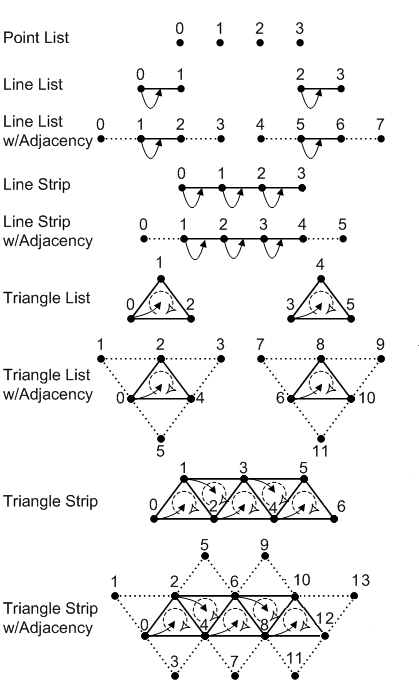
\includegraphics[width=0.45\textwidth]{images/directxprimitives.png}
   \caption{Prymitywy dostępne dla DirectX}
   Źródło: [https://docs.microsoft.com/en-us/windows/win32/direct3d11/images/d3d10-primitive-topologies.png]
   \label{lab:directxprimitive}
\end{figure}

Następnym krokiem jest \emph{Vertex Shader}, który przeprowadza na wierzchołkach takie operacje jak transformacje czy oświetlenie per wierzchołek. Vertex Shader zawsze przyjmuje jeden wierzchołek jako parametr wejściowy i zwraca jeden wierzchołek wyjściowy. Ten krok musi być zawsze obecny, aby potok funkcjonował poprawnie. Jeżeli żadne obliczenia nie są potrzebne na tym etapie należy zdefiniować shader, tak aby ten zwracał wierzchołek, który otrzymał. Jak wyniki z wcześniej przytoczonej tabeli \ref{DirectXShaders} shader może maksymalnie posiadać 16 wektorów wejściowych (32–bitowych), gdzie każdy z nich może zawierać do 4 komponentów (mieć 4 wymiary). Zarówno ten jak i każdy kolejny shader jest pisany w języku HLSL (High Level Shading Language) \cite{directxHLSL}. Listing \ref{lab:directxvertex} zawiera przykład shadera wierzchołków wraz ze strukturą wejściową \emph{VS\_IN}. 

\newpage
\begin{figure}[h!]
  \centering
    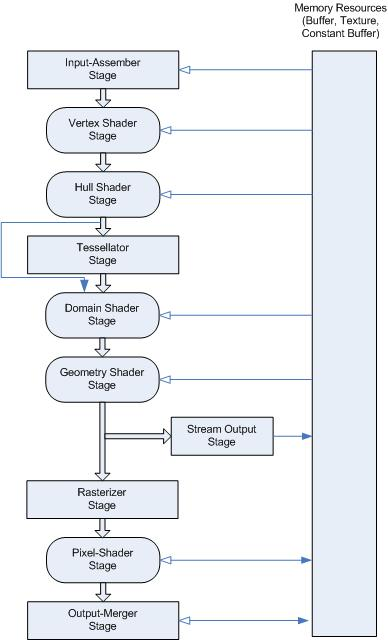
\includegraphics[width=0.55\textwidth]{images/directxpipeline.jpg}
   \caption{Diagram potoku graficznego dla DirectX}
   Źródło: [https://docs.microsoft.com/en-us/windows/win32/direct3d11/images/d3d11-pipeline-stages.jpg]
   \label{lab:directxpipeline}
\end{figure}

\begin{lstlisting}[caption={DirectX, Vertex Shader},captionpos=b,label={lab:directxvertex}]
struct VS_IN{
	float4 pos : POSITION;
	float4 col : COLOR;
	float4 normal : NORMAL;};
PS_IN VS(VS_IN input)
{
	PS_IN output = (PS_IN) 0;
	output.pos = mul(input.pos, worldViewProj);
	output.pos2 = mul(modelMatrix,input.pos);
	output.col = input.col;
	output.normal = mul(modelMatrixInv,input.normal);
	return output;
} 
\end{lstlisting}

\newpage


Następne trzy kroki dotyczą teselacji (proces podziału wielokątów na mniejsze części) realizowanej sprzętowo. Przed pojawieniem się wersji 11 DirectX sterownik wymagał by dostarczyć mu pełną siatkę renderowanego obiektu. Jednak ta metoda była nieefektywna i była wąskim gardłem. Wraz z pojawieniem się modelu shadera nr 5 programista mógł dostarczyć jedynie bazową siatkę o niskiej dokładności, a następnie poinstruować kartę graficzną by ta podzieliła ją na mniejsze części. Ten proces jest implementowany w shaderze powłoki \emph{ang. Hull Shader} i shaderze dziedziny \emph{ang. Domain Shader}. Na rysunku \ref{lab:directxtesselation} przedstawiono wynika działania teselacji sprzętowej z wykorzystaniem DirectX 11 wykonanej na karcie graficznej Radeon HD 5830 \cite{DirectXTesselation}.

\begin{figure}[h!]
  \centering
    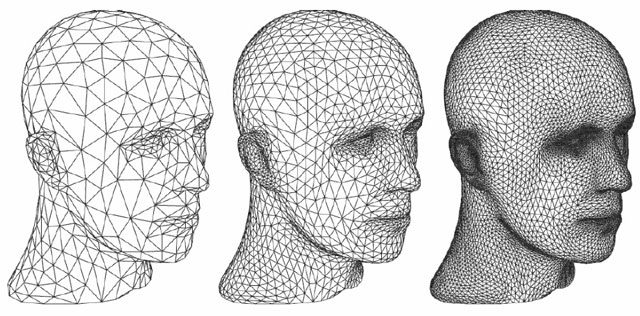
\includegraphics[width=0.45\textwidth]{images/tesselation.jpg}
   \caption{Teselacja sprzętowa z wykorzystaniem DirectX 11}
   Źródło: [http://rastergrid.com/wp-content/uploads/2010/09/fi\_tessellation.png]
   \label{lab:directxtesselation}
\end{figure}

\emph{Geometry shader} tak jak \emph{Vertex Shader} działa na wierzchołkach, z tą różnicą, że ten pierwszy może przyjmować jako dane wejściowe więcej niż jeden wierzchołek. Ten etap pozwala na zwrócenie wielu wierzchołków, które mogą tworzyć nową topologię. W tym kroku możliwa jest implementacja między innymi dynamicznego systemu cząsteczek czy ustawienia osobnego materiału na każdy prymityw. Inną przydatną techniką, która wykorzystuje shader geometrii jest \emph{Billboarding}, czyli rysowanie skomplikowanych obiektów na płaszczyznach skierowanych w kierunku kamery \cite{Billboarding}. \emph{Geometry Shader} realizujący \emph{Billboarding} przedstawiono na Listingu \ref{lab:directxgeometry}. Fraza \emph{maxvertexcount(4)} oznacza, że funkcja może zwracań maksymalnie 4 wierzchołki.

\begin{lstlisting}[caption={DirectX, Geometry Shader},captionpos=b,label={lab:directxgeometry}]
[maxvertexcount(4)]
VS_OUTPUT GS_Billboard(GS_INPUT vert[4])
{
	VS_OUTPUT outputVert;
	for(int i = 0; i < 4; i++)
	{	
		outputVert.Pos = mul(float4(vert[i], 1.0f), WVP);
		outputVert.worldPos = float4(vert[i], 0.0f);
		outputVert.TexCoord = texCoord[i];

		outputVert.normal = float3(0,0,0);
		outputVert.tangent = float3(0,0,0);

		OutputStream.Append(outputVert);
	}
}
\end{lstlisting}
\newpage

Jednym z możliwych etapów następujących po shaderze geometrii jest \emph{Stream–Output Stage}. Jego celem jest ciągłe strumieniowanie danych o wierzchołkach otrzymanych z~poprzednich etapów do bufora (lub buforów) w pamięci. Dane zapisane w taki sposób w~pamięci mogą być ponownie wykorzystane w ponownym cyklu renderowania lub być odczytane przez CPU. Jednym z możliwych zastosowań takiego mechanizmu jest użycie karty graficznej do jednoczesnego wykonania wielu obliczeń niezwiązanych z grafiką, których wykonanie na CPU zajęło by dużo więcej czasu. Aby uruchomić tę część potoku należy wykonać dwa kroki. Najpierw należy w odpowiedni sposób utworzyć shader, z którego będą strumieniowane dane. W tym celu należy wywołać funkcję \emph{CreateGeometryShaderWithStreamOut} na urządzeniu D3D11 (Listing \ref{lab:directxoutputshader}). Drugi krok zakłada utworzenie bufora, w którym będą znajdować się dane wyjściowe (Listing \ref{lab:directxoutputbufer}).\\


\begin{lstlisting}[caption={DirectX, Stream–Output, Utworzenie shadera},captionpos=b,label={lab:directxoutputshader}]
D3D11_SO_DECLARATION_ENTRY pDecl[] =
{
    { "SV_POSITION", 0, 0, 4, 0 }, 
    { "TEXCOORD0", 0, 0, 3, 0 },  
    { "TEXCOORD1", 0, 0, 2, 0 },  
};

D3D11Device->CreateGeometryShaderWithStreamOut( 
pShaderBytecode, ShaderBytecodesize, pDecl, 
    sizeof(pDecl), NULL, 0, 0, NULL, &pStreamOutGS );
\end{lstlisting}


\begin{lstlisting}[caption={DirectX, Stream–Output, Tworzenie bufora},captionpos=b,label={lab:directxoutputbufer}]
ID3D11Buffer *m_pBuffer;
int m_nBufferSize = 1000000;

D3D11_BUFFER_DESC bufferDesc =
{
    m_nBufferSize,
    D3D11_USAGE_DEFAULT,
    D3D11_BIND_STREAM_OUTPUT,
    0,
    0,
    0
};
D3D11Device->CreateBuffer( &bufferDesc, NULL, &m_pBuffer );
\end{lstlisting}

Kolejny etap czyli rasteryzacja (ang. \emph{Rasterizer Stage}) przetwarza informacje o wierzchołkach (kształty lub prymitywy) na obraz złożony z pikseli (Rysunek \ref{lab:raster}). Proces ten ma na celu przekształcenie sceny w obraz, który będzie mógł zostać wyświetlony na ekranie. Rasteryzacja może zostać wyłączona poprzez ustawienie shadera pikseli (\emph{Pixel Shader}) na wartość \emph{null} oraz poprzez ustawienie badania głębokości i szablonów(\emph{depth and stencil testing})na wartość \emph{FALSE}. Kod wyłączający rasteryzacje przedstawiono na Listingu \ref{lab:directxraster}. Ta opcja jest wykorzystywana głównie w sytuacjach, gdy nie chcemy renderować obrazu, a jedynie otrzymać wyniki obliczeń wykonanych we wcześniejszych krokach \cite{DirectXRaster}.
\newpage
\begin{lstlisting}[caption={DirectX, Wyłączanie rasteryzacji},captionpos=b,label={lab:directxraster}]

D3D11_DEPTH_STENCIL_DESC stencil_desc = {
	false,
	D3D11_DEPTH_WRITE_MASK_ALL,
	D3D11_COMPARISON_LESS,
	false,
	D3D11_DEFAULT_STENCIL_READ_MASK,
	D3D11_DEFAULT_STENCIL_WRITE_MASK,
	D3D11_COMPARISON_ALWAYS,
	D3D11_STENCIL_OP_KEEP,
	D3D11_STENCIL_OP_KEEP,
	D3D11_STENCIL_OP_KEEP
}

D3D11Device->PSSetShader(null, null, 0);
D3D11Device->CreateDepthStencilState(stencil_desc);
\end{lstlisting}
\begin{figure}[h!]
  \centering
    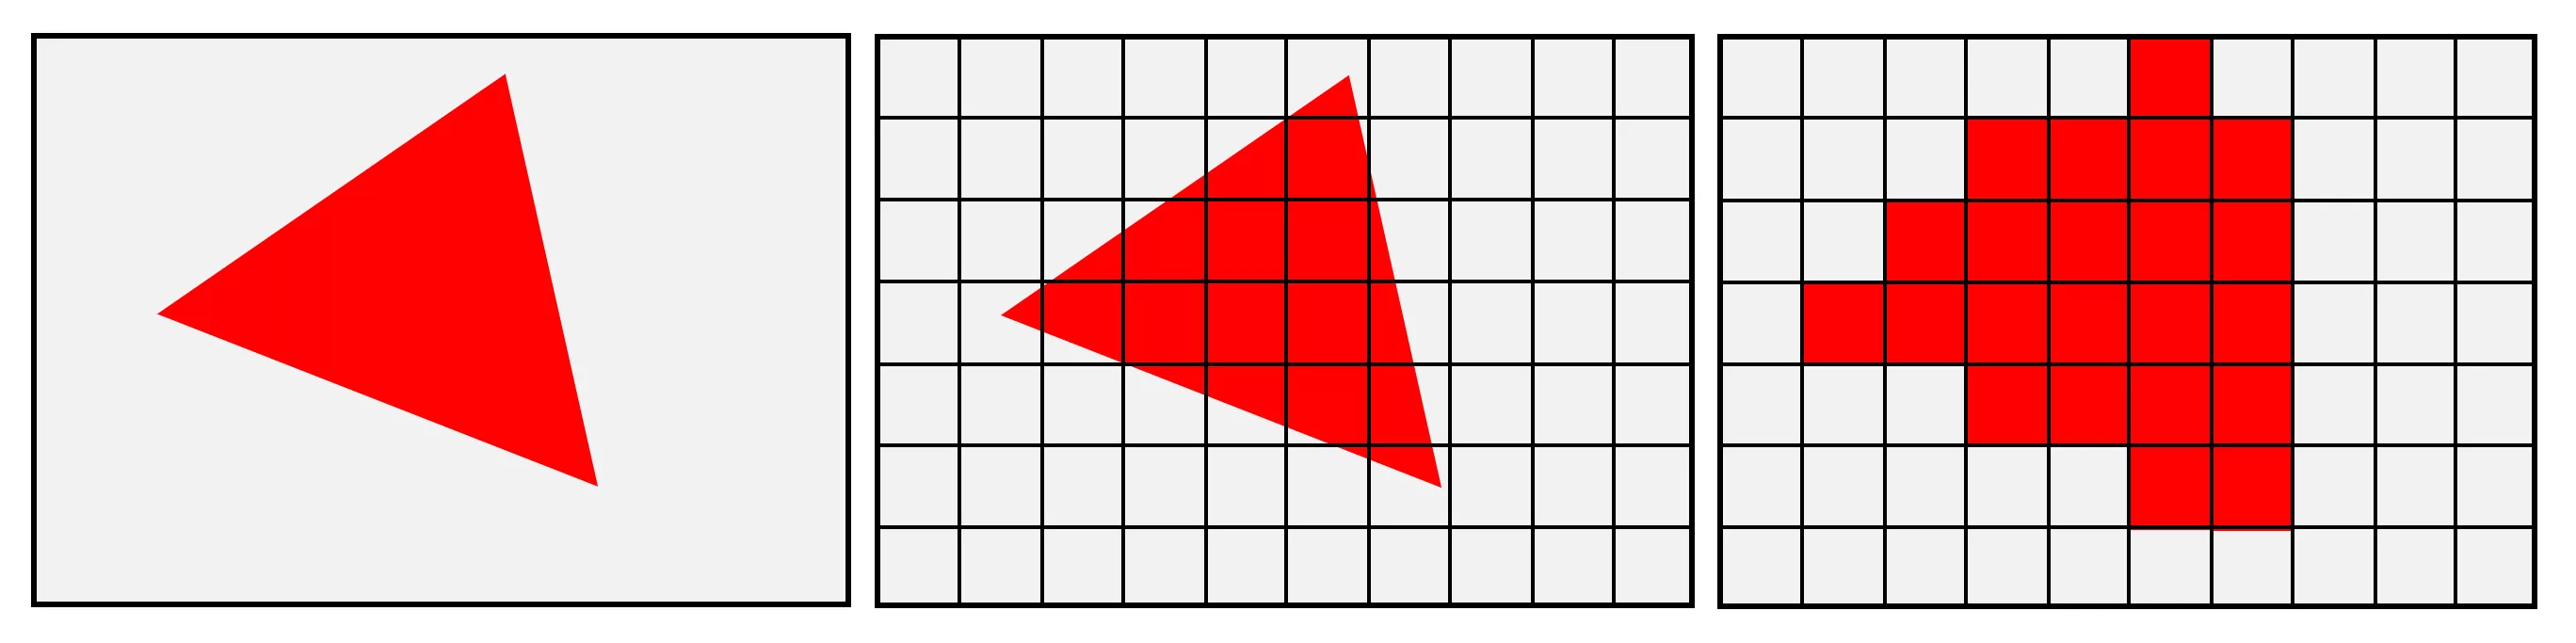
\includegraphics[width=0.50\textwidth]{images/raster.png}
   \caption{Rasteryzacja}
   \label{lab:raster}
\end{figure}

Przedostatnim etapem w procesie renderowania jest programowalny shader pikseli (ang. \emph{Pixel Shader}). Jest on uruchamiany raz na każdy piksel wyprodukowany w procesie rasteryzacji. Pozwala na osiągnięcie złożonych efektów jak oświetlenie czy post–processing. Program shadera łączy otrzymane parametry takie jak stałe, tekstury i inne wartości przypisane do wierzchołków by obliczyć kolor wyjściowych piksela. Ilość możliwych danych wejściowych jest zależna od tego czy shader geometrii został skonfigurowany. Jeżeli shader geometrii jest obecny w potoku, to shader pikseli jest ograniczony do 16 32–bitowych wektorów. W przypadku jego braku liczba to wzrasta do 32. Parametrów wyjściowych może być maksymalnie 8. Przykładową implementację oświetlenia Phonga na shaderze pikseli przedstawiono na Listingu \ref{lab:directxpixelshader}.\\


Ostatni krok \emph{Output–Merger Stage} generuje ostateczny kolor piksela, który znajdzie się na ekranie. Proces ten zawiera wiele elementów, ale najważniejszymi z nich są \emph{Depth–Stencil Testing} oraz \emph{Blending}. Pierwszy z nich na podstawie bufora Z określa który piksel powinien być widoczny, a który jest zasłonięty. To w jaki sposób oba te piksele będą miały wpływ na finalny kolor określa wartość alfa czyli przeźroczystość. Jeżeli piksel bliżej obserwatora jest nieprzeźroczysty, to jego kolor jest kolorem finalnym. Jeśli jednak posiada pewien stopień przeźroczystości, jego kolor jest łączony z kolorem piksela zasłoniętego. To właśnie łączenie określa się mianem \emph{Blending}. Na rysunku \ref{lab:directxdepth} zobrazowano oba te przypadki. Po lewej stronie figura znajdująca się z przodu (czerwony kwadrat) jest częściowo przeźroczysta, więc jej cześć wspólna z zielonych kołem jest połączeniem obu tych kolorów. W prawej części pokazano drugi przypadek, gdy figura jest nieprzeźroczysta. Jak widać część wspólna jest koloru figury bliższej obserwatorowi \cite{DirectXdepth}.

\newpage
\begin{lstlisting}[caption={Pixel Shader, oświetlenie Phonga},captionpos=b,label={lab:directxpixelshader}]

struct PS_IN
{
	float4 pos : SV_POSITION;
	float4 pos2 : POSITION;
	float4 col : COLOR;
	float4 normal : NORMAL;
};

float4 PS(PS_IN input) : SV_Target
{
	float specularStrength = 1;
	float diffuseStrength = 0.7;
	float ambientStrenght = 0.3;
	float4 lightPos = {500.0f, 700.0f, -1000.0f, 1.0f};
	float4 lightDir = normalize(lightPos - input.pos2);
	float4 viewPos = {0.0f, 0.0f, 0.0f, 1.0f};
	float4 viewDir = normalize(viewPos - input.pos2);
	float4 lightColor = {1.0f, 1.0f, 1.0f, 1.0f};
	float4 reflectDir = normalize(
	reflect(-lightDir, input.normal));
	float diff = max(dot(input.normal, lightDir), 0.0f);
	float spec = pow(max(dot(
	viewDir, reflectDir), 0.0), 1024);
	float4 specular = specularStrength * spec * lightColor;
	float4 ambient = ambientStrenght * lightColor;
	float4 diffuse = diffuseStrength * diff * lightColor;


	float4 result = (ambient + diffuse + specular) *
	input.col;
	return result;
}
\end{lstlisting}

\begin{figure}[h!]
  \centering
    
\includegraphics[width=0.70\textwidth]{images/depth.png}
   \caption{Depth Testing oraz Blending}
   \label{lab:directxdepth}
\end{figure}
\newpage
\section{Podobieństwa i różnice}

We wcześniejszych podrozdziałach oba analizowane interfejsy zostały przedstawione, aby przybliżyć sposób ich działania i ich cechy charakterystyczne. Nie ulega wątpliwości, że każdy z nich służy do takiego samego celu, renderowanie grafiki lub ogólniej, do wykonywania obliczeń na karcie graficznej. Istnieją jednak między nimi pewne różnice, które mogą decydować o wyborze jednej technologi nad drugą. W tym rozdziale przedstawione zostaną najistotniejsze różnice i podobieństwa pomiędzy tymi interfejsami.\\

Pierwszą istotną różnicą jest to przez kogo oba te interfejsy są rozwijane. DirectX jest własnością firmy Microsoft oraz jest oprogramowaniem zamkniętym. Kolejne funkcje wydawane są w następujących po sobie wersjach, najczęściej wraz z nowym system operacyjnym. Taki model ma taką zaletę, że istnieje tylko jedna implementacja dostarczona przez firmę Microsoft, przez co kod wykonywany na różnym sprzęcie zachowuje się tak samo. Natomiast wadą jest fakt, że nowe funkcje kart graficznych mogą być w pełni wykorzystane dopiero, gdy firma Microsoft uwzględni je w kolejnej wersji API. W praktyce jednak firmy współpracują ze sobą, tak, aby funkcje dostępne w DirectX były aktualne. Zupełnie inaczej wygląda to w przypadku API OpenGL. Jest to otwarty standard (z wyłączeniem kilku opatentowanych funkcji) nad którym opiekę sprawuje konsorcjum \emph{Khronos Group}. Samo API nie narzuca implementacji, a jedynie definiuje interfejs. Implementacja jest dostarczana przez producenta kart graficznych w formie sterowników. Dzięki temu wraz z pojawieniem się nowej karty graficznej, powstaje nowa wersja sterowania, która jest w stanie w pełni obsłużyć możliwości karty graficznej, dzięki rozszerzeniom. Wadą, która wynika z takiego podejścia jest to, że implementacje różnych producentów mogą się różnić pewnymi szczegółami co może rzutować na że taki sam kod może dawać różniące się w niewielkim stopniu wyniki na różnych kartach graficznych.\\

Kolejną różnicą jest stopień przenośności (ang. \emph{Portability}). Własnościowy DirectX jest implementowany jedynie na systemy operacyjne z rodziny Microsoft Windows oraz na konsolę Xbox. Ponad to, pojawia się wiele problemów z kompatybilnością wsteczną. Istnieją pewne re–implementacje tego API na systemy Unixowe (\emph{Wine} \cite{wine}), ale ze względu na licencje chroniące DirectX oraz trudność w procesie inżynierii odwrotnej takie rozwiązania moją wiele niedoskonałości. OpenGL na tym polu ma dużą przewagę. Jest wieloplatformowy i posiada implementacje na systemy Windows, Linux, Mac OS X, a~nawet dla systemów mobilnych jakich jak Android, iOS, czy BlackBerry. Podsumowanie tych różnic jest widoczne w tabeli \ref{lab:APIdiff}.\\


\begin{table}[h!]

    \centering % instead of \begin{center}
    \caption{Różnice API OpenGL i DirectX}
    		\label{lab:APIdiff}
    \vspace{2mm} % Adjust the height of the space between caption and tabular
\begin{tabular}{|l|l|l|l|}
\hline
\textbf{API} & \textbf{OS} & \textbf{Licenca}& \textbf{Sposób rozwoju} \\ \hline
DirectX & Microsoft Windows, Xbox & Własnościowa & Wersje \\ \hline
OpenGL & Wieloplatformowy & Otwarte oprogramowanie & Rozszerzenia \\ \hline
\end{tabular}
\end{table}

Jak wspomniane we wcześniejszym rozdziale DirectX jest zestawem mniejszych bibliotek. Oprócz renderowanie grafiki może on również zapewniać inną funkcjonalność związaną z obsługą urządzeń wejściowych i multimediów. OpenGL służy jedynie do wykonywania zadań na GPU, w związku z czym w kwestiach po za renderowaniem grafiki programista jest zmuszony korzystać z innych zewnętrznych bibliotek. Jednym z przykładów może być sposób tworzenia okna, do którego będzie renderowany obraz. DirectX z łatwością wykorzysta domyślne okno systemu Windows, natomiast OpenGL do działa potrzebuje biblioteki, która zajmie się tworzeniem i obsługą okna jak np. \emph{GLUT} (Rysunek \ref{lab:opengllib}) \cite{compar}.

\begin{figure}[h!]
  \centering
    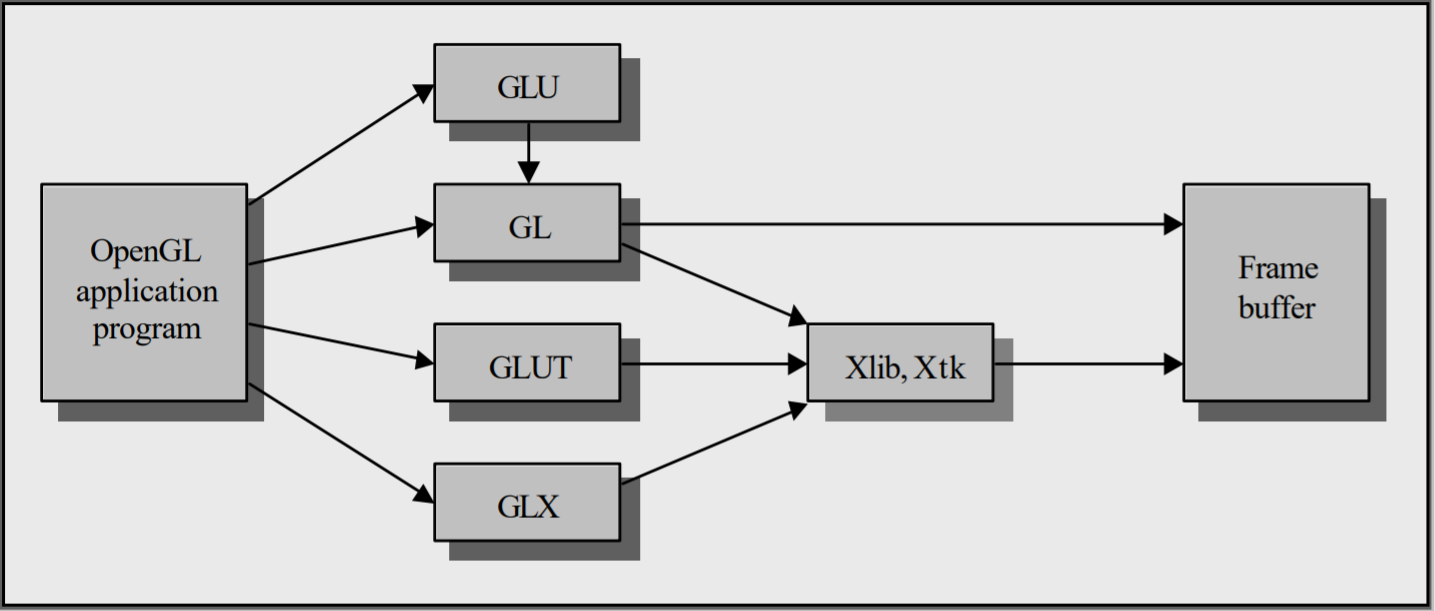
\includegraphics[width=0.70\textwidth]{images/glut.png}
   \caption{OpenGL wraz z biblioteki pomocniczymi}
   Źródło:  \cite{compar}
   \label{lab:opengllib}
\end{figure}

OpenGL jest częściej stosowany w zastosowaniach profesjonalnych takich jak animacje filmowe czy wizualizacje naukowe, natomiast DirectX jest częściej wykorzystywany w~grach komputerowych. Obecnie funkcjonalność obu API jest niemal identyczna i może być stosowana do różnych celów.


\begin{figure}[h!]
  \centering
    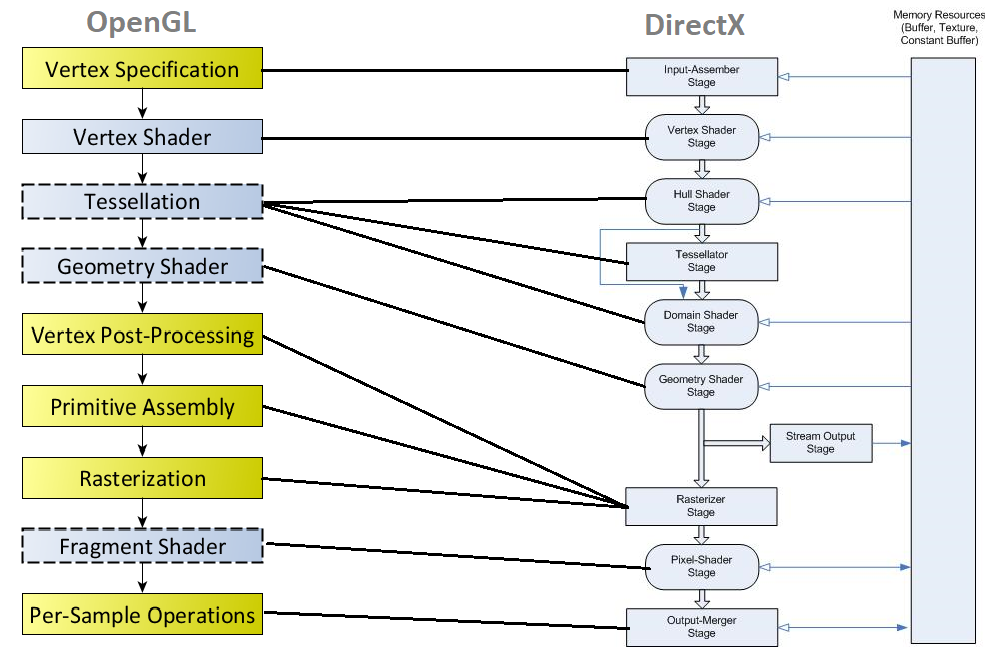
\includegraphics[width=1\textwidth]{images/RenderingPipeline2.png}
   \caption{Potok OpenGL i odpowiadające mu elementu potoku DirectX}
   \label{lab:pipeline2}
\end{figure}
\newpage

Oba interfejsy mogą być stosowane w aplikacjach napisanych w wielu językach. OpenGL jest zbudowany mając w zamyśle maszynę stanów, zaś DirectX jest bardziej zorientowany obiektowo. Wynika to z tego, że DirectX został zaprojektowany jako pewna wizualizacja sprzętu, który jest reprezentowany przez obiekty i sprawia, że programista nie musi komunikować się bezpośrednio z kartą graficzną. Natomiast OpenGL działa jako wspomagany sprzętowo system renderujący. Sprawia to, że pojawiają się pewne funkcjonalne różnice. Jedną z nich jest sposób w jaki zarządzane są zasoby sprzętowe. Direct3D wymaga by za ten aspekt była odpowiedzialna aplikacja, natomiast OpenGL wymaga by zarządzaniem zasobami zajmowała się implementacja. W rezultacie tworzenie aplikacji takich jak silniki graficzne jest mniej skomplikowane, ale tworzenie sterowników jest trudniejsze. Podczas tworzenia oprogramowania z użyciem Direct3D programista musi sam zarządzać zasobami, przez co może je wykorzystać w bardziej optymalny sposób.\\

W kwestii jakości grafiki renderowanej przy użyciu DirectX i OpenGL to są to różnice minimalne. Najczęściej wynikają one z niewielkich różnic w sposobie implementacji modelu oświetlenia. Dobry przykładem takich różnic jest klatka z benchmarku wykonanego za pomocą programu \emph{Unigine Valley} (Rysunek \ref{lab:valley}) \cite{valley};

\begin{figure}[h!]
  \centering
    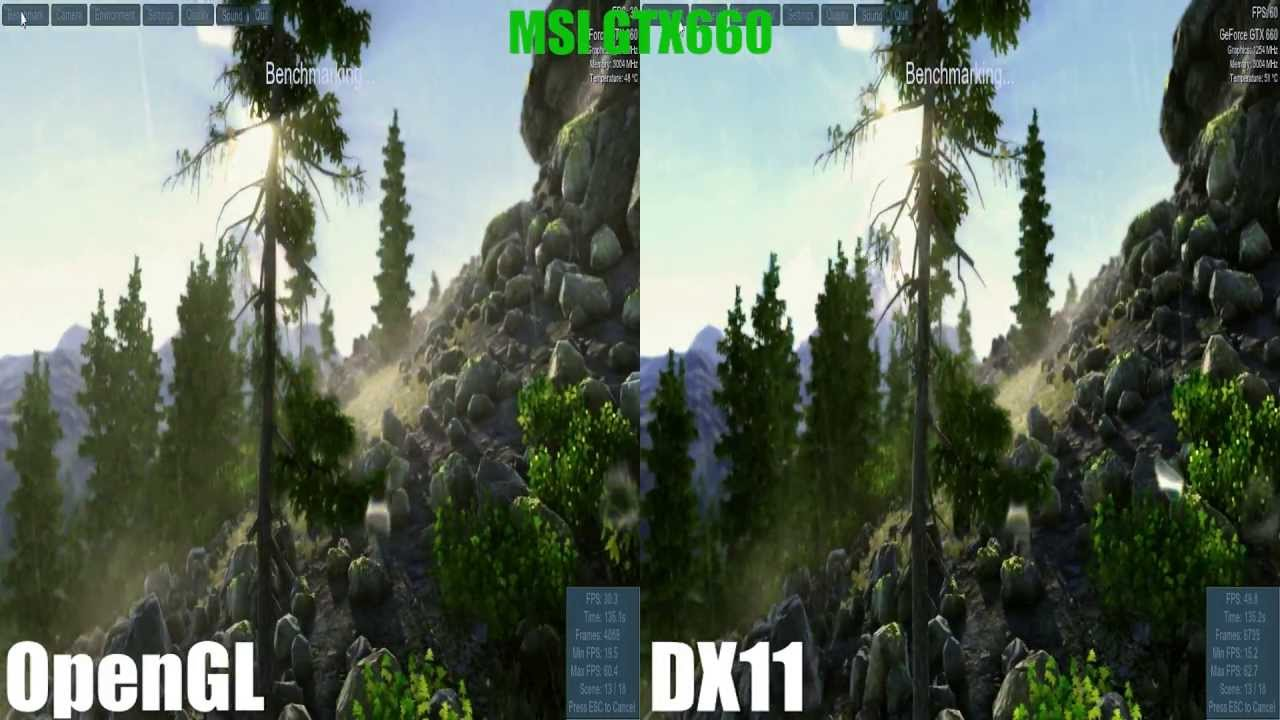
\includegraphics[width=1\textwidth]{images/valley.jpg}
   \caption{Benchmark przy użyciu programu Unigine Valley}
   \label{lab:valley}
\end{figure}

Jak można zauważyć siatki obiektów takich jak drzewa i skały są identyczne. Również wygląd tekstur nałożonych na te obiekty nie ulega zmianie przy wyborze innego API. Jedyna różnica, oświetlenie, prawdopodobnie wynika ze sposobu w jaki są zbudowane shadery w tym konkretnym oprogramowaniu. Wobec tego można stwierdzić, że z punktu widzenia odbiorcy takiego obrazu, wybór API jest bez znaczenia (przy pominięciu kwestii wydajności, która zostanie poruszona w dalszej części pracy).

\newpage
Na rysunku \ref{lab:pipeline2} przedstawiono schematy potoku graficznego dla obu API. Liniami połączone zostały elementy, które pełnią podobną lub taką samą funkcję.W obu przypadkach w pierwszej kolejności występuje krok w którym należy zdefiniować wierzchołki wejściowe. Chodź występuje pewne różnice implementacyjne, proces ten wykonywany jest niemal identycznie. Polega on na dostarczeniu danych o wierzchołkach w formie tablicy jednowymiarowej (jednego miejsca w pamięci), informacji o liczbie wierzchołków oraz ułożeniu danych. Drugi etap to w obu przypadkach shader wierzchołków. W jednym jak i~drugim API pełni on taką samą rolę, wykonuje obliczenia per wierzchołek. Różnice w~tych shaderach wynikają z różnic pomiędzy językami GLSL i HLSL. Na wcześniej przytoczonych Listingach \ref{lab:vertexshader} i \ref{lab:directxvertex} widać wyraźną różnicę pomiędzy dwoma językami. Na uwagę zasługuje sposób w jaki deklaruje się dane wejściowe i wyjściowe. GLSL wymaga by po za funkcję \emph{main} zadeklarować zmienne według formatu zawierającego rodzaj (in – input, out – output, uniform – stała), typ(np. vec4 – wektor 4–wymiarowy,  mat4 – macierz 4x4) oraz nazwę. W HLSL definiuje się strukturę, a wewnątrz niej zmienne według formatu typ (np. float4 – wektor 4–wymiarowy) oraz nazwę. To czy dana struktura jest wejściowa czy wyjściowa jest określane w definicji funkcji realizującej shader. Jeżeli struktura jest zwracana to jest wyjściowa, jeżeli znajduje się w parametrze funkcji jest wejściowa. Przykładowe różnice w sposobie definicji typów zmiennych w obu języka przedstawiono w Tabeli \ref{lab:datatypes}.



\begin{table}[!h]

    \centering 
    \caption{Różnice w definicji typów danych w języka GLSL i HLSL}
    		\label{lab:datatypes}
    \vspace{2mm} 
\begin{tabular}{|p{3cm}|p{3cm}|p{9cm}|}
\hline


\textbf{OpenGL}&\textbf{DirectX}&\textbf{Opis}\\ \hline
uint & unit,dword& liczba całkowita nieujemna\\ \hline
       & min16float& liczba zmiennoprzecinkowa o co najmniej 16–bitowej precyzji\\ \hline
bvecn & booln& wektor typu logicznego o długości n\\ \hline
ivecn & intn&wektor liczb całkowitych o długości n\\ \hline
vecn & floatn&wektor liczb zmiennoprzecinkowych pojedynczej precyzji o długości n\\ \hline
dvecn & doublen&wektor liczb zmiennoprzecinkowych podwójnej precyzji o długości n\\ \hline
matnxm & floatnxm& macierz wielkości n na m liczb zmiennoprzecinkowych pojedynczej precyzji\\ \hline
matn & floatnxn& macierz wielkości n na n liczb zmiennoprzecinkowych pojedynczej precyzji\\ \hline
dmatn & doublematnxn& macierz wielkości n na n liczb zmiennoprzecinkowych podwójnej precyzji\\ \hline
scalar\_type[] & & tablica skalarów wybranego typu\\ \hline
uniform <type> & Buffer<type>& bufor danych, niezmienny w kolejnych iteracjach shadera\\ \hline

\end{tabular}
\end{table}

\newpage

W dalszej części schematu potoku przedstawionego na rysunku \ref{lab:pipeline2} zauważyć można, że proces teselacji w OpenGL odpowiada trzem krokom w DirectX. Dla obu API jest to proces programowalny, lecz DirectX posiada jeden dodatkowy shader. Sprawia to, że programista musi włożyć więcej czasu, aby uzyskać taki sam efekt. Zyskuje natomiast większą kontrolę nad całym procesem. Geometry shader w obu interfejsach pełni taką samą rolę – wykonuje obliczenia per kształt pierwotny. Kolejny krok czyli rasteryzacja został na schemacie OpenGL rozbity na 3 elementy, lecz jest to proces nieprogramowalny i z punktu widzenia dewelopera jest to jeden etap. Oba interfejsy posiadają shader wykonujący obliczenia na każdy piksel otrzymany z wcześniejszego kroku (\emph{Fragment Shader} oraz \emph{PixelShader}). Ich funkcjonalność jest taka sama i tak samo jest w przypadku shadera geometrii różnice wynikają ze stosowanych języków cieniowania. Ostatnie etapy także pełnią taką samą rolę, czyli przygotowują otrzymane piksele do wyświetlenia na ekranie. Różnice w sposobie działania potoku są minimalne i mają znikomy wpływ na produkt końcowy.  W tabeli \ref{lab1:comparetable123} zaczerpniętej z książki \emph{OpenGL Game Programming} \cite{book} znajduje się podsumowanie pewnych cech i funkcji charakterystycznych dla obu interfejsów.

\begin{table}[!h]

    \centering 
    \caption{Porównanie cech i mechanizmów API}
    		\label{lab1:comparetable123}
    \vspace{2mm} 
\begin{tabular}{|l|l|l|}
\hline

\textbf{Feature} &	\textbf{OpenGL}	&\textbf{DirectX}\\ \hline
Vertex Blending&	N/A	Yes&	\\ \hline
Multiple Operating Systems&	Yes&	No\\ \hline
Development&	Multiple member Board	&Microsoft\\ \hline
Thorough Specification&	Yes	&No\\ \hline
Two–sided lighting	&Yes&	No\\ \hline
Volume Textures&	Yes&	No\\ \hline
Hardware independent Z–buffers&	Yes	&No\\ \hline
Accumulation buffers&	Yes&	No\\ \hline
Stereo Rendering&	Yes&	No\\ \hline
Point–size/line–width attributes&	Yes	&No\\ \hline
Picking&	Yes&	No\\ \hline
Parametric curves and surfaces&	Yes&	No\\ \hline
Cache geometry&	Display Lists&	Vertex Buffers\\ \hline
System emulation&	Hardware not present&	Let app determine\\ \hline
Interface&	Procedure calls&	COM\\ \hline
Source Code&	Sample&	SDK Implementation\\ \hline

\end{tabular}
\end{table}


Każde oprogramowanie cechuje się pewnym poziomem wydajności, który często decyduje o jego użyteczności. Nie inaczej jest w przypadku implementacji interfejsów graficznych. Najważniejszymi parametrami, które określają wydajność API graficznego jest czas w jakim są w stanie wykonać pewne zadanie (najczęściej jest to renderowanie obrazu) oraz ilość pamięci potrzebnej do jego  ukończenia. Jako, że implementacje API są skomplikowanym i złożonym oprogramowaniem możliwość analitycznej oceny ich wydajności jest ograniczona. Z związku z tym najlepszym rozwiązaniem jest wykonanie pomiarów czasu wykonania zadania i zajętości pamięci przez program. Podjęto wiele takich prób, używając różnych metod, co pozwoliło na poszerzenie wiedzy w tej dziedzinie. Mimo to, jest to wciąż otwarty temat i aby móc dokonać porównania wydajności API DirectX 11 i~OpenGL 4 wymaga dogłębnej analizy.

\chapter{Przegląd literatury}

W tym rozdziale zostaną przedstawione najważniejsze publikacje omawiające tematykę wydajności w dziedzinie interfejsów graficznych i programów cieniujących. Ocena i~porównanie wydajności tych API musi odbywać się w oparciu o wykonane pomiary. Rozdział ten ma na celu przybliżenie oraz analizę pracy wykonanej na tym polu, stosowanych metod pomiarów, wykorzystanych technologii oraz otrzymanych wyników. Pozwoli to na zebranie dotychczasowej wiedzy, a następnie wykorzystanie jej jako punktu wyjścia do dalszych badań i uzupełnienia potencjalnych luk.


Podczas poszukiwania prac dotyczących zagadnień związanych z API graficznymi natrafiono na dokumenty, które opisują konkretne elementy danego interfejsu lub porównywały jego mechanizmy do innego API. Jedną z takich prac jest \emph{Comparison of Technologies for General-Purpose Computing on Graphics Processing Units} \cite{lit1}. Analizuje on technologie \emph{CUDA}, \emph{OpenCL}, \emph{DirectCompute} oraz \emph{OpenGL} pod kątem zastosowania ich w obliczeniach ogólnego użytku realizowanych na procesorze graficznym (\emph{ang. general-purpose computation on graphics processing units, GPGPU}). Autor wykonał pomiary czasu wykonywania się algorytmów takich jak dyskretna i szybka transformata Fouriera, kompresja obrazu, przekształcenia liniowe czy sortowanie.  Wyniki, które otrzymał autor wskazują, że różnice w wydajności wybranych API są minimalne i zależne od sprzętu na którym wykonywanie są badania. Praca ta jest wartościowa i wskazuje kierunek dalszych badań. Należy jednak zaznaczyć czego owa praca nie dotyczy oraz jakie elementy nie zostały uwzględnione. Nie poruszono kwestii API DirectX, które zdominowało rynek gier komputerowych i obok OpenGL jest najczęściej wykorzystywanym API graficznym. Drugim elementem, który pozostaje kwestią otwartą jest porównanie czasy wykonania się całego potoku graficznego czyli renderowania sceny. Praca opisuje operacje na API dla GPGPU, więc pomija dalsze etapy potoku oraz tematy związane z pamięcią VRAM (Video RAM). Na Rysunkach \ref{lab:liter11}, \ref{lab:liter12} pokazano wyniki, które w swojej pracy przedstawił autor. są to wykresy, które zawierają informacje o tym ile czasu potrzebowała karta graficzna na wykonanie jednowymiarowej i  dwuwymiarowej transformaty Fouriera przy różnej wielkości przetwarzanych danych. Jak można zauważyć wykonano badania dla wielu interfejsów, lecz brak DirectX. Wyniki te pokazują, że istnieje różnica w czasie wykonania zadania przez różne API, lecz jest zależna od użytej karty graficznej.\\
\newpage
\begin{figure}[h!]
  \centering
    \includegraphics[width=0.38\textwidth]{images/lit/1.png}
   \caption{Średni czas wykonania jednowymiarowej transformaty Fouriera}
   Źródło: \cite{lit1}
   \label{lab:liter11}
\end{figure}
\begin{figure}[h!]
  \centering
    \includegraphics[width=0.38\textwidth]{images/lit/1.png}
   \caption{Średni czas wykonania dwuwymiarowej transformaty Fouriera}
   Źródło: \cite{lit1}
   \label{lab:liter12}
\end{figure}
\newpage

Kolejna praca \emph{A Comparison of Real Time Graphical Shading Languages} \cite{lit2} dotyczy porównania języków cieniowania HLSL oraz GLSL. Dobrze opisano i porównano cechy tych językach z różnych punktów widzenia. Jednym z nim jest przybliżenie tzw. \emph{Maintenence Features}, czyli sposobów w jaki może być organizowany kod, tak aby był czytelniejszy i łatwiejszy w rozwoju. Dalej autor omawia różnice w sposobie przekazywania parametrów do potok graficznego oraz architekturę obu API. Najciekawszym fragmentem pracy jest rozdział dotyczący porównania wydajności. Dla każdego z analizowanych języków wykonano badania shaderów wierzchołków i pikseli. Polegały one na pomiarze czasu renderowania sceny przy pewnej założonej intensywności obliczeń w programach cieniujących. Dla shadera wierzchołków wykonano przekształcenie 50 000 wierzchołków pewną funkcją trygonometryczną. Dla shadera pikseli intensywności obliczeniowa została zapewniona poprzez implementację oświetlenia Phonga. Praca ta stanowiła inspirację dla części z wykonanych badań, szczególnie dla fragmentu dotyczącego badań wpływu intensywności obliczeń w shaderach na całkowity czas renderowania sceny. Niestety w~przytoczonej pracy wykonano zbyt mało pomiarów i wyniki są niejednoznaczne. W Tabeli \ref{lab:tabLib1} przytoczono jedyne wyniki liczbowe, które w swojej pracy podaje autor. Ciężko jest na ich podstawie wysunąć wnioski. Ponad to jest to praca opublikowana w 2005 roku i zawiera wiele przestarzałych informacji. W tej dziedzinie postęp jest tak szybki, że w~ciągu dekady duża część wiedzy przestaje być aktualna i wymaga aktualizacji.


\begin{table}[h!]

    \centering % instead of \begin{center}
    \caption{Wyniki testu w formie klatek na sekundę}
    		\label{lab:tabLib1}
    \vspace{2mm} % Adjust the height of the space between caption and tabular
\begin{tabular}{|l|l|l|l|}
\hline
\textbf{Test/Language} & \textbf{HLSL} & \textbf{Cg 1.3 (OpenGL)}& \textbf{GLSL} \\ \hline
Vertex bound & 123 & 120 & 115 \\ \hline
Fragment bound & 102 & 91 & 94 \\ \hline
\end{tabular}
\end{table}



Następna pozycja z literatury, czyli \emph{An Exploratory Study Of High Performance Graphics Application Programming Interfaces} \cite{lit3} bada różnice w wydajności pomiędzy API niskopoziomowymi (DirectX 12, Vulcan), a tymi z~wyższego poziomu abstrakcji (DirectX 11, OpenGL). Autor podejmuje się analizy tych interfejsów w celu walidacji ich zalet i~wad w stosunku do starszych odpowiedników. Oprócz szczegółowego opisu omawianych API wykonano również pomiary wydajności. Polegały on na pomiarze klatek na sekundę (ang. frames per second, FPS) osiąganych w pewnych grach komputerowych takich jak np. \emph{Ashes Of Singularity}  co pokazano na przytoczonych Rysunkach \ref{lab:liter21} i \ref{lab:liter22} i Tabeli \ref{lab:tabLib2}. Wnioski, które otrzymuje autor wskazują, że niskopoziomowe API dostarczają wzrostu wydajności, lecz prawidłowa implementacja funkcjonalności jest trudniejsza. \\

\begin{table}[h!]

    \centering % instead of \begin{center}
    \caption{Czas renderowania klatki}
    		\label{lab:tabLib2}
    \vspace{2mm} % Adjust the height of the space between caption and tabular
\begin{tabular}{|l|l|l|}
\hline
\textbf{Object Count} & \textbf{ms/frame Vulcan} & \textbf{ms/frame OpenGL}\\ \hline
256 & 0.57 & 0.84 \\ \hline
1k & 0.95 & 2.50 \\ \hline
4k & 3.18 & 8.33 \\ \hline
16k & 12.94 & 30.86 \\ \hline
64k & 47.44 & 123.62 \\ \hline
\end{tabular}
\end{table}

\newpage

\begin{figure}[h!]
  \centering
    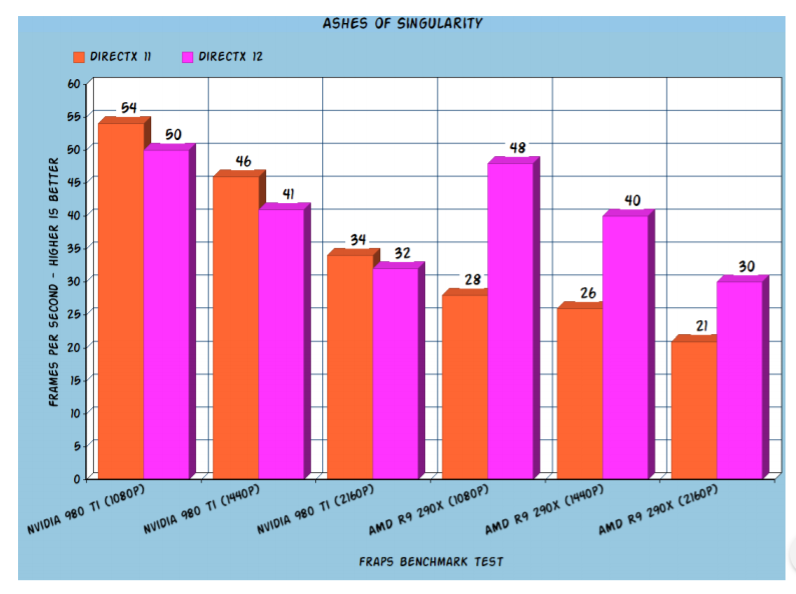
\includegraphics[width=0.85\textwidth]{images/lit/11.png}
   \caption{Liczba klatek na sekundę w grze Ashes Of Singularity}
   Źródło: \cite{lit3}
   \label{lab:liter21}
\end{figure}

\begin{figure}[h!]
  \centering
    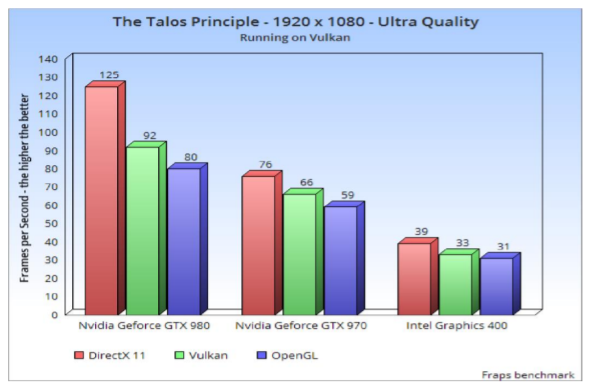
\includegraphics[width=0.85\textwidth]{images/lit/12.png}
   \caption{Liczba klatek na sekundę w grze The Talos Principle}
   Źródło: \cite{lit3}
   \label{lab:liter22}
\end{figure}

\newpage

Kolejna praca również dotyka tematyki języków cieniowania. \emph{Porównanie Wydajności Języków Cieniowania Cg I Hlsl} \cite{lit4} zawiera opis 10 testów szybkości wykonania programów cieniujących. Wśród nich można znaleźć:

\begin{itemize}
  \item przekształcenie wierzchołków,
  \item operacje na teksturach (przesunięcie i nałożenie),
  \item nałożenie tekstury kubicznej na obiekt,
  \item symulowanie załamania światła,
  \item test chromatycznego rozszczepienia światła,
  \item technika rzucania cienia przez obiekt na samego siebie.
\end{itemize}

Niestety brak dokładniejszego opisu przeprowadzonych testów, oraz odniesienia do języka GLSL. Praca stwierdza, że język HLSL jest co najmniej tak szybki (a częściej szybszy) jak język CG, a wynik zależy od samego testu (Rysunek \ref{lab:liter3}).


\begin{figure}[h!]
  \centering
    \includegraphics[width=0.8\textwidth]{images/lit/3.png}
   \caption{Porównanie średnich czasów wykonania dla różnych testów}
   Źródło: \cite{lit4}
   \label{lab:liter3}
\end{figure}


Ostatnia pozycja z literatury chodź jest porównaniem to nie zawiera pomiarów. Autor pracy \emph{3D APIs in Interactive
Real-Time Systems:Comparison of OpenGL, Direct3D and Java3D.} \cite{compar} opisuje tytułowe API i stara się przybliżyć czytelnikowi sposób ich działania. Ponadto zawiera przykładowe programy, które są pomoce przy budowie własnego oprogramowania. Podczas pisania pracy dokument ten stanowił źródło wiedzy o potoku graficznym i wewnętrznych procesach zachodzących w API OpenGL i DirectX.
\newpage
Chodź wykonano pewną pracę w dziedzinie analizy wydajności interfejsów graficznych to niektóre kwestie nadal nie zostały poruszone. Porównano wiele różnych API graficznych, ale brakuje dobrze opisanej analizy wydajnościowej dwóch obecnie najpopularniejszych interfesów OpenGL 4 oraz DirectX 11. Ponad to w literaturze brakuje informacji o wydajności działania pojedynczych mechanizmów rzeczonych API takich jak tryb usuwania niewidocznych powierzchni. W pracy podjęto próbą uzupełnienia tej luki.



\chapter{Badania}

W tym rozdziale przedstawiono badania dotyczące zagadnienia wydajności API graficznych. W pierwszej kolejności opisano plan badań, w którym zawarto informacje o~tym czym jest wydajność oraz jak ją zmierzyć. Wyszczególniono jakie parametry zostaną poddane pomiarom, w jakich warunkach i w jakim celu. Kolejny podrozdział przedstawia środowisko badacze wykorzystane do wykonania badań. W głównej mierze skupia się na sposobie w jaki został zbudowany silnik graficzny – główne narzędzie badawcze pracy. Opisano w nim sposób implementacji silnika wraz z użytymi technologiami. Ostatni podrozdział pokazuje wyniki badań wraz analizą i podsumowaniem rezultatów w oparciu o~dane zilustrowane na wykresach. Celem tego rozdziału jest przedstawienie procesu badania wydajności analizowanych API i opisanie otrzymanych wyników.


\section{Plan badań}


Badania zostały podzielone na dwie grupy. Pierwsza z nich dotyczy pomiaru czasu renderowania sceny w określonych warunkach. Badania te mają na celu sprawdzenie wpływu tych czynników na czas generowania klatki. Taka informacja może być pomocna dla dewelopera zarówno podczas wyboru API jako i samej implementacji aplikacji. Posiadając wiedzę, które elementy potoku graficznego mają największy wpływ na wydajność, możliwa jest lepsza optymalizacja oprogramowania. Te warunki to:

\begin{itemize}
  \item intensywne obliczenia w shaderach – przekształcenie MVP (Model View Projection) dla shadera wierzchołków, oświetlenie Phonga dla shadera pikseli/fragmentów,
  \item minimalizacja obliczeń wykonywanych w shaderze pikseli – wyłączenie oświetlenia,
  \item minimalizacja obliczeń  wykonywanych w obu shaderach – wyłączenie oświetlenia oraz przekształcenia MVP,
  \item włączony tryb rysowania linii (ang. wireframe),
  \item włączony tryb usuwanie niewidocznych powierzchni (ang. face culling).
\end{itemize}

Pomiar czasu zostanie wykonany za pomocą klasy \emph{StopWatch}, która jest domyślnie dostępna w języku C\#. Pozwala ona na zmierzenie czasu, który upłynął pomiędzy kolejnymi wywołaniami właściwości \emph{ElapsedMilliseconds} z dokładnością do 1ms. Na listingu \ref{lab:stopwatch} przedstawiono przykład pomiaru czasu z jej pomocą (symbolem "(...)" oznaczono czynności, które podlegają pomiarowi).


\begin{lstlisting}[caption={Klasa StopWatch – przykładowe użycie},captionpos=b,label={lab:stopwatch}]

startTime = _stopwatch.ElapsedMilliseconds;
(...)
elapsedTime = _stopwatch.ElapsedMilliseconds - startTime;
\end{lstlisting}

Dla API OpenGL mierzony jest czas wykonania funkcji \emph{gl.DrawArrays(...)}, a dla DirectX \emph{\_context.Draw(...)}. Są to funkcje, które rozpoczynają proces renderowania i wstrzymują wykonywanie się kodu na CPU do momentu ukończenia obliczania klatki.

Druga grupa jest związana z innymi ważnymi parametrami wydajnościowymi:


\begin{itemize}
  \item czas przesyłania danych do pamięci VRAM,
  \item czas kompilowania shaderów,
  \item stopień wykorzystania GPU,
  \item ilość zajmowanej pamięci VRAM.
\end{itemize}


Czas przesyłania danych oraz kompilowania shadera został zmierzony tą samą metodą jak czas renderowania sceny. Dla DirectX wysyłanie danych odbywa się poprzez wywołanie funkcji \emph{D3D11.Buffer.Create(...)}, a dla OpenGL \emph{gl.BufferData(...)}. W API OpenGL shader jest kompilowany przy użyciu metody \emph{shaderProgram.Create(...)}, a~w~DirectX \emph{D3D11.PixelShader(...)} i \emph{D3D11.VertexShader(...)}. Badania dla dwóch ostatnich pozycji zostaną wykonane przy użyciu programu zewnętrznego \emph{TechPowerUp GPU-Z}. Stopień wykorzystania GPU oznacza ile procent z dostępnej częstotliwości zegara jest aktualnie wykorzystywane i jest obliczane za pomocą wzoru:
\begin{equation} 
\label{metric}
L = \frac{freq}{freqMax}100\%
\end{equation}
\begin{itemize}
  \item L – obciążenie [\%],
  \item freq – zmierzona częstotliwość zegara GPU,
  \item freqMax – maksymalna dostępna częstotliwość zegara GPU.
\end{itemize}

Ostatnim badanym parametrem jest ilość zajętej pamięci VRAM przy określonej liczbie wierzchołków. Jako, że karty posiadają ograniczoną ilość pamięci GDDR, nadmiar danych znajduje się w specjalnie wydzielonej części pamięci RAM DDR tworząc tzw. pamięć wirtualną. Aby móc porównać wydajność miedzy różnymi kartami, które posiadają różną ilość pamięci GDDR, zmierzona zostanie suma tych pamięci.\\

Wstępne badania wykazały, że podczas procesu renderowania występuje wiele elementów, które pochłaniają stałą ilość czasu i sumują się maksymalnie do 1 ms. W związku z tym, aby zminimalizować ich wpływ na pomiary, badania zostały wykonane dla takiej liczby wierzchołków, która pozwali na osiągnięcie czasu renderowania powyżej 10 ms (minimum 2 miliony wierzchołków). Ponad to, dla każdego wykonanego testu pominięto pierwsze 10 pomiarów, które często były zakłócone przez proces inicjalizacji API.\\

Dla wszystkich pomiarów zostaną wykonane badania na trzech stacjach roboczych. Każda z nich jest zaopatrzona w kartę graficzną innego producenta. Ma to na celu sprawdzenie jak implementacje API graficznych różnych producentów sprawdzają się w konkretnych zadaniach. Dzięki temu możliwe będzie określenie, czy ewentualne różnice w wydajności wynikają z konkretnej implementacji API, czy z samej jego architektury. W tabelach \ref{lab:comps1}, \ref{lab:comps2}, \ref{lab:comps3} przedstawiono specyfikację stacji roboczych użytych do wykonania badań.\\

Należy mieć na uwadze to, że podczas wykonywania pomiarów na stacjach roboczych działają również inne aplikacje, które również mogą korzystać z zasobów komputera. Efekt ten został zminimalizowany poprzez wyłączenie wszystkich zbędnych procesów, ale jego całkowite wyeliminowanie jest niemożliwe. Aby mieć pewność, że otrzymany wynik nie jest anomalią każdy pomiar zostanie wykonany stukrotnie. Po przeprowadzeniu badań wstępnych ustalono, że współczynnik zmienności dla wykonanych pomiarów jest stosunkowo niski (0.1 – 0.2), więc dane zostaną uśrednione za pomocą średniej arytmetycznej.

\begin{table}[!h]

    \centering 
    \caption{Specyfikacja komputera nr 1}
    		\label{lab:comps1}
    \vspace{2mm} 
\begin{tabular}{|l|l|}
\hline

\textbf{Komponent}&	\textbf{Model}\\ \hline
Karta graficzna & Intel UHD Graphics 620  \\ \hline
Procesor & Intel Core i7-8650U  \\ \hline
Pamięć RAM & 16 GB, DDR 4, 3200 MHz \\ \hline
Płyta główna & Dell Inc. 0MM81M \\ \hline
System operacyjny & Windows 10 \\ \hline
\end{tabular}
\end{table}

\begin{table}[!h]

    \centering 
    \caption{Specyfikacja komputera nr 2}
    		\label{lab:comps2}
    \vspace{2mm} 
\begin{tabular}{|l|l|}
\hline

\textbf{Komponent}&	\textbf{Model}\\ \hline
Karta graficzna & Nvidia GeForce GTX770  \\ \hline
Procesor & Intel Core i5-4570   \\ \hline
Pamięć RAM  & 8GB, DDR3, 1600MHz \\ \hline
Płyta główna & ASRock B85 \\ \hline
System operacyjny & Windows 10  \\ \hline
\end{tabular}
\end{table}

\begin{table}[!h]

    \centering 
    \caption{Specyfikacja komputera nr 3}
    		\label{lab:comps3}
    \vspace{2mm} 
\begin{tabular}{|l|l|}
\hline

\textbf{Komponent}&	\textbf{Model}\\ \hline
Karta graficzna& AMD Radeon HD 5700  \\ \hline
Procesor & AMD Phenom II X6 1050T  \\ \hline
Pamięć RAM & 8GB DDR3 2333 MHz \\ \hline
Płyta główna &  ASUSTek Computer Inc. M4A77T\\ \hline
System operacyjny & Windows 7  \\ \hline
\end{tabular}
\end{table}

\newpage
\section{Środowisko badawcze}
Aby przeprowadzić dokładne i rzetelne badania w pierwszej kolejności należy zbudować odpowiednie narzędzia badawcze. W tym rozdziale przedstawiony został proces budowy takiego narzędzia – silnika graficznego. Opisano założenia jakimi się kierowano, wykorzystane technologie oraz sam sposób implementacji.
\subsection{Założenia i wymagania}
Silnik graficzny, który zostanie użyty do badania wydajności musi spełniać pewne kryteria. Pierwszym wymogiem jest, aby działał w dwóch trybach – OpenGL oraz DirectX. Jest to szczególnie wymagające wymaganie, ponieważ w praktyce wymaga dwukrotnej implementacji tej samej logiki dla obu interfejsów. Dlatego ważne jest, aby tak zaprojektować silnik, aby minimalizować powielającą się logikę. Operacje takie tak tworzenie obiektu 3D, generowanie wektorów normalnych czy przygotowanie danych wejściowych do shaderów powinno odbywać się tylko jednym miejscu.
\\

Drugim elementem, którego obecność w silniku jest niezbędna jest możliwość generowania obiektów 3D złożonych z dużej ilości wierzchołków (rzędu milionów). Sam kształt tych obiektów jest bez znaczenia tak długo, dopóki wszystkie wierzchołki znajdują się na scenie, a badania wykonano dla takiej samej figury. W pracy zdecydowano się na wybór sześcianu ze względu na prostotę tej figury. Duża ilość wierzchołków zostanie osiągnięta poprzez rekurencyjny podział trójkątów z których został zbudowany na mniejsze trójkąty. Na rysunku \ref{lab:points} przedstawiono model sześcianu zbudowany z 589824 wierzchołków. \\



Następnym wymaganiem jest zawarcie w silniku wszystkich elementów, które mają zostać poddane badaniom. Spośród nich można wyszczególnić oświetlenie Phonga implementowane w shaderze fragmentów/pikseli. Powinno ono prawidłowo modelować każdą z~trzech składowych światła(\emph{ambient}, \emph{diffuse}, \emph{specular}) jednocześnie minimalizują ilość wykonywanych zbędnych obliczeń. Algorytm Phonga musi być zaimplementowany osobno dla języka GLSL oraz HLSL.
Innymi pomniejszymi elementami, które muszą być zawarte w silniku jest są takie elementy jak \emph{face culling} czy tryb \emph{wireframe}. Są one częścią API, lecz do ich prawidłowego działania wymagana jest odpowiednia konfiguracja potoku.\\

Elementem, który nie jest bezpośrednio powiązany z renderowaniem sceny, ale jego obecność jest istotna jest możliwość poruszania kamerą po scenie przy pomocy klawiatury i myszy. Funkcjonalność ta nie bierze udziału w badaniach, lecz była pomocna przy usuwaniu błędów oraz wizualizacji wygenerowanego obiektu.
Ostatnim wymaganiem jest możliwość wykonywania pomiarów czasu wykonywania się poszczególnych elementów. Pomiary będą wykonywane wielokrotnie a wyniki będą zapisywane do plików. Ponad to musi być to pomiar zapewniający odpowiednią dokładność (milisekundy). Całość musi być stworzona tak, aby mieć możliwość wykonywania badań na różnych stacjach roboczych, bez ingerencji w kod programu. Podsumowując, silnik powinien mieć następujące cechy:
\newpage
\begin{itemize}
  \item obsługa OpenGL 4 oraz DirectX 11,
  \item generowanie obiektów o ilości wierzchołków liczonych w milionach,
  \item możliwość włączenia opcji \emph{Wireframe},
  \item możliwość włączenia opcji ukrywania niewidocznych powierzchni (ang. \emph{FaceCulling}),
  \item poruszanie kamerą przy pomocy myszy i klawiatury,
  \item wykonywanie pomiaru czasu i zapis wyników do pliku.
\end{itemize}

\begin{figure}[h!]
  \centering
    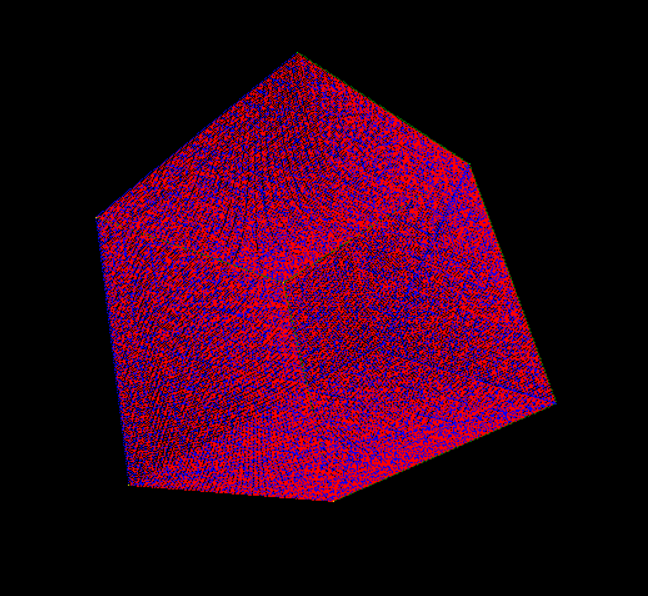
\includegraphics[width=0.8\textwidth]{images/points.png}
   \caption{Sześcian zbudowany z 589824 wierzchołków (wizualizacja wierzchołków)}
   \label{lab:points}
\end{figure}
\newpage
 

\subsection{Technologie}

Klasycznie większość aplikacji graficznych jest tworzona z użyciem języka C++. Jednak aby zapewnić szybki proces rozwoju silnika graficzne, jak i wyeliminować potrzebę manualnego zarządzania pamięcią oprogramowanie zostało oparte o język C\#. Jest to zorientowany obiektowo język programowania ogólnego zastosowania, który do uruchomienia wymaga środowiska \emph{.NET Framework} , \emph{.NET Core}, \emph{Mono} lub \emph{DotGNU}. Zdecydowano się na platformę \emph{.NET Core}, ponieważ jest to standard najnowszy, wspierający wiele użytecznych funkcji i bibliotek. Język C\# posiada wygodną funkcję automatycznego odśmiecania pamięci (\emph{ang. garbage collection}), dzięki czemu programista jest zwolniony z tego obowiązku oraz wyeliminowano problem wycieków pamięci. Na listingu  \ref{lab:csharp} przedstawiono przykładowy kod w języku C\#.

\begin{lstlisting}[caption={Przykładowy kod w języku C\#},captionpos=b,label={lab:csharp}]

using System;

public class PrzykladowaKlasa
{
    public static void Main()
    {
        Console.WriteLine("Podaj swoje imie:");
        string imie = Console.ReadLine();
        Console.WriteLine("Twoje imie to: " + imie);
        Console.WriteLine("Wcisnij dowolny klawisz by zakonczyc.");
        Console.ReadKey();
    }
}
\end{lstlisting}

Aby móc rozpocząć implementację silnika graficznego należy posiadać uchwyty (\emph{ang. handles}) do funkcji z API. Najprostszym rozwiązaniem jest użycie bibliotek, które wyręczaj programistę. Do obsługi API DirectX wybrano bibliotekę \emph{SharpDX} \cite{sharpdx}. Jest on niskopoziomowym "opakowaniem" \emph{wrapper} API DirectX, który większość swoich usług udostępnia za pomocą interfejsu COM (\emph{Component Object Model}). Bazowym interfejsem obiektów COM jest \emph{IUnknown} i posiada metody:

\begin{itemize}
  \item int AddReference(),
  \item int ReleaseReference(),
  \item HRESULT QueryInterface(ref Guid interfaceGuid, out IntPtr pComObj).

\end{itemize}

Obiekt COM posiada wewnętrzny licznik referencji i jest zwalniany, gdy licznik spadnie do 0 i wywołana zostanie metoda \emph{ReleaseReference()}. Wszystkie obiekty biblioteki \emph{SharpDX} dziedziczą po obiekcie \emph{ComObject} i implementują interfejs \emph{IDesposable}. Dzięki temu zasoby mogą być w prosty sposób zwalnianie poprzez wywołanie metody \emph{Dispose()}.
\newpage
SharpDX posiada system obsługi błędów. Prawie wszystkie API systemu Windows (w tym DirectX) zwracają rezultat w postaci liczby całkowitej nazwanej \emph{HRESULT}. W zależności od wartości można określić, czy metoda została wykonana poprawnie.

\begin{itemize}
  \item HRESULT < 0 – błąd,
  \item HRESULT == 0 – sukces),
  \item HRESULT >0 – status w postaci kodu.

\end{itemize}

DirectX ma własny zestaw kodów błędów, które przedstawiono w Tabeli \ref{lab:dxerrors}. Gdy wystąpi błąd SharpDX zwróci wyjątek \emph{SharpDXException} zawierający kod \emph{HRESULT}. Często jest to informacja niewystarczająca do zlokalizowania błędu. Możliwe jest jednak aktywowanie trybu debugowania, który dostarcza dużo więcej informacji (Listing \ref{lab:sharpdxdebug}).

\begin{table}[!h]

    \centering 
    \caption{Przykładowe kody błędów DirectX}
    		\label{lab:dxerrors}
    \vspace{2mm} 
\begin{tabular}{|p{4.6cm}|p{2.5cm}|p{7cm}|}
\hline

\textbf{Nazwa} &	\textbf{Kod}	&\textbf{Opis}\\ \hline

DXGI\_ERROR\_
ACCESS\_DENIED &0x887A002B& Próba wykonania operacji na zasobie, do którego nie posiada się uprawnień.\\ \hline
DXGI\_ERROR\_
ALREADY\_EXISTS &0x887A0036L &Element, którego zarządzano utworzenie już istnieje\\ \hline
DXGI\_ERROR\_
DEVICE\_HUNG &0x887A0006 & Sterownik uległ awarii przez źle sformułowaną komendę\\ \hline
DXGI\_ERROR\_
DEVICE\_REMOVED & 0x887A0005& Urządznie fizycznie usunięto\\ \hline
DXGI\_ERROR\_
WAS \_STILL\_DRAWING & 0x887A000A & GPU było zajęte gdy wykonano wywołanie\\ \hline

\end{tabular}
\end{table}
\begin{lstlisting}[caption={SharpDX – aktywowanie trybu debugowania},captionpos=b,label={lab:sharpdxdebug}]
d3d11Device = new SharpDX.Direct3D11
.Device(DriverType.Hardware, DeviceCreationFlags.Debug);
\end{lstlisting}

Podobną funkcję pełni bibliotek \emph{SharpGL} dla API OpenGL. Zapewnia ona dostęp do wszystkich funkcji najnowszej wersji OpenGL 4.2 oraz większości istotnych rozszerzeń. Dodatkowym atutem są również dołączone do biblioteki szablony, które ułatwiają jej poznanie i implementację własnych programów. SharpGL jest zbiorem klas, które pełnią różne funkcje, a dzięki modularności deweloper sam może wybrać elementy, które są mu potrzebne. Cała biblioteka zawiera następujące klasy:

\begin{itemize}
  \item SharpGL – główna klasa zawierająca obiekt OpenGL, który zawiera wszystkie funkcje API,
  \item SharpGL.SceneGraph – obiekty i elementy sceny np. światło, materiał, tekstury czy shadery.
  \item SharpGL.WinForms – kontrolka do której może być renderowany obraz dla okna \emph{Windows Forms},
  \item SharpGL.WPF – kontrolka do której może być renderowany obraz dla okna \emph{Windows Presentation Foundation},
  \item SharpGL.Serialization – serializacja i deserializacja danych z programów zewnętrznych (np. siatki obiektów).
\end{itemize}
W pracy zostały wykorzystane dwie klasy – główna \emph{SharpGL} oraz kontrolki okna \emph{SharpGL.\newline WinForms}.
Środowiskiem programistycznym użytym do budowy silnika graficznego jest Microsoft Visual Studio 2019. Okno, do którego będzie renderowany obraz, zarówno dla DirectX jak~i OpenGL opiera się na technologii WinForms.\

\subsection{Implementacja}

Aby móc wyświetlić na ekranie wyrenderowany obraz potrzebne jest okno odpowiedniego typu. Dzięki bibliotece SharpDX, która dostarcza odpowiednio zmodyfikowane okno WinForms proces ten dla DirectX sprowadza się do paru linijek kodu (Listing \ref{lab:xwindow});

\begin{lstlisting}[caption={Tworzenie okna dla urządzenia DirectX},captionpos=b,label={lab:xwindow}]

            _form = new RenderForm("PrimordialEngine");
            _form.FormBorderStyle = FormBorderStyle.None;
            _form.MouseMove +=mouseMove;
            var userControl = new UserControl();
            _form.Controls.Add(userControl);
\end{lstlisting}


Tworzenie okna dla API OpenGL wymaga więcej pracy. Najpierw należy utworzyć klasę, która dziedziczy po klasie \emph{Form}, a następnie dodać i skonfigurować do okna kontrolkę \emph{OpenGLControl} dostarczoną przez bibliotekę \emph{SharpGL}. Kontrolka ta posiada pola:

\begin{itemize}
  \item FrameRate – ustawione na 1000, tak by ilość klatek na sekundę nie była ograniczona,
  \item OpenGLVersion – używana wersja OpenGL, ustawione na 4.4,
  \item OpenGLInitialized – wskaźnik do funkcji, która ma zostać wywołana, gdy OpenGL zostanie zainicjalizowany,
  \item OpenGLDraw – wskaźnik do funkcji rysującej wywoływanej co każdą klatkę.
\end{itemize}

Pozostałe parametry są widoczne na Listingu \ref{lab:glwindow}.

\begin{lstlisting}[caption={Tworzenie okna dla kontekstu OpenGL},captionpos=b,label={lab:glwindow}]
 c = new OpenGLControl();
c.FrameRate = 1000;
((System.ComponentModel.ISupportInitialize)(c)).BeginInit();
SuspendLayout();
c.Name = "openGLControl";
c.OpenGLVersion = SharpGL.Version.OpenGLVersion.OpenGL4_4;
c.RenderContextType = RenderContextType.NativeWindow;
c.RenderTrigger = RenderTrigger.TimerBased;
c.Size = new System.Drawing.Size(windowWidth, windowHeight);
c.OpenGLInitialized += OpenGLControlInitialized;
c.OpenGLDraw += OpenGLControlDraw;
\end{lstlisting}


Sam proces inicjalizacji DirectX zaczyna się od stworzenia \emph{Swap Chain}. Dzięki niemu obraz renderowany jest do bufora nie wyświetlonego na ekranie, a do tzw. bufora tylnego. Dopiero, gdy tworzenie obrazu klatki zostanie ukończone bufor tylny staje się buforem przednim. Pozwala to uniknąć zjawiska zwanego \emph{screen tearing} (Listing \ref{lab:glwindow}).
\begin{lstlisting}[caption={Definiowanie swap chainu},captionpos=b,label={lab:glwindow}]
_swapChainDescription = new SwapChainDescription()
{
   BufferCount = 1,
   ModeDescription = new ModeDescription(
   _form.ClientSize.Width, _form.ClientSize.Height,
   new Rational(60, 1), Format.R8G8B8A8_UNorm),
   IsWindowed = true,
   OutputHandle = _form.Handle,
   SampleDescription = new SampleDescription(1, 0),
   SwapEffect = SwapEffect.Discard,
   Usage = Usage.RenderTargetOutput
};
D3D11.Device.CreateWithSwapChain(
DriverType.Hardware, D3D11.DeviceCreationFlags.None,
 _swapChainDescription, out _device, out _swapChain);
_context = _device.ImmediateContext;
_factory = _swapChain.GetParent<Factory>();
_factory.MakeWindowAssociation(
_form.Handle, WindowAssociationFlags.IgnoreAll);
\end{lstlisting}


W dalszej części występuje jeden z elementów, który jest częścią badań, czyli kompilacja shaderów. Użyta jest do tego funkcja \emph{CompileFromFile}, która w argumentach oczekuje ścieżki do pliku oraz informacji o tym jaki shader się w nim znajduje (Listing \ref{lab:xshadercompile}). \
Dla OpenGL proces kompilowania shadera jest podobny, chodź nie identyczny. Tutaj konstruktor metody \emph{Create} wymaga podania, nie ścieżki do pliku lecz kodu źródłowego obu shaderów. Aby zbadać wpływ intensywności obliczeń w poszczególnych shaderach na czas generowania sceny, pomiary zostaną wykonane dla shaderów z różnym kodem źródłowym. Ważne jest więc, aby znać różnice między tymi shaderami. Shadery wierzchołków zawierają kod, który przekształca wierzchołki poprzez pomnożenie ich przez macierz przekształcenia MVP oraz w odpowiednie przekształcenie wektorów normalnych. Natomiast kod zawarty w shaderach fragmentów/pikseli zawiera implementację oświetlenia według modelu Phonga. Wyniki działania tak zdefiniowanych shaderów przedstawiono na Rysunkach \ref{lab:light}, \ref{lab:nofrag}, \ref{lab:noshad}. Są to sceny przedstawiające wyrenderowany sześcian.

\begin{lstlisting}[caption={Kompilacja Shaderów – DirectX},captionpos=b,label={lab:xshadercompile}]
 _vertexShaderByteCode = ShaderBytecode
 .CompileFromFile(shaderName, "VS", "vs_4_0");
_vertexShader = new D3D11.VertexShader(_device,
 _vertexShaderByteCode);
_pixelShaderByteCode = ShaderBytecode
.CompileFromFile(shaderName, "PS", "ps_4_0");
_pixelShader = new D3D11.PixelShader(_device, _pixelShaderByteCode);
\end{lstlisting}


\begin{lstlisting}[caption={OpenGL – Vertex Shader – minimalizacja obliczeń},captionpos=b,label={lab:shad8}]
void main(void) {
	gl_Position = in_Position;
	pass_Color = in_Color.xyz;
}
\end{lstlisting}
\begin{figure}[h!]
  \centering
    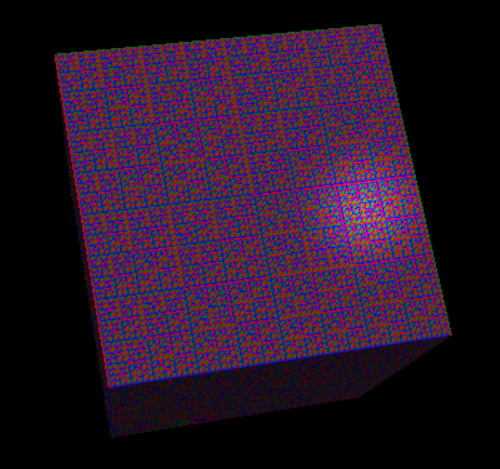
\includegraphics[width=0.73\textwidth]{images/light.png}
   \caption{Sześcian oświetlony według modelu Phonga}
   \label{lab:light}
\end{figure}
\begin{figure}[h!]
  \centering
    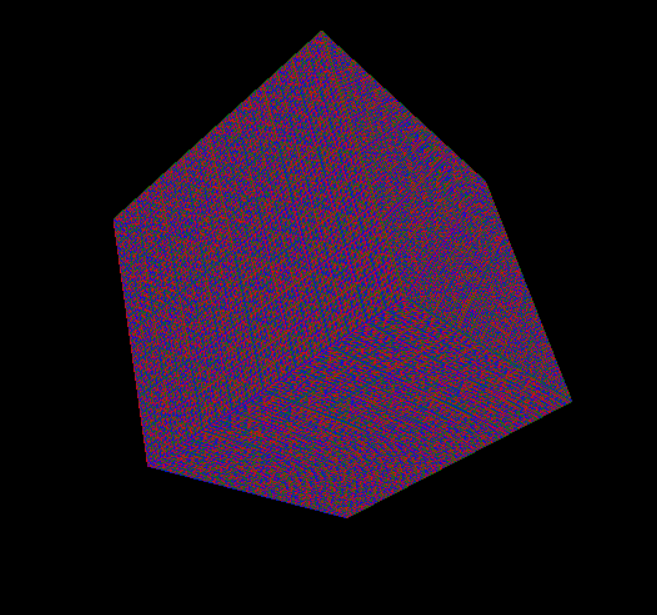
\includegraphics[width=0.73\textwidth]{images/nofrag.png}
   \caption{Sześcian z wykluczeniem oblicznień w shaderze fragmentów (brak oświetlenia)}
   \label{lab:nofrag}
\end{figure}
\begin{figure}[h!]
  \centering
    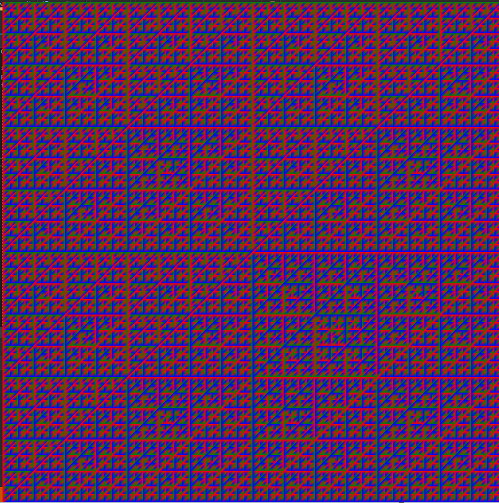
\includegraphics[width=0.60\textwidth]{images/noshad.png}
   \caption{Obraz wyrenderowany, gdy w shaderze wierzchołków nie wykonano przekształcenia MVP}
   \label{lab:noshad}
\end{figure}


Innym elementem, który zostanie poddany badaniom jest tryb \emph{line}/\emph{wireframe}. Jest to opcja, która pozwala na wyświetlanie jedynie siatki obiektu zamiast całych polygonów.  W praktyce tryb ten jest najczęściej stosowany podczas procesu budowy oprogramowania w celu szybszego i łatwiejszego lokalizowania i usuwania błędów. Na listingach \ref{lab:wireframecode} oraz \ref{lab:wireframecode2} przedstawiono jak należy skonfigurować potok graficzny, aby osiągnąć taki efekt. Na rysunku \ref{lab:wirepic} pokazano otrzymany efekt końcowy.\\

\begin{lstlisting}[caption={OpenGL – ustawienie trybu rysowania linii},captionpos=b,label={lab:wireframecode}]
gl.PolygonMode(SharpGL.Enumerations.FaceMode.Front,
SharpGL.Enumerations.PolygonMode.Lines);
\end{lstlisting}

\begin{lstlisting}[caption={DirectX – ustawienie trybu rysowania linii},captionpos=b,label={lab:wireframecode2}]
 _context.Rasterizer.State = new D3D11.RasterizerState(
 _device, new D3D11.RasterizerStateDescription
{
   FillMode = D3D11.FillMode.Wireframe
});

\end{lstlisting}

\begin{figure}[h!]
  \centering
    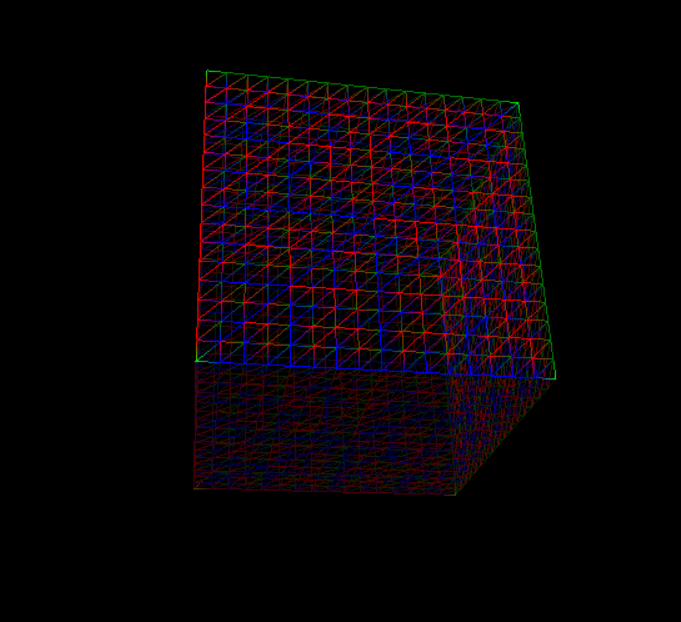
\includegraphics[width=0.73\textwidth]{images/wire.png}
   \caption{Sześcian w trybie wyświetlania linii}
   \label{lab:wirepic}
\end{figure}

Kolejnym elementem uwzględnionym podczas badań jest \emph{Face Culling}. Jest to proces, który powoduje, że rysowana jest tylko jedna strona polygonów. Ta opcja jest wykorzystywana w celach optymalizacyjnych, ponieważ często użytkownik widzi tylko jedną stronę polygonu. Tryb ten można włączyć w prosty sposób poprzez ustawienie odpowiednich flag (Listing \ref{lab:faceculling} oraz \ref{lab:faceculling2}). Należy, także zwrócić uwagę na to w jaki sposób jest określane, która powierzchnia jest przodem, a która tyłem. Jest to zdefiniowane poprzez kolejność wprowadzania wierzchołków polygonów, co pokazano na rysunku \ref{lab:wind} \cite{facecull}. Jeżeli nie wszystkie wierzchołki zostały wprowadzone w tej same kolejności, zastosowanie opcji \emph{Face Culling} może doprowadzić do efektu przedstawionego na rysunku \ref{lab:culpic}.

\begin{lstlisting}[caption={OpenGL – Face Culling},captionpos=b,label={lab:faceculling}]
gl.Enable(OpenGL.GL_CULL_FACE);
gl.CullFace(OpenGL.GL_BACK);

\end{lstlisting}
\begin{lstlisting}[caption={DirectX – Face Culling},captionpos=b,label={lab:faceculling2}]
_context.Rasterizer.State = new D3D11.RasterizerState(
_device, new D3D11.RasterizerStateDescription
{
   CullMode = D3D11.CullMode.Front,
   IsFrontCounterClockwise = false

});

\end{lstlisting}
\begin{figure}[h!]
  \centering
    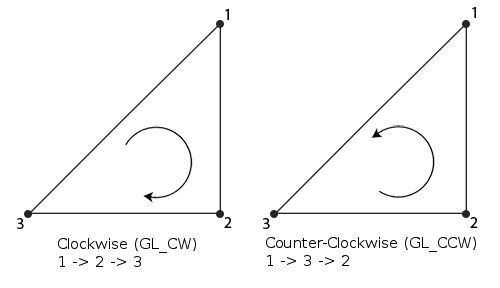
\includegraphics[width=0.44\textwidth]{images/Winding_order.png}
   \caption{Kierunek wprowadzania wierzchołków}
   Źródło: [https://www.khronos.org/opengl/wiki\_opengl/images/Winding\_order.png]
   \label{lab:wind}
\end{figure}
\begin{figure}[h!]
  \centering
    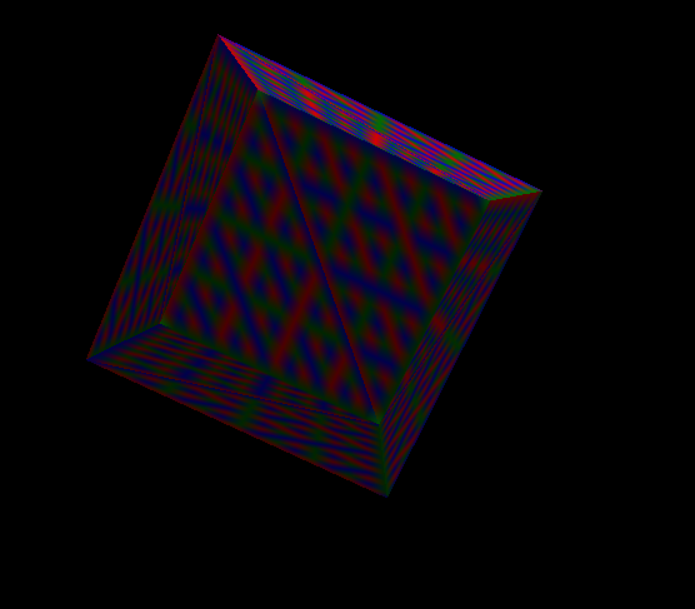
\includegraphics[width=0.5\textwidth]{images/cull.png}
   \caption{Face Culling zastosowany na sześcianie}
   \label{lab:culpic}
\end{figure}

Cześć badań wykonano przy użyciu programu \emph{TechPowerUp GPU-Z}, który pozwala mierzyć takie parametry jak zużycie pamięci VRAM, czy procentowe obciążenie GPU \cite{gpuz}. Interfejs programu przedstawiono na Rysunku \ref{lab:gpuz}.

\begin{figure}[h!]
  \centering
    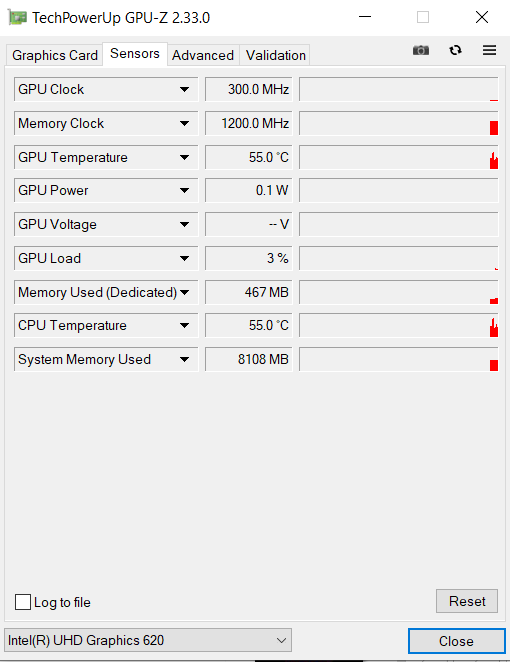
\includegraphics[width=0.4\textwidth]{images/gpuz.png}
   \caption{Interfejs programu GPU-Z}
   \label{lab:gpuz}
\end{figure}



\newpage


\section{Analiza wyników}

W tym rozdziale przedstawiono wyniki badań i dokonano analizy danych otrzymanych z wykonanych pomiarów. W kolejnych podrozdziałach znajdują się wyniki otrzymane dla badań różnych elementów API dla konfiguracji karta graficzna – interfejs. Na podstawie danych przedstawionych w formie wykresów lub tabel podjęto próbę wyciągnięcia wniosków i znalezienie zależności. W procesie formułowania wniosków wykorzystano również inne wykresy, nieprzedstawione w pracy jak np. odchylenie standardowe, wariancja czy współczynnik zmienności.


\subsection{Intensywne obliczenia w programach cieniujących}


Wykonane pomiary pokazują, że gdy w programach cieniujących wykonywana jest znaczna ilość obliczeń wydajność obu analizowanych interfejsów jest różna. Na rysunkach \ref{lab:11}, \ref{lab:12}, \ref{lab:13} przedstawiono wykresy liniowe, które obrazują różnice w~wydajności API dla różnych kart graficznych. Dla kart \emph{Nvidia GTX 770} oraz \emph{AMD Radeon 5700} czas renderowania sceny przy pomocy OpenGL jest niższy niż w przypadku DirectX, niezależnie od ilości wierzchołków. Dla karty graficznej firmy AMD duża różnica pojawia się skokowo po przekroczeniu liczby 8 milionów wierzchołków, a iloraz czasu dla obu API oscyluje wokół wartości 0,4–0,8 na korzyść OpenGL. Dla karty graficznej GTX 770 różnica w~wydajności narasta stopniowo wraz ze wzrostem liczby wierzchołków. Po przekroczeniu liczby 10 milionów wierzchołków iloraz utrzymuje się na poziomie 0,5 (Rysunek \ref{lab:13}). Natomiast dla zintegrowanej karty graficznej Intel UHD 620 interfejsem, który pozwala na szybsze renderowanie obrazu jest DirectX. Chodź różnica rośnie wraz ze wzrostem ilości wierzchołków, to iloraz spada. Dla 2 milionów wierzchołków iloraz ten wynosi 1,6, a~wraz ze zwiększaniem ilość wierzchołków obecnych na scenie spada do poziomu około 1,3 (Rysunek \ref{lab:14}). Współczynnik zmienności dla większości konfiguracji nie przekracza wartości 0,15. Konfiguracją, która cechuje się dużym odchyleniem standardowym i wariancją jest AMD Radeon 5700. Prawdopodobnie wynika to z faktu, że spośród badanych kart graficznych jest to karta najstarsza.



\begin{figure}[h!]
  \centering
    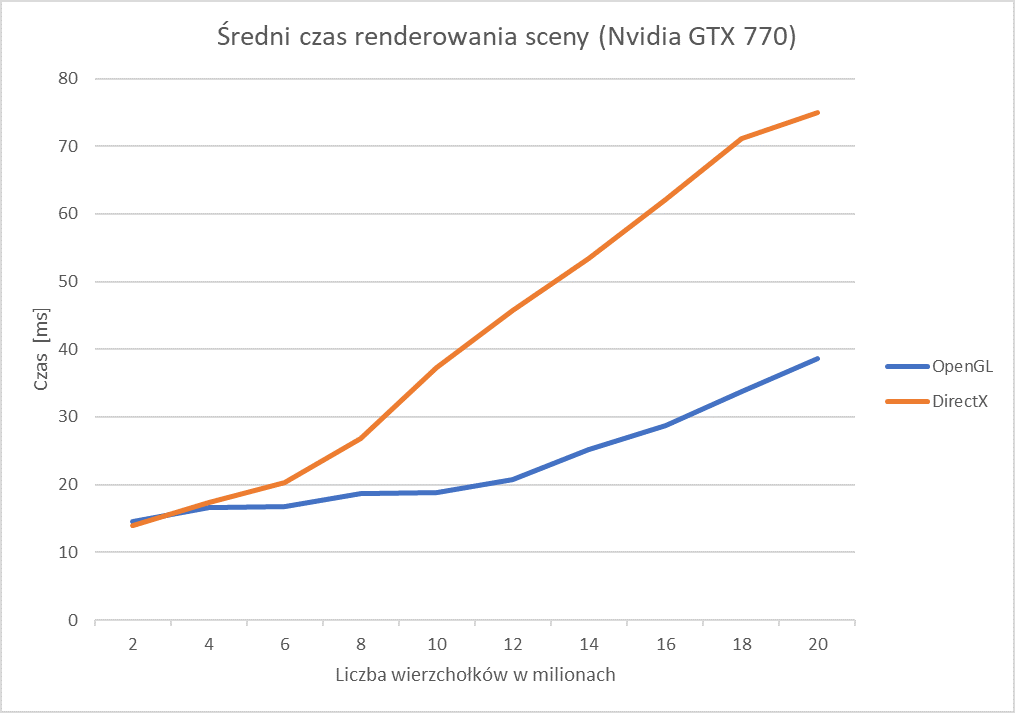
\includegraphics[width=0.9\textwidth]{images/shaderon/1.png}
   \caption{Średni czas renderowania sceny z intensywnymi obliczeniami w programach cieniujących dla karty Nvidia GTX 770}
   \label{lab:11}
\end{figure}
\newpage

\begin{figure}[h!]
  \centering
    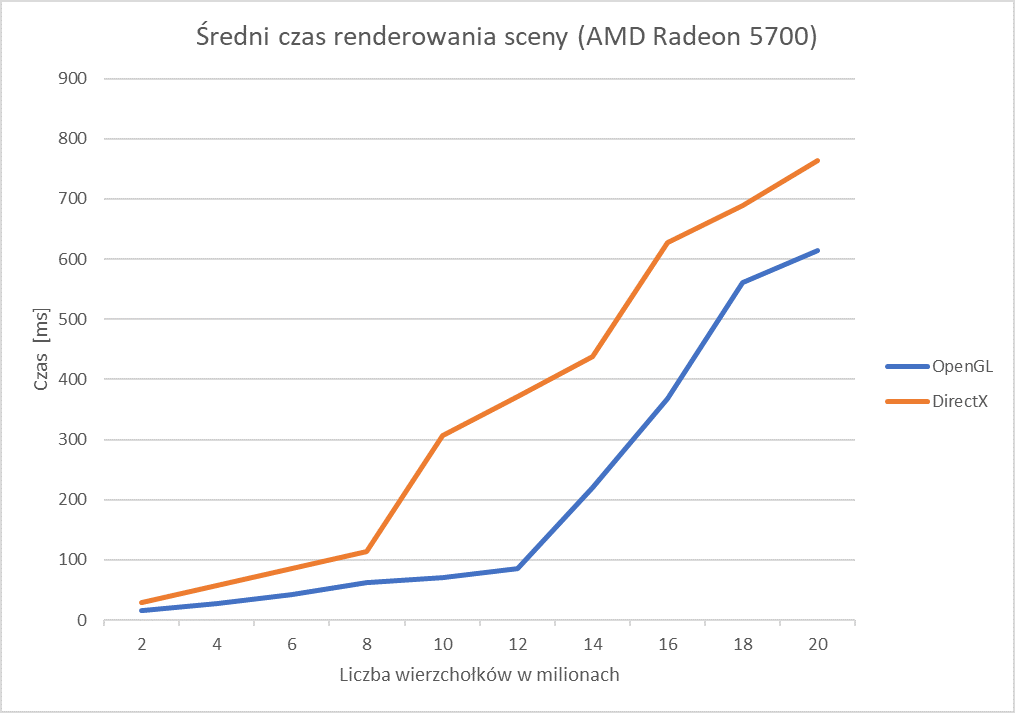
\includegraphics[width=0.9\textwidth]{images/shaderon/2.png}
   \caption{Średni czas renderowania sceny z intensywnymi obliczeniami w programach cieniujących dla karty AMD Radeon 5700}
   \label{lab:12}
\end{figure}
\bigbreak
\begin{figure}[h!]
  \centering
    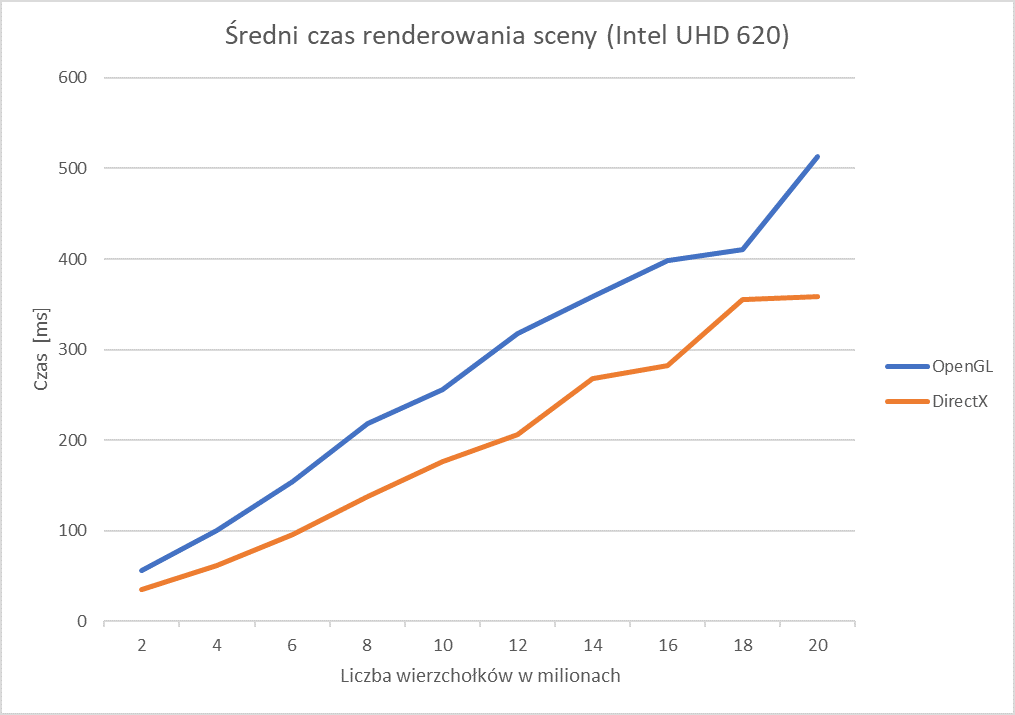
\includegraphics[width=0.9\textwidth]{images/shaderon/3.png}
   \caption{Średni czas renderowania sceny z intensywnymi obliczeniami w programach cieniujących dla karty Intel UHD 620}
   \label{lab:13}
\end{figure}
\newpage

\begin{figure}[h!]
  \centering
    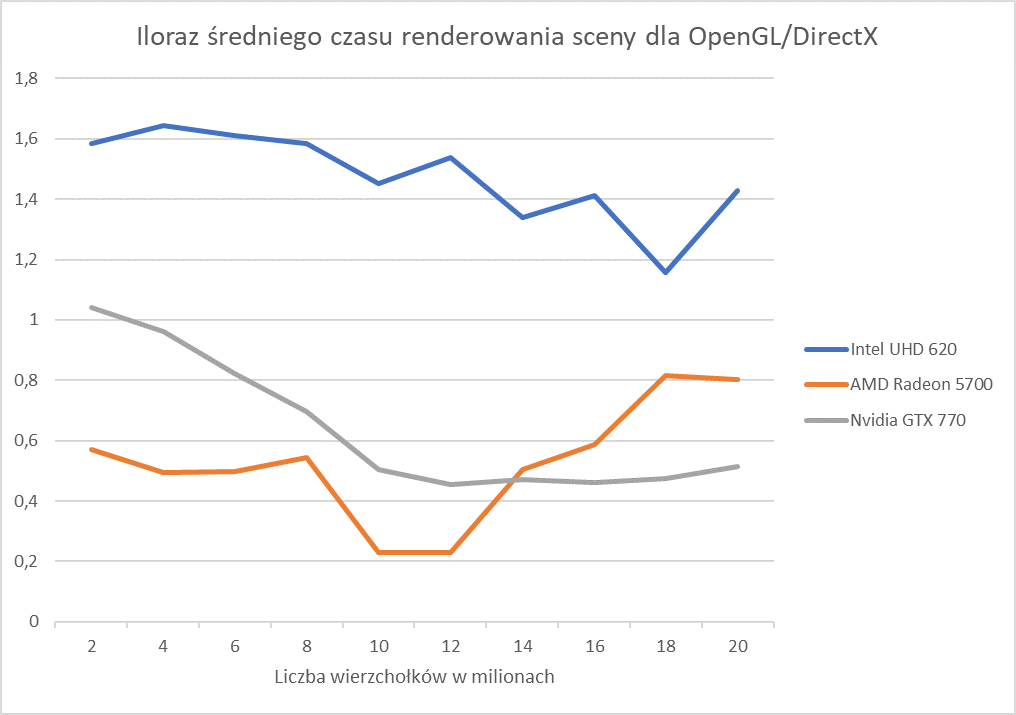
\includegraphics[width=0.9\textwidth]{images/shaderon/4.png}
   \caption{Iloraz średniego czasu renderowania sceny z intensywnymi obliczeniami w programach cieniujących dla OpenGL/DirectX}
   \label{lab:14}
\end{figure}

\subsection{Wyłączony moduł oświetlający}



Podczas tego badania sprawdzono jak ilość obliczeń w shaderze pikseli wpływa na czas renderowania sceny. Analiza wykresów pokazujących średni czas renderowania sceny (Rysunki \ref{lab:21}, \ref{lab:22}, \ref{lab:23}) pozwala na  formułowanie interesujących wniosków. Widać, że nadal dla kart AMD i Nvidia w ogólnym przypadku wydajniejszy jest interfejs OpenGL. Dla karty graficznej GTX 770 do poziomu 6 milionów scena jest szybciej renderowana przy pomocy API DirectX, a różnica pomiędzy interfejsami staje się istotna dopiero przy większej liczbie wierzchołków (co pokazano na Rysunku \ref{lab:24}). Odwrotna sytuacja zachodzi dla karty AMD, gdzie różnica pomiędzy wydajnością interfejsów jest większa niż w~poprzednim badaniu. Ciekawy jest również skokowy wzrost czasu potrzebnego na renderowanie sceny, który pojawia się przy 10 milionach wierzchołków dla DirectX oraz przy 14 dla OpenGL. Wyłączenie modułu oświetlenia sprawia, że wydajność obu interfejsów dla karty Intela zrównuje się. Wniosek tego badania jest taki, że obliczenia wykonywane w shaderze fragmentów/pikseli najmocniej wpływają na interfejs DirectX sprawiając, że sceny generowane z jego użyciem potrzebują odpowiednio więcej czasu niż dla OpenGL. Współczynnik zmienności dla większości konfiguracji utrzymuje się na poziomie 0,15. Wyjątkiem jest GTX 770 OpenGL, gdzie dla 4 i 6 milionów wierzchołków parametr ten osiąga wartość 0,35. Wariancja i odchylenie standardowe utrzymuje się na niskim poziomie dla API DirectX oraz wysokim dla OpenGL.

 \begin{figure}[h!]
  \centering
    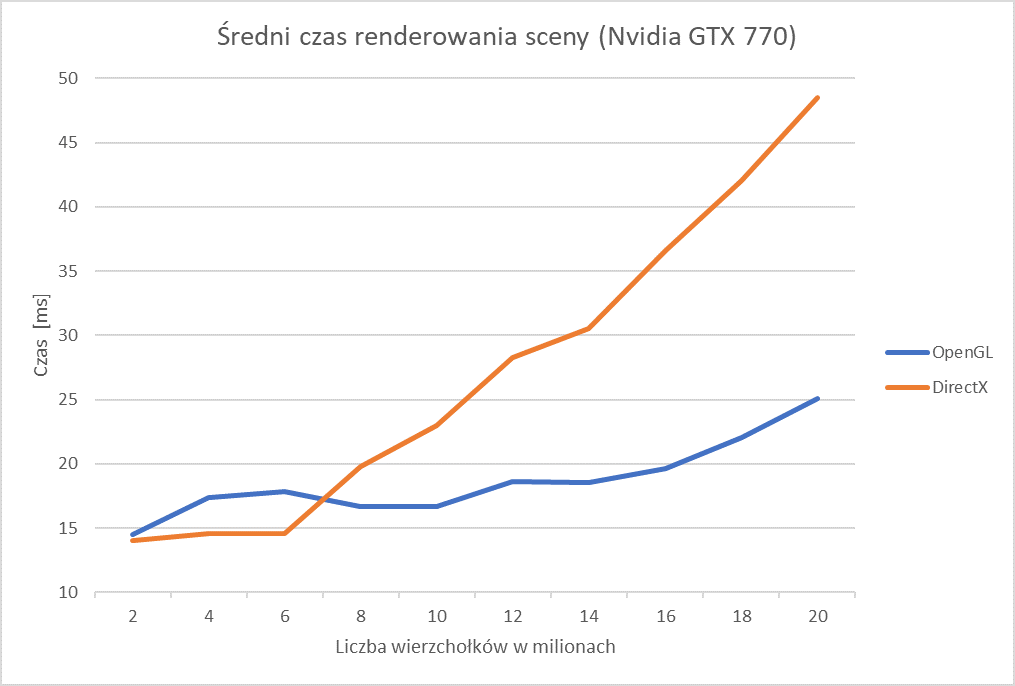
\includegraphics[width=0.9\textwidth]{images/fragoff/1.png}
   \caption{Średni czas renderowania sceny z wyłączonym oświetleniem dla karty Nvidia GTX 770}
   \label{lab:21}
\end{figure}
\newpage

\begin{figure}[h!]
  \centering
    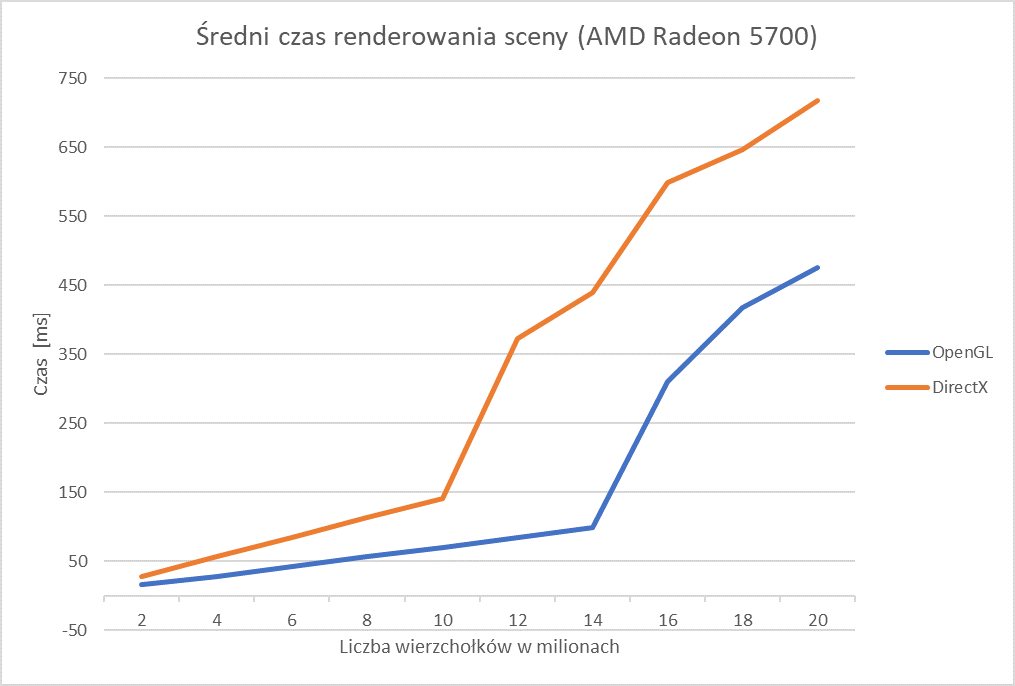
\includegraphics[width=0.9\textwidth]{images/fragoff/2.png}
   \caption{Średni czas renderowania sceny z wyłączonym oświetleniem dla karty AMD Radeon 5700}
   \label{lab:22}
\end{figure}
\bigbreak
\begin{figure}[h!]
  \centering
    \includegraphics[width=0.9\textwidth]{images/fragoff/3.png}
   \caption{Średni czas renderowania sceny z wyłączonym oświetleniem dla karty Intel UHD 620}
   \label{lab:23}
\end{figure}
\newpage

\begin{figure}[h!]
  \centering
    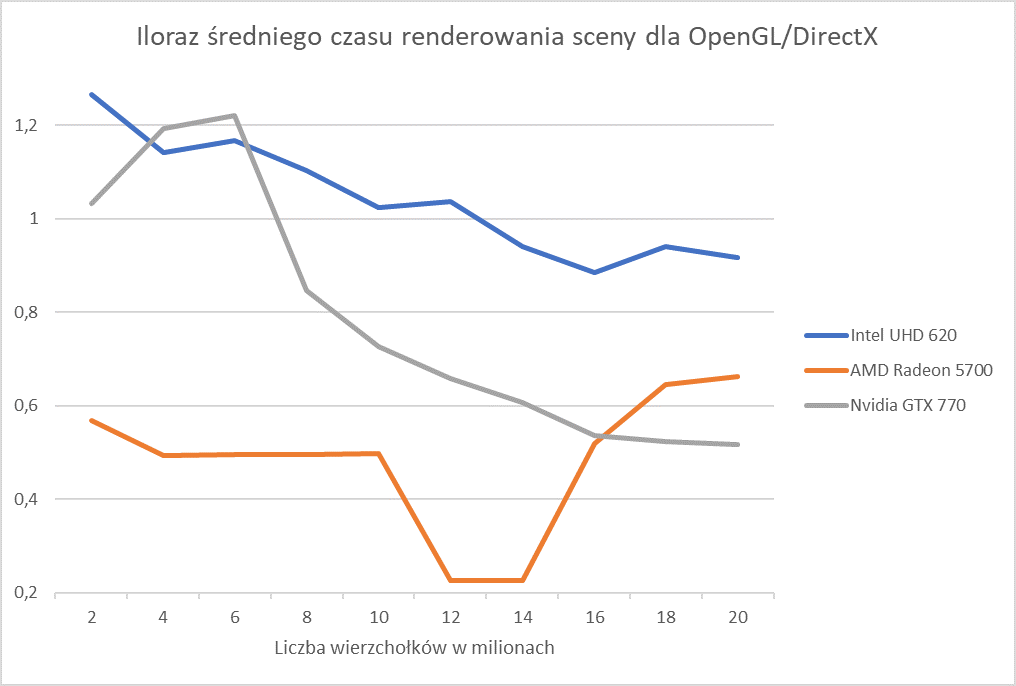
\includegraphics[width=0.9\textwidth]{images/fragoff/4.png}
   \caption{Iloraz średniego czasu renderowania sceny z wyłączonym oświetleniem dla OpenGL/DirectX}
   \label{lab:24}
\end{figure}

\subsection{Minimalizacja obliczeń wykonywanych w programach cieniujących}

W tym badaniu oprócz wyłączenia modułu oświetlenia w shaderze pikseli, usunięto również obliczenia wykonywane w shaderze wierzchołków. Otrzymane wyniki są niemal identyczne do tych wykonanych w punkcie 4.3.2. Zarówno średni czas renderowania sceny jak i parametry statystyczne utrzymują się na podobnym poziomie niezależnie od zawartości programu cieniującego wierzchołków. Wynika to z faktu, że obliczenia, które zostały zredukowane na potrzeby wykonania tego badania, czyli przekształcenia MVP są tak tanie obliczeniowo, że nie mają wpływu na sposób działania API. Przekształcenie to jest prostym mnożeniem macierzy i w porównaniu do obliczenia oświetlenia piksela jest pod względem wydajnościowym nieistotne. W celu lepszego zbadania tego elementu shader wierzchołków powinien zawierać obliczenia dużo bardziej kosztowne obliczeniowo.

\begin{figure}[h!]
  \centering
    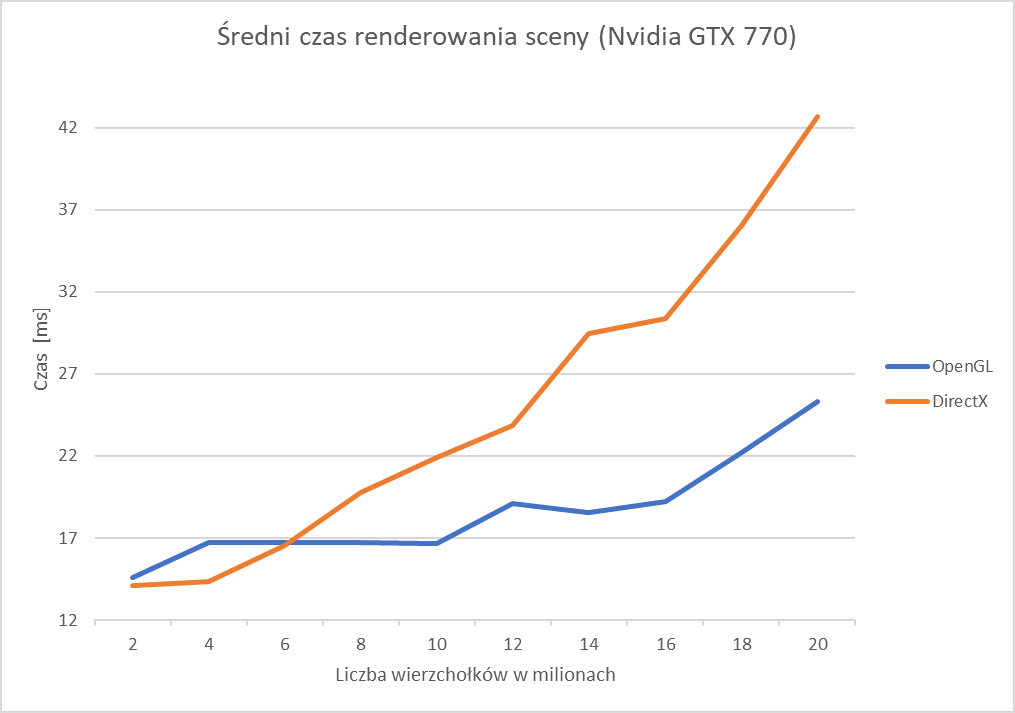
\includegraphics[width=0.9\textwidth]{images/shaderoff/1.png}
   \caption{Średni czas renderowania sceny z minimalizacją obliczeń wykonywanych w programach cieniujących dla karty Nvidia GTX 770}
   \label{lab:31}
\end{figure}
\newpage

\begin{figure}[h!]
  \centering
    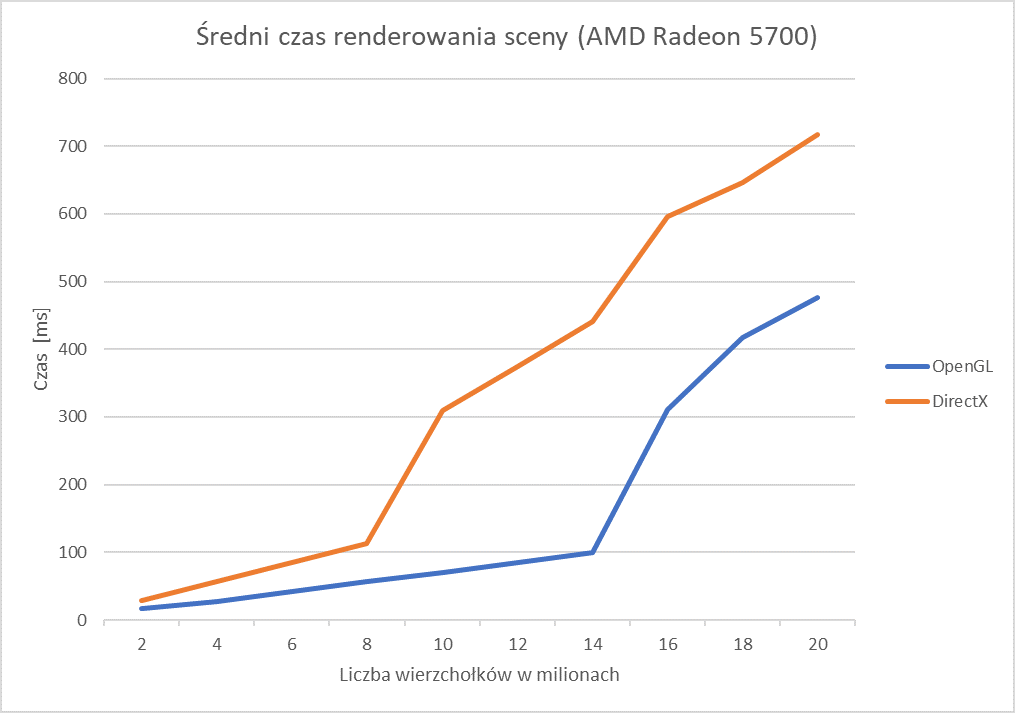
\includegraphics[width=0.9\textwidth]{images/shaderoff/2.png}
   \caption{Średni czas renderowania sceny z minimalizacją obliczeń wykonywanych w programach cieniujących dla karty AMD Radeon 5700}
   \label{lab:32}
\end{figure}
\bigbreak
\begin{figure}[h!]
  \centering
    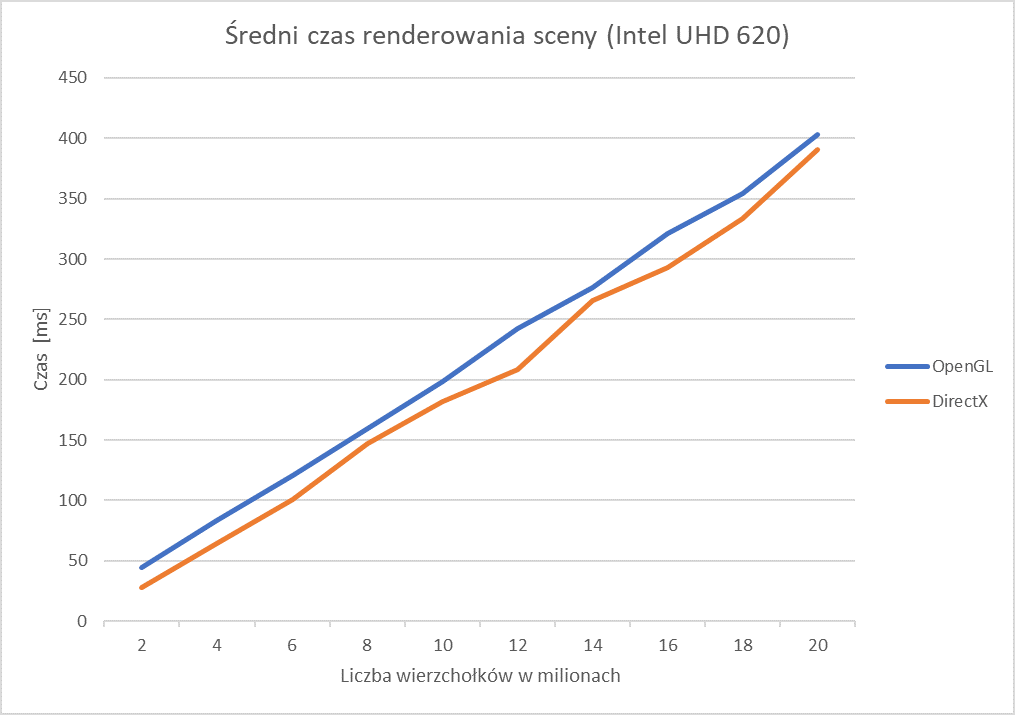
\includegraphics[width=0.9\textwidth]{images/shaderoff/3.png}
   \caption{Średni czas renderowania sceny z minimalizacją obliczeń wykonywanych w programach cieniujących dla karty Intel UHD 620}
   \label{lab:33}
\end{figure}
\newpage

\begin{figure}[h!]
  \centering
    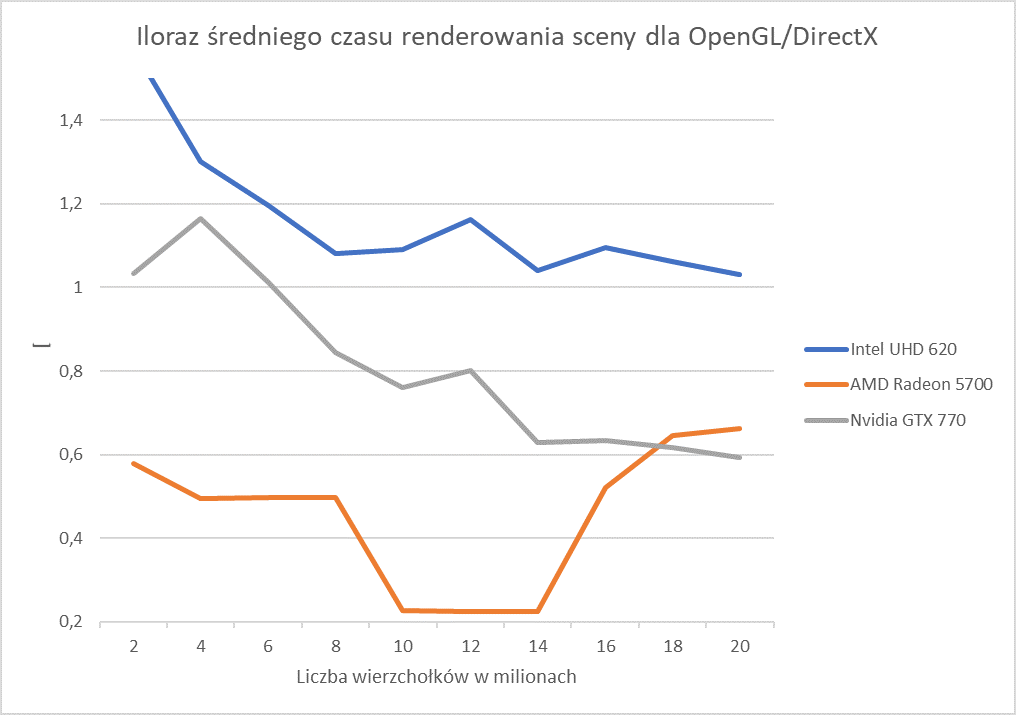
\includegraphics[width=0.9\textwidth]{images/shaderoff/4.png}
   \caption{Iloraz średniego czasu renderowania sceny z minimalizacją obliczeń wykonywanych w programach cieniujących dla OpenGL/DirectX}
   \label{lab:34}
\end{figure}

\subsection{Tryb usuwania niewidocznych powierzchni}

Tryb usuwania niewidocznych krawędzi powstał w celu zredukowania ilość wykonywanych obliczeń na procesorze karty graficznej, a co za tym idzie zmniejszenie czasu potrzebnego na wyrenderowanie sceny. Na Rysunkach \ref{lab:41}, \ref{lab:42}, \ref{lab:43} przedstawiono wykresy średniego czasu potrzebne na wygenerowanie pojedynczej klatki. Po ich porównaniu do wykresów z punktu 4.3.1 można zauważyć, że kształt i trend wykresów dla takich samych kart jest niemal identyczny. Oznacza to, że wpływ tego trybu na wydajność jest taki sam niezależnie od używanej karty graficznej. Ponad to Rysuneki \ref{lab:44} i \ref{lab:14} zawierające iloraz średniego czasu pokazują, że różnice w wydajności obu interfejsów są stałe. Według wyników pomiarów tryb ten pozwala na zmniejszenie czasu potrzebnego na wyrenderownie sceny o około 10\% dla kart Intel UHD 620 i Nvidia GTX 770. W przypadku karty AMD Radeon 5700 tryb ten jest skuteczniejszy i pozwala na redukcje czasu o około 20\%. Różnica jest tym bardziej widoczne im więcej wierzchołków jest obecnych na scenie. Wariancja oraz odchylenie standardowe – podobnie jest we wcześniejszych rozdziałach – dla większości konfiguracji utrzymuje się na niskim poziomie. Większe wartości tych parametrów statystycznych pojawiają się dla starszych kart, które posiadają mniejszą ilość pamięci VRAM. Procesor musi co jakiś czas dosyłać karcie graficznej resztę danych, ponieważ na wszystkie jednocześnie brakuje miejsca. 

\begin{figure}[h!]
  \centering
    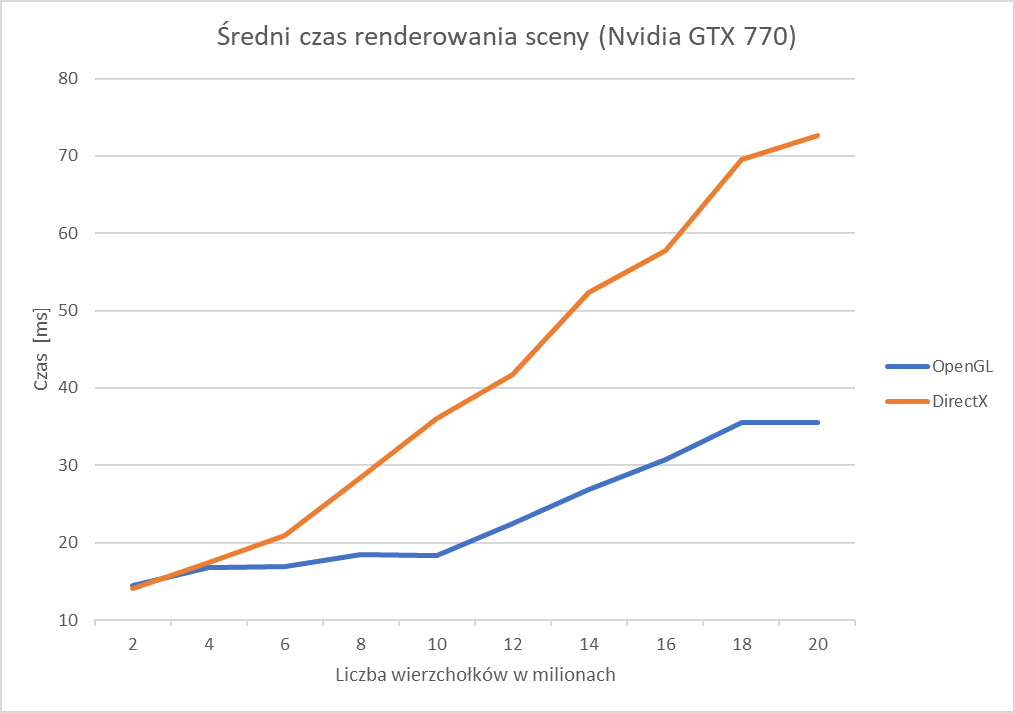
\includegraphics[width=0.9\textwidth]{images/cull/1.png}
   \caption{Średni czas renderowania sceny z włączonym trybem usuwania niewidocznych powierzchni dla karty Nvidia GTX 770}
   \label{lab:41}
\end{figure}
\newpage

\begin{figure}[h!]
  \centering
    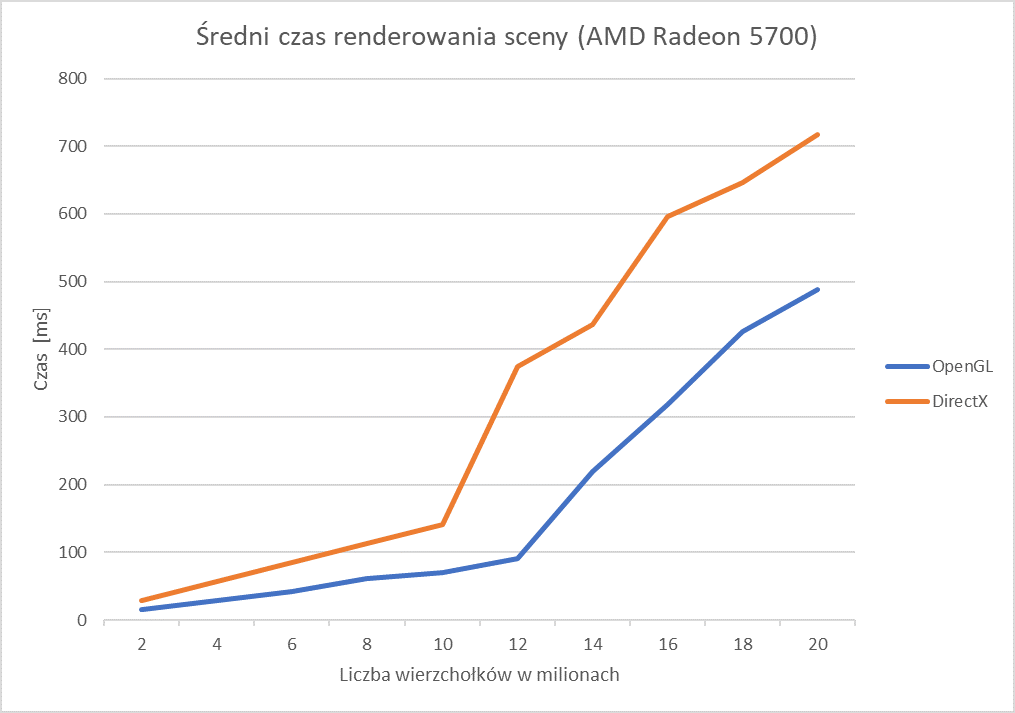
\includegraphics[width=0.9\textwidth]{images/cull/2.png}
   \caption{Średni czas renderowania sceny z włączonym trybem usuwania niewidocznych powierzchni dla karty AMD Radeon 5700}
   \label{lab:42}
\end{figure}
\bigbreak
\begin{figure}[h!]
  \centering
    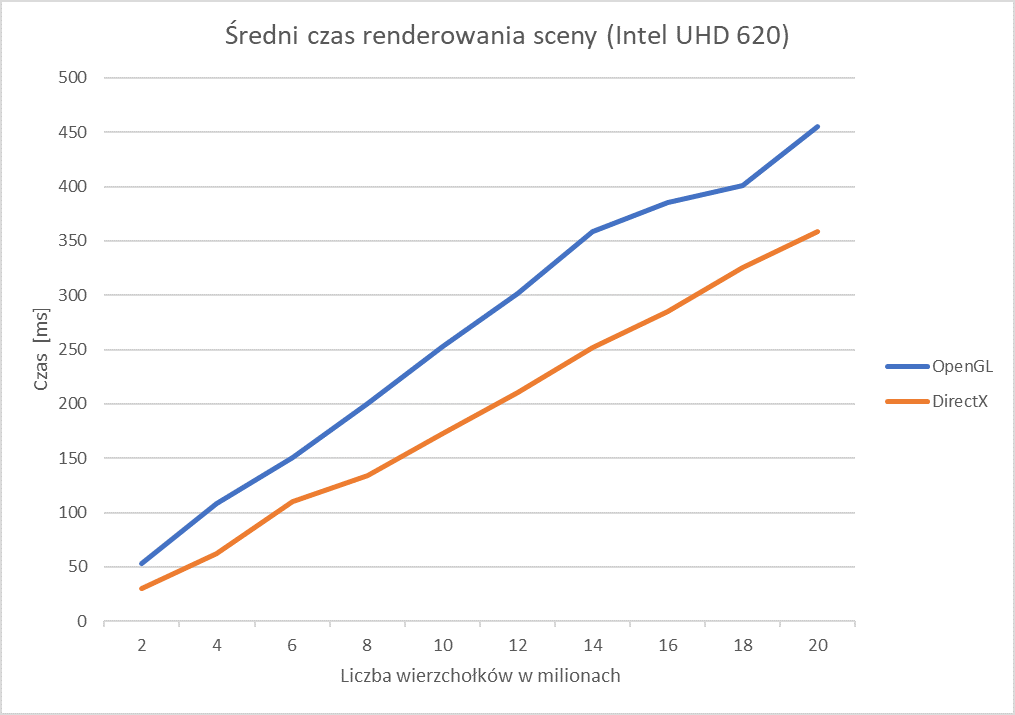
\includegraphics[width=0.9\textwidth]{images/cull/3.png}
   \caption{Średni czas renderowania sceny z włączonym trybem usuwania niewidocznych powierzchni dla karty Intel UHD 620}
   \label{lab:43}
\end{figure}
\newpage

\begin{figure}[h!]
  \centering
    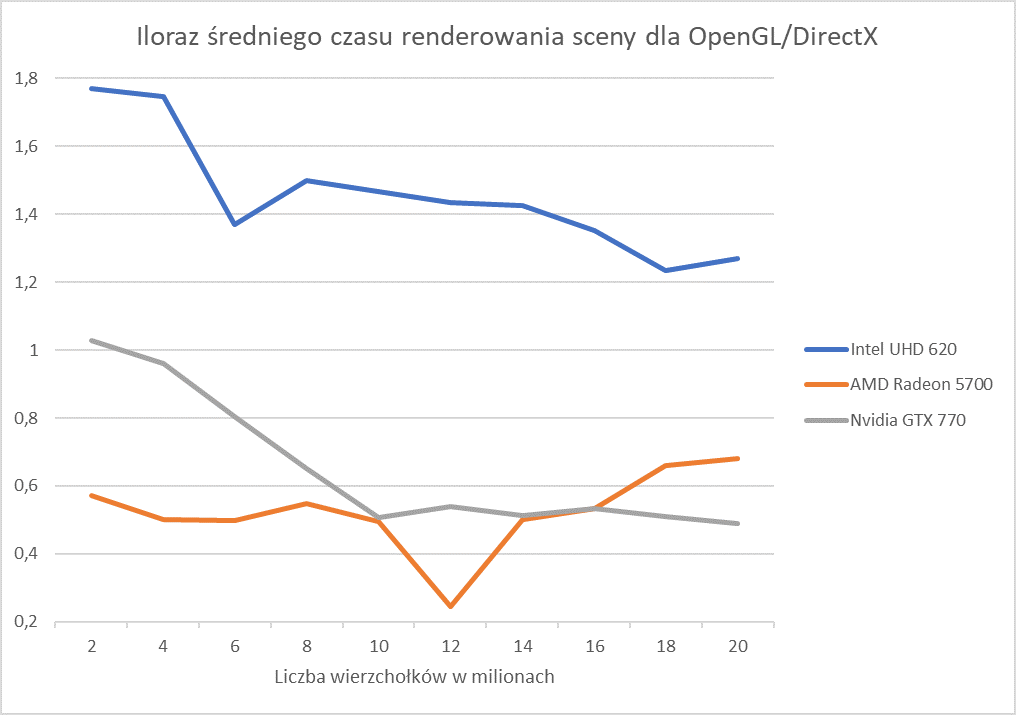
\includegraphics[width=0.9\textwidth]{images/cull/4.png}
   \caption{Iloraz średniego czasu renderowania sceny z włączonym trybem usuwania niewidocznych powierzchni dla OpenGL/DirectX}
   \label{lab:44}
\end{figure}

\subsection{Tryb rysowania linii}

Włączenie trybu rysowania linii spowodowało wzrost średniego czasu renderowania sceny, co jest szczególnie widoczne dla karty Nvidia GTX 770 (wzrost o 375\%). Wzrost ten dotyczył obu API, a z wykresów \ref{lab:51}, \ref{lab:52}, \ref{lab:53} i \ref{lab:54} wynika, że rodzaj użytego interfejsu ma mały wpływ na tę zmianę. W tym trybie nadal dla kart AMD oraz Nvidia lepszą wydajność osiągana jest przy pomocy OpenGL (średni czas renderowania sceny niższy o około 50\%), natomiast DirectX lepiej sprawdza się dla kart Intel (średni czas renderowania sceny niższy o około 40–70\%).


\begin{figure}[h!]
  \centering
    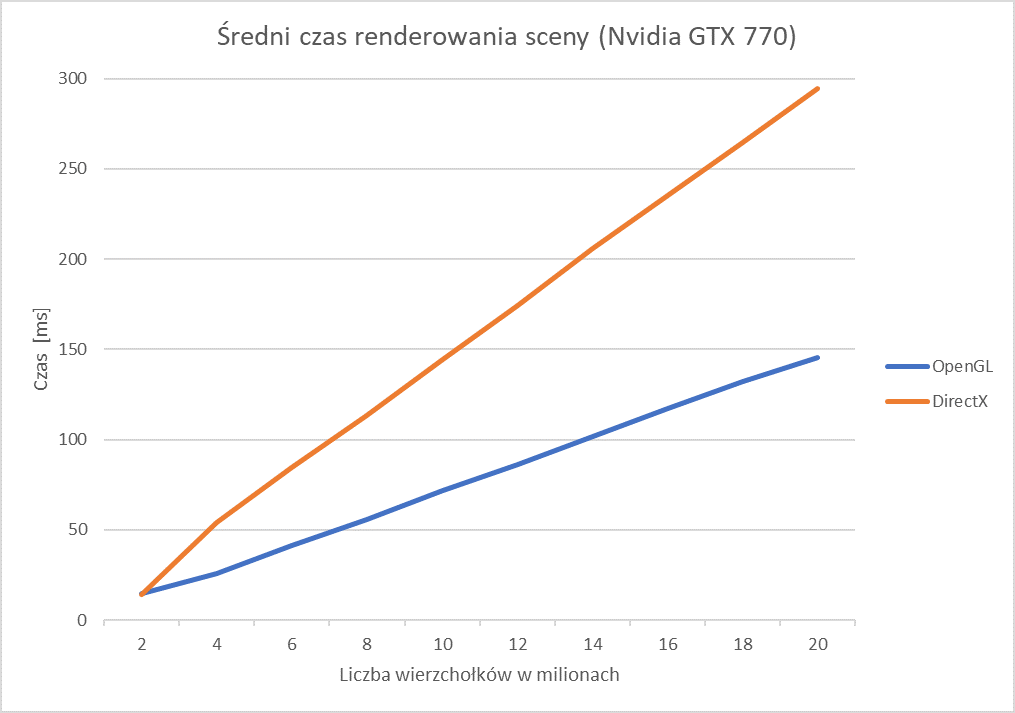
\includegraphics[width=0.9\textwidth]{images/wire/1.png}
   \caption{Średni czas renderowania sceny z włączonym trybem rysowania linii dla karty Nvidia GTX 770}
   \label{lab:51}
\end{figure}
\newpage

\begin{figure}[h!]
  \centering
    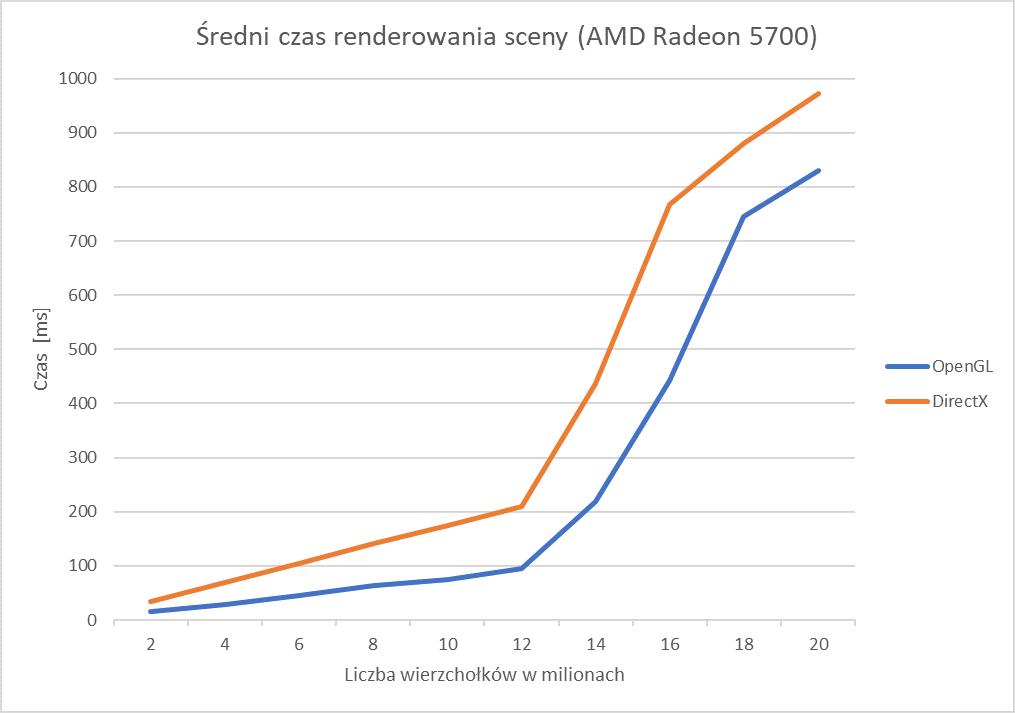
\includegraphics[width=0.9\textwidth]{images/wire/2.png}
   \caption{Średni czas renderowania sceny z włączonym trybem rysowania linii dla karty AMD Radeon 5700}
   \label{lab:52}
\end{figure}
\bigbreak
\begin{figure}[h!]
  \centering
    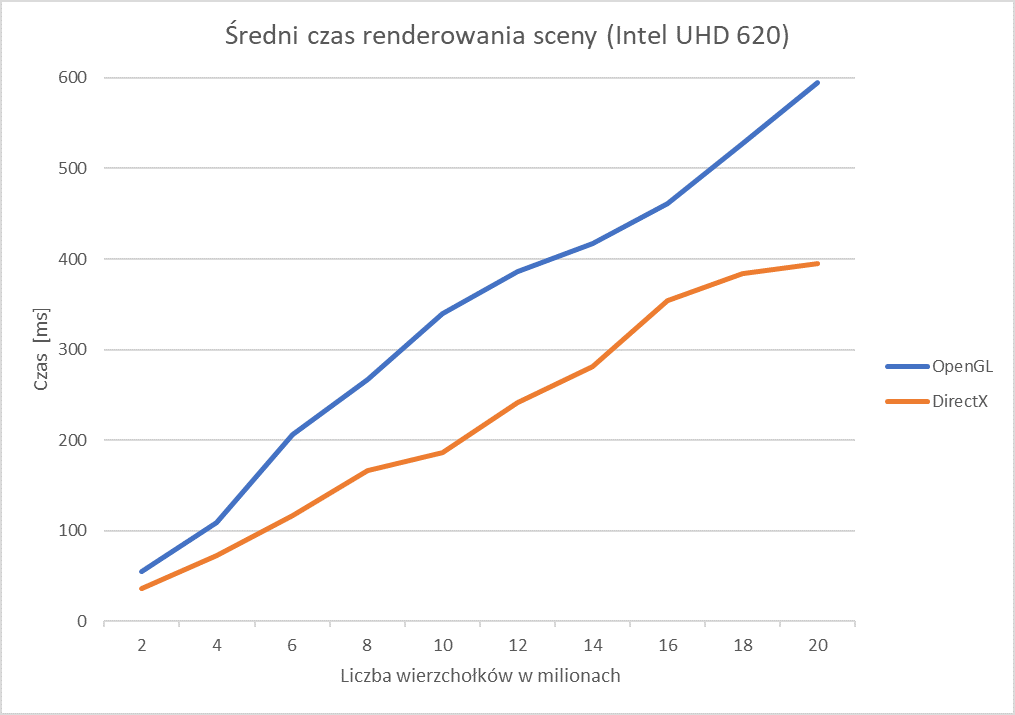
\includegraphics[width=0.9\textwidth]{images/wire/3.png}
   \caption{Średni czas renderowania sceny z włączonym trybem rysowania linii dla karty Intel UHD 620}
   \label{lab:53}
\end{figure}
\newpage

\begin{figure}[h!]
  \centering
    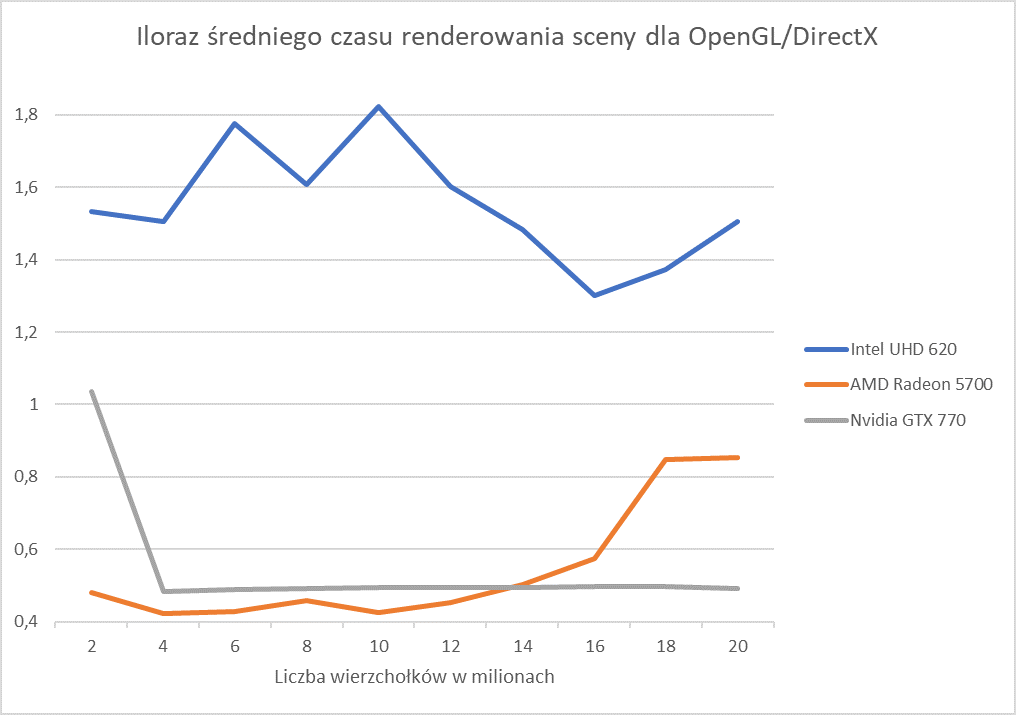
\includegraphics[width=0.9\textwidth]{images/wire/4.png}
   \caption{Iloraz średniego czasu renderowania sceny z włączonym trybem rysowania linii dla OpenGL/DirectX}
   \label{lab:54}
\end{figure}
\bigbreak

\subsection{Przesyłanie danych do pamięci VRAM}


W tym rozdziale badaniom poddano czas wysyłania danych w formie informacji o~wierzchołkach do pamięci karty graficznej. Wykresy \ref{lab:61}, \ref{lab:62}, \ref{lab:63} przedstawiają średni czas wysyłania określonej liczby wierzchołków. Dla karty graficznej Nvidia GTX 770 czas ten rośnie liniowo względem liczby wierzchołków – w przybliżeniu 25 milisekund na każde 2~miliony wierzchołków. Różnice w wydajności interfejsów znajdują się w granicach błędu statystycznego, można więc wyciągnąć wniosek, że działają tak samo wydajnie. Ponad to wysyłanie danych na tej karcie odbywa się około 4 razy szybciej niż dla pozostałych (dla OpenGL). Różnice w wydajności pomiędzy API są natomiast widoczne dla kart AMD Radeon 5700 oraz Intel UHD 620. Dla obu tych kart DirectX niezależnie od ilości wierzchołków potrzebuje około 4 razy mniej czasu na ich wysłanie. Prawdopodobnie wynika to z niewielkiej dostępnej pamięci VRAM tych kart. Ciekawy jest fakt, że DirectX osiągnął taki sam wynik niezależnie od karty graficznej Największą wariancją i odchyleniem standardowych cechują się pomiary wykonane dla karty Nvidia GTX 770.

\begin{figure}[h!]
  \centering
    \includegraphics[width=0.9\textwidth]{images/data/1.png}
   \caption{Średni czas przesyłania danych do karty Nvidia GTX 770}
   \label{lab:61}
\end{figure}
\newpage

\begin{figure}[h!]
  \centering
    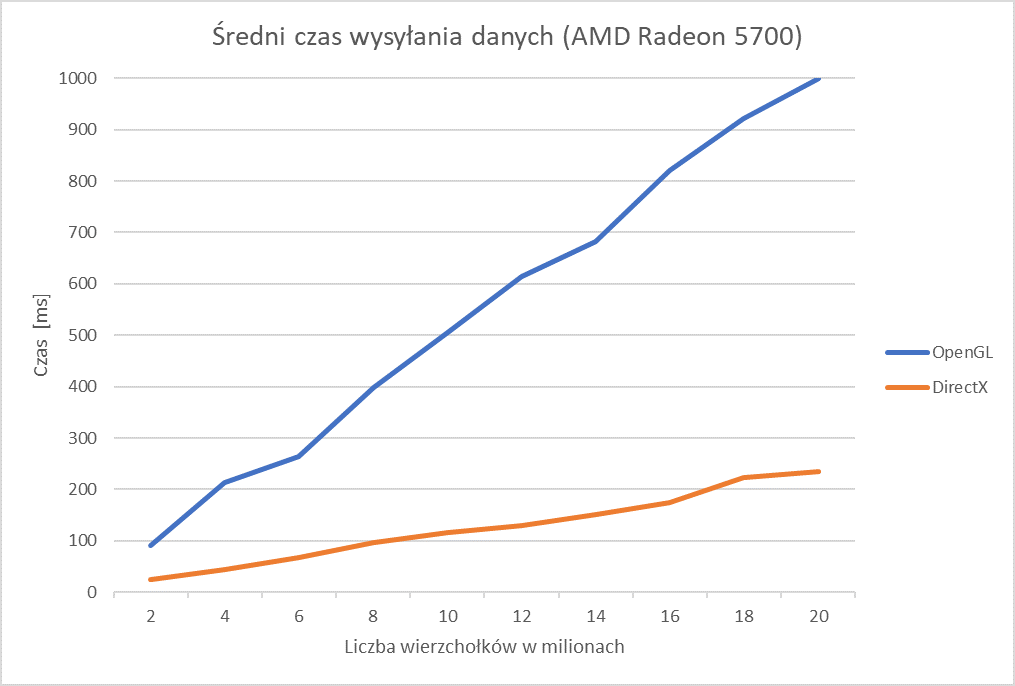
\includegraphics[width=0.9\textwidth]{images/data/2.png}
   \caption{Średni czas przesyłania danych do karty AMD Radeon 5700}
   \label{lab:62}
\end{figure}
\bigbreak
\begin{figure}[h!]
  \centering
    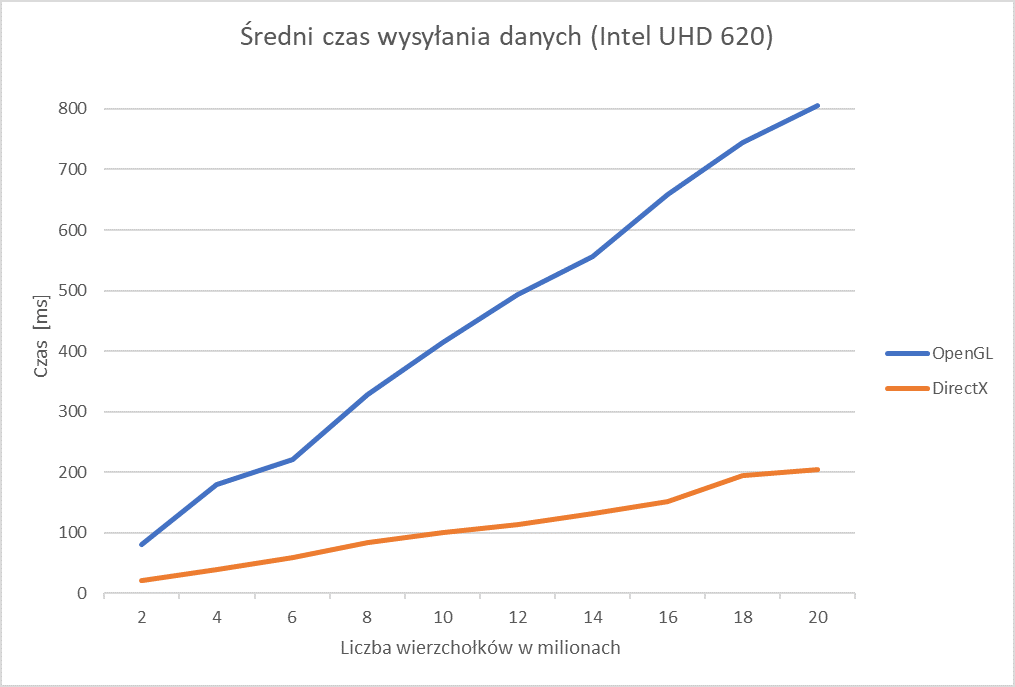
\includegraphics[width=0.9\textwidth]{images/data/3.png}
   \caption{Średni przesyłania danych do karty Intel UHD 620}
   \label{lab:63}
\end{figure}
\newpage

\begin{figure}[h!]
  \centering
    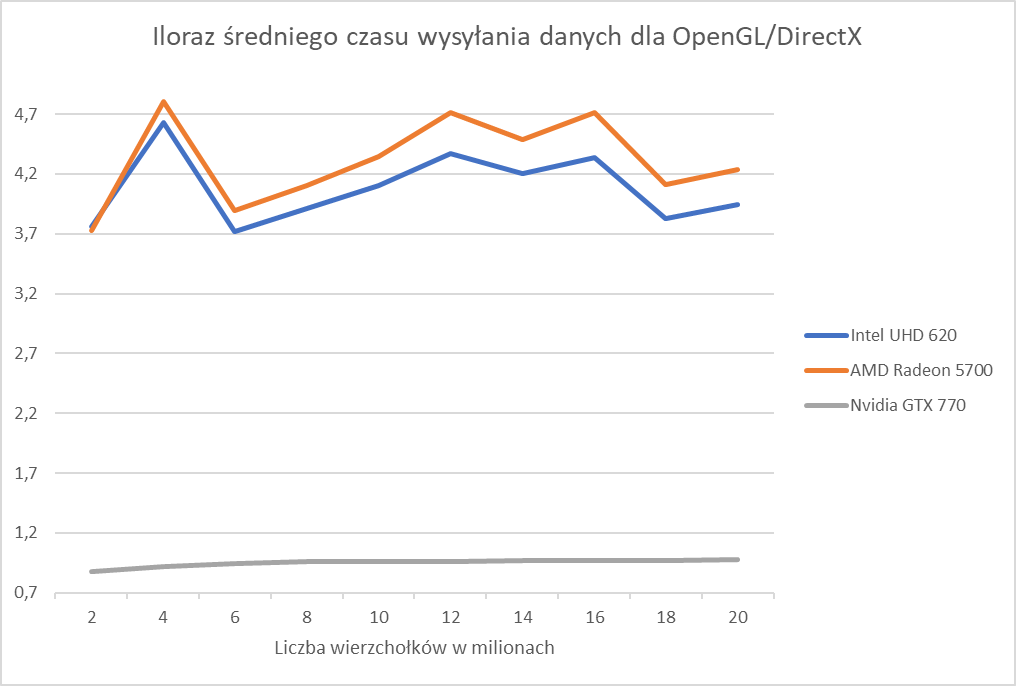
\includegraphics[width=0.9\textwidth]{images/data/4.png}
   \caption{Iloraz średniego czasu przesyłania danych dla OpenGL/DirectX}
   \label{lab:64}
\end{figure}

\subsection{Obciążenie procesora graficznego}

Oprócz badań czasu wykonano również pomiar obciążenia procesora graficznego. 
Wartość średnia pochodzi ze 100 pomiarów wykonanych co sekundę. Dla karty Nvidia jest znacząca różnica w obciążeniu GPU pomiędzy interfejsami. Przy użyciu DirectX obciążenie utrzymuje się na poziomie 100\% niezależnie od liczby wierzchołków, a dla OpenGL wartość ta początkowo wynosi około 50\% (dla 2 milionów wierzchołków) by wzrastać i~ostatecznie pozostać na poziomie 100\% dla 10 milionów wierzchołków i więcej. Zupełnie inny trend wskazują wyniki otrzymane z kart AMD. Oba interfejsu obciążają GPU w~takim samym stopniu – około 93\% do 8 milionów wierzchołków oraz 100\% ponad tą wartość. Jednak najciekawszych wyników dostarcza karta Intel UHD 620. Obciążenie przy użyciu OpenGL wraz ze wzrostem liczby wierzchołków wzrasta z poziomu 85\% do 97\%.  Dla DirectX średnie obciążenie procesora spada wraz ze wzrostem ilości wierzchołków. Po przyjrzeniu się danym nieuśrednionym można zauważyć, że pojawiają się naprzemiennie wartości 0\% oraz 100\%. Wynika to z tego, że API nie jest w stanie wystarczająco szybko dostarczyć tak dużej liczby dany do GPU, więc procesor czeka i zmniejsza częstotliwość.


\begin{figure}[h!]
  \centering
    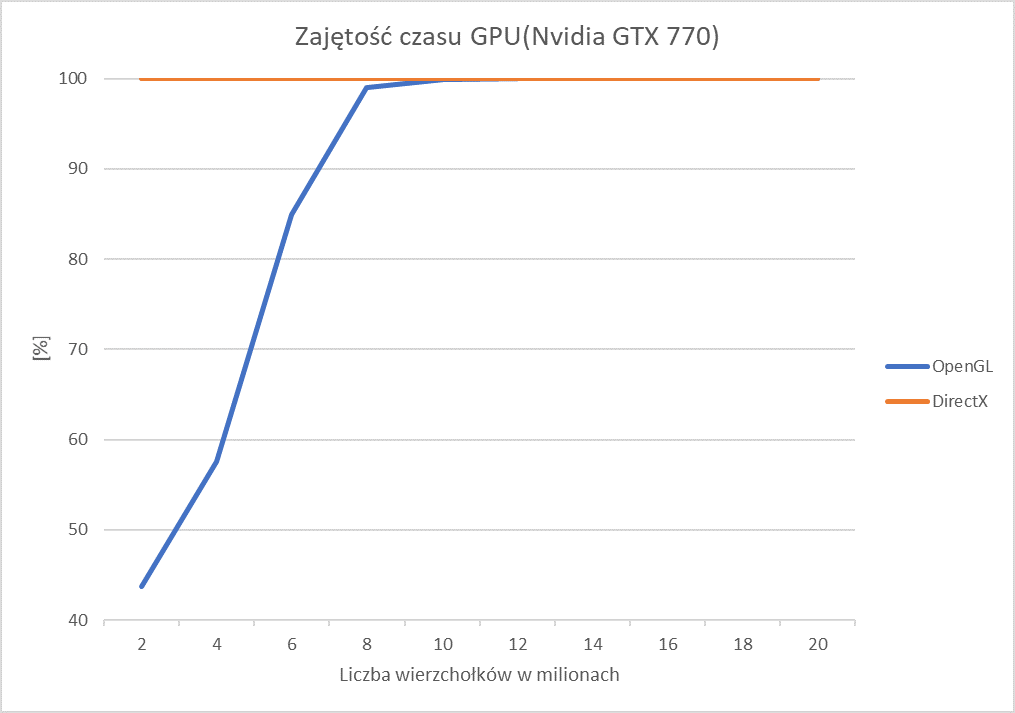
\includegraphics[width=0.9\textwidth]{images/gpu/1.png}
   \caption{Średnie obciążenie procesora graficznego (Nvidia GTX 770)}
   \label{lab:71}
\end{figure}
\newpage

\begin{figure}[h!]
  \centering
    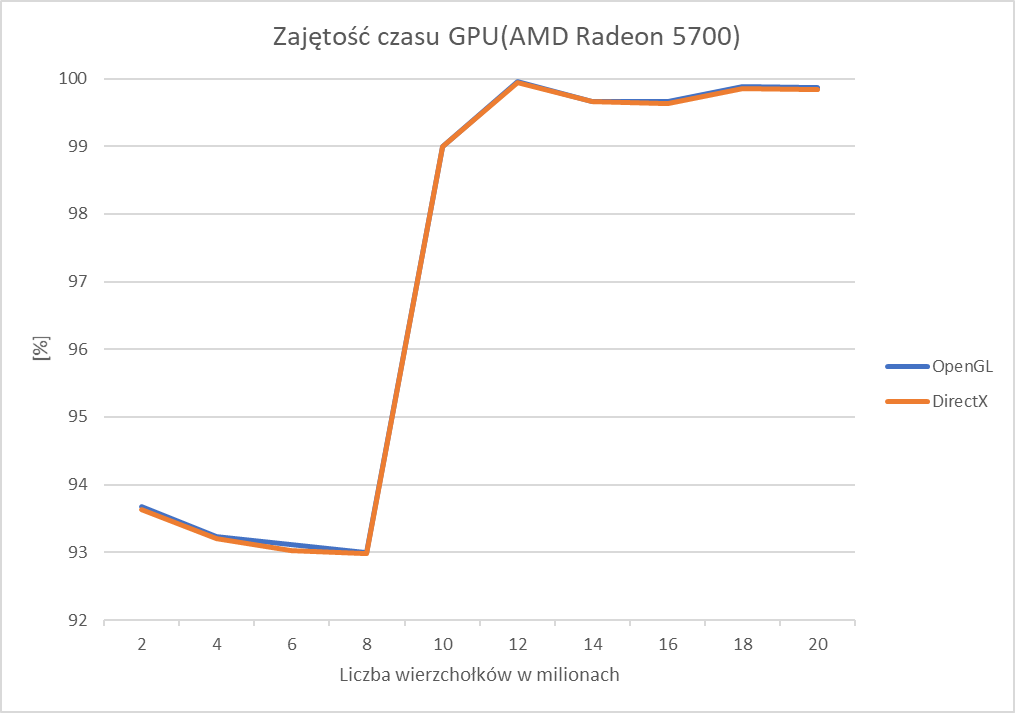
\includegraphics[width=0.9\textwidth]{images/gpu/2.png}
   \caption{Średnie obciążenie procesora graficznego (AMD Radeon 5700)}
   \label{lab:72}
\end{figure}
\bigbreak
\begin{figure}[h!]
  \centering
    \includegraphics[width=0.95\textwidth]{images/gpu/3.png}
   \caption{Średnie obciążenie procesora graficznego (Intel UHD 620)}
   \label{lab:73}
\end{figure}
\begin{figure}[h!]
  \centering
    \includegraphics[width=0.95\textwidth]{images/gpu/4.png}
   \caption{Iloraz średniego obciążenia procesora graficznego dla OpenGL/DirectX)}
   \label{lab:73}
\end{figure}

\newpage

\subsection{Zajętość pamięci VRAM}

Na Rysunkach \ref{lab:81}, \ref{lab:82}, \ref{lab:83} przedstawiono średnią ilość zajętości pamięci VRAM dla danej liczby wierzchołków. Dla karty Nvidia ilość ta różni się w zależności od API o~wartość około 400MB dla 2 milionów wierzchołków. Wraz z zwiększaniem ilość wierzchołków wartości dla obu interfejsów dążą do liczby 1600MB. Dla karty AMD nie zauważono znaczącej różnicy w ilości zajętej pamięci przez analizowane API. Dla 2 milionów wierzchołków zajmują one około 300MB a dla 20 1100MB. Różnice w zajętości pamięci pomiędzy interfejsami można zauważyć dla karty firmy Intel. Niezależnie od ilości wierzchołków dane przesłane za pomocą API OpenGL zajmują około 10\% pamięci mniej. Odchylenie standardowe oraz wariancja jest dla karty Intel stosunkowo większe niż dla innych kart. Wynika to, z~niewielkiej ilości pamięci VRAM dostępnej w tej karcie graficznej. API musi często przesyłać dane pomiędzy pamięcią RAM i~VRAM co wprowadza wariancję. Z tego samego powodu dane przesyłane za pomocą OpenGL zajmują mniej miejsca. W tym interfejsie zarządzanie pamięcią znajduje się w sterowniku graficznym, a ten lepiej zarządza pamięcią i procesem przesyłania danych pomiędzy pamięcią RAM i~VRAM.




\begin{figure}[h!]
  \centering
    \includegraphics[width=0.9\textwidth]{images/vram/1.png}
   \caption{Średnia ilość zajętej pamięcia VRAM (Nvidia GTX 770)}
   \label{lab:81}
\end{figure}
\newpage

\begin{figure}[h!]
  \centering
    \includegraphics[width=0.9\textwidth]{images/vram/2.png}
   \caption{Średnia ilość zajętej pamięcia VRAM (AMD Radeon 5700)}
   \label{lab:82}
\end{figure}
\bigbreak
\begin{figure}[h!]
  \centering
    \includegraphics[width=0.95\textwidth]{images/vram/3.png}
   \caption{Średnia ilość zajętej pamięcia VRAM (Intel UHD 620)}
   \label{lab:83}
\end{figure}

\begin{figure}[h!]
  \centering
    \includegraphics[width=0.80\textwidth]{images/vram/4.png}
   \caption{Iloraz średniej ilośći zajętej pamięci VRAM OpenGL/DirectX}
   \label{lab:84}
\end{figure}
\newpage

\subsection{Kompilowanie programów cieniujących}

Ostatnim z badanych elementów jest czas kompilowania programów cieniujących.Jest to proces, który przetwarza kod źródłowy programów cieniujących w ciąg bajtów, który steruje potokiem graficznym. W tabeli \ref{lab:shadertable} znajduje się podsumowanie wykonanych pomiarów. Najbardziej istotna jest pierwsza kolumna zawierająca średnią ze 100 wykonanych pomiarów czasu dla każdej z konfiguracji. Jak można zauważyć czas ten jest niezależny od użytego API i wynosi około 13 ms dla stacji z kartami AMD oraz Intel i około 11,5 ms dla stacji z kartą Nvidia. Mniejszy czas dla tej karty wynika z faktu, że komputer w nią wyposażony posiada silniejsze podzespoły. Pozostałe parametry informują o stosunkowo niskim odchyleniu standardowym oraz wariancji.

\begin{table}[!h]

    \centering 
    \caption{Wyniki pomiary czasu kompilowania programów cieniujących}
    		\label{lab:shadertable}
    \vspace{2mm} 
\begin{tabular}{|p{2.5cm}|p{2cm}|p{3cm}|p{3cm}|p{2cm}|p{1.5cm}|}
\hline

\textbf{Konfiguracja} &	\textbf{Średni czas [ms]}	&\textbf{Odchylenie standardowe}&\textbf{Współczynnik zmienności}&\textbf{Wariancja}&\textbf{Iloraz}\\ \hline

Intel UHD 620 OpenGL &12,72
&1,17
&0,09
&1,38
&1,03
\\ \hline

Intel UHD 620 DirectX &12,45
&0,93
&0,07
&0,86
&0,97
\\ \hline

AMD Radeon 5700 OpenGL &12,78

&1,31

&0,10

&1,73

&0,99


\\ \hline

AMD Radeon 5700 DirectX &12,82
&1,25
&0,09
&1,57
&1,01

\\ \hline

Nvidia GTX 770 OpenGL &11,56

&1,10

&0,09

&1,22

&1,02

\\ \hline

Nvidia GTX 770 DirectX &11,43

&1,03

&0,09

&1,06

&0,98
\\ \hline

\end{tabular}
\end{table}
\newpage
\subsection{Podsumowanie}

Przeprowadzone badania wskazują, że nie jest możliwe jednoznaczne wskazanie, które API jest wydajniejsze. W zależności od użytej karty graficznej jedno API górowało nad drugim. Dla układów Nvidia GTX 770 oraz AMD Radeon 5700 zmierzony czas renderowania klatki był prawie zawsze mniejszy dla API OpenGL. W zależności od rodzaju wykonanego testu, ta przewaga rosła lub malała, ale zawsze była zauważalna.\\

Odmienne wyniki otrzymano dla karty zintegrowanej Intel UHD 620. Dla każdego testu dotyczącego pomiaru czasu generowania klatki DirectX osiągnął lepszy wynik dla tej karty. Zauważono również, że intensywne obliczenia wykonywane w~shaderze pikseli mają większy wpływ na wzrost czasu niż te wykonywane w shaderze fragmentów. Niestety nie udało się osiągnąć wartościowych wyników dotyczących wpływu intensywności obliczeń w~shaderze wierzchołków na wydajność. Obliczenia, które wykorzystano do obciążenia karty graficznej, czyli mnożenie macierzy, okazały się zbyt mało kosztowne obliczeniowo i~miały znikomy wpływ na działanie programu.\\

Interesujące dane otrzymano przy pomiarze czasu wysyłania danych do karty graficznej. Wynika z nich, że wybór API nie ma żadnego wpływu na czas dla karty Nvidia, lecz dla pozostałych układów występuje duża przewaga API DirectX. Dzięki tej informacji użytkownicy tych kart, mogą być skłonni do wyboru jednego API nad drugim. Pozostałe zmierzone parametry takie jak obciążenie procesora graficznego czy ilość zajętej pamięci również nie dają jednoznacznej odpowiedzi, które API jest wydajniejsze.

\chapter{Zakończenie}


Zaprezentowana praca poruszyła zagadnienia z dziedziny, która ma szerokie zastosowanie w wielu branżach. Przedstawiono najważniejsze mechanizmy i cechy charakterystyczne dwóch obecnie najpopularniejszych API graficznych – DirectX i OpenGL. Opisano szereg różnych elementów poczynając od historii i genezy, a kończąc na szczegółach w sposobie działania potoku graficznego. Następnie zestawiono oba interfejsy i wskazano najważniejsze podobieństwa i różnice między nimi.\\

Wszystkie cele w pracy zostały zrealizowane, lecz dla części z nich nie udało się wykonać pewnych elementów. Wykonano przegląd literatury oraz zbudowano narzędzie badawcze – silnik graficzny. Zawarto w nim wszystkie założone funkcjonalności poza teksturowaniem. Zostały zaplanowane badania oraz przygotowano przykłady testowe. Na ich podstawie oraz z wykorzystaniem silnika graficznego wykonano pomiary wydajności. Rezultaty poddano analizie, lecz z powodu zbyt dużych różnic w metodzie wykonywanie pomiarów nie wykonano porównania ich z wynikami literaturowymi.\\

Pierwszym wnioskiem z przeprowadzonych badań jest to, że wydajność API graficznych jest zagadnieniem złożonym, zaś wynik jest zależny od wielu czynników. W związku z tym, próby wyciągania wniosków o charakterze ogólnym są bezzasadne lub wymagają przeprowadzenia badań o innej skali lub charakterze. W celu otrzymania bardziej jednoznacznego wyniku należałoby przeprowadzić badania dla większej liczby kart graficznych, a same pomiary wykonać dla pojedynczych operacji na GPU z większą dokładnością pomiaru. Niemniej, na podstawie uzyskanych wyników można przeprowadzić szereg wniosków szczegółowych, zachodzących w specyficznych warunkach. Przede wszystkim dla kart dedykowanych (AMD, Nvidia) OpenGL osiąga niższy czas renderowania sceny niż DirectX. Dla karty zintegrowanej (Intel) przewaga jednego API nad drugim jest zależne od intensywności obliczeń w programie cieniującym. Kolejnym wnioskiem jest fakt, że czas przesyłania danych do pamięci VRAM za pomocą DirectX rośnie liniowo wraz ze wzrostem ilości danych, niezależnie od użytej karty graficznej. Przesyłanie danych za pomocą API OpenGL trwało dłużej i w dużym stopniu zależało od układu graficznego. Ostatni ważny wniosek dotyczy trybu usuwanie niewidocznych powierzchni. Nie zauważono istotnych różnic we wzroście wydajności pomiędzy API przy zastosowaniu tego trybu.\\

Wykazano, że istnieją różnice w wydajności omawianych interfejsów, lecz są one zależne od wielu czynników, a wybór jednego API nad drugim powinien być oparty o postawione wymagania dla konkretnego zastosowania. Dzięki wynikom przedstawionym w pracy możliwe jest celniejsze dopasowanie API do konkretnego celu.


\addcontentsline{toc}{chapter}{\bibname}

\begin{thebibliography}{9}
\bibitem{OpenGLHistory}\emph{History of OpenGL}, \url{https://www.khronos.org/opengl/wiki/History_of_OpenGL}, [dostęp dnia 15.08.2020 r.].
\bibitem{OpenGLExtensions}\emph{OpenGL Extension}, \url{https://www.khronos.org/opengl/wiki/OpenGL_Extension}, [dostęp dnia 15.08.2020 r.].
\bibitem{kiciak}
  Przemysław Kiciak,
  \emph{OpenGL i GLSL (krótki kurs)}, 2017/2018.
\bibitem{Rendering_Pipeline_Overview}\emph{Rendering Pipeline Overview}, \url{https://www.khronos.org/opengl/wiki/Rendering_Pipeline_Overview}, [dostęp dnia 15.08.2020 r.].
\bibitem{OpenGLAttrib}\emph{OpenGL Documentation glVertexAttribPointer}, \url{https://www.khronos.org/registry/OpenGL-Refpages/gl4/html/glVertexAttribPointer.xhtml}, [dostęp dnia 15.08.2020 r.].
\bibitem{VertexSpecification}\emph{OpenGL Vertex Specification}, \url{https://www.khronos.org/opengl/wiki/Vertex_Specification}, [dostęp dnia 15.08.2020 r.].
\bibitem{OpenGLVertexShader}\emph{OpenGL Vertex Shader}, \url{https://www.khronos.org/opengl/wiki/Vertex_Shader}, [dostęp dnia 15.08.2020 r.].
\bibitem{OpenGLPrimitives}Paul Martz, \emph{OpenGL Primitives}, ISBN: 0321336798, EAN: 2147483647, 2007, Strona: 123.
\bibitem{the-history-of-directx}\emph{History of DirectX}, \url{https://www.codingunit.com/the-history-of-directx}, [dostęp dnia 15.08.2020 r.].
\bibitem{DirectXVersions}Gabriel Torres, \emph{DirectX Versions}, \url{https://www.hardwaresecrets.com/directx-versions/}, [dostęp dnia 15.08.2020 r.].
\bibitem{DirectXDocumentation}DirectX Microsoft Documentation, \url{https://docs.microsoft.com/en-us/windows/win32/direct3d11}, [dostęp dnia 15.08.2020 r.].
\bibitem{directxHLSL}Craig Peeper, Jason L. Mitchell, \emph{Introduction to the DirectX® 9High Level Shading Language}, Microsoft Corporation, 2003.
\bibitem{DirectXTesselation}Hilbert Hagedoorn, \emph{Radeon HD 5830 review - DirectX 11 - Hardware Tessellation}, \url{https://www.guru3d.com/articles-pages/radeon-hd-5830-review,6.html}, [dostęp dnia 15.08.2020 r.].
\bibitem{Billboarding}\emph{Billboarding (Geometry Shader)}, \url{https://www.braynzarsoft.net/viewtutorial/q16390-36-billboarding-geometry-shader}, [dostęp dnia 15.08.2020 r.].
\bibitem{DirectXRaster}Nick Evanson, \emph{How 3D Game Rendering Works, A Deeper Dive: Rasterization and Ray Tracing}, \url{https://www.techspot.com/article/1888-how-to-3d-rendering-rasterization-ray-tracing/}, [dostęp dnia 15.08.2020 r.].
\bibitem{DirectXdepth}\emph{Basics of 2D depth testing}, \url{https://badlogicgames.com/forum/viewtopic.php?f=11&t=9300}, [dostęp dnia 15.08.2020 r.].
\bibitem{wine}\emph{Wine HQ}, \url{https://www.winehq.org/}, [dostęp dnia 15.08.2020 r.].
\bibitem{compar}Richard Dazeley, \emph{3D APIs in Interactive Real-Time Systems:Comparison of OpenGL, Direct3D and Java3D}, University of Tasmania, 2000.
\bibitem{valley}\emph{Unigine Valley}, \url{https://benchmark.unigine.com/valley}, [dostęp dnia 15.08.2020 r.].
\bibitem{book}Kevin Hawkins, Dave Astle, \emph{OpenGL Game Programming}, Cengage Learning PTR, 2002.

\bibitem{lit1}Torbjörn Sörman, \emph{Comparison of Technologies for General-Purpose Computing on Graphics Processing Units}, Linköping University, 2016.

\bibitem{lit2}Anthony Lovesey, \emph{A Comparison of Real Time Graphical Shading Languages}, University of New Brunswick, 2005.

\bibitem{lit3}Joseph Shiraef, \emph{An Exploratory Study Of High Performance Graphics Application Programming Interfaces}, The University of Tennessee at Chattanooga, Chattanooga, Tennessee, 2016.

\bibitem{lit4}Jerzy Dąbkowski, \emph{Porównanie Wydajności Języków Cieniowania CG i HLSL}, Instytut Teleinformatyki, Politechnika Krakowska, 2010.
\bibitem{sharpdx}\emph{SharpDX}, \url{http://sharpdx.org/}, [dostęp dnia 15.08.2020 r.].
\bibitem{facecull}\emph{Face Culling}, \url{https://www.khronos.org/opengl/wiki/Face_Culling}, [dostęp dnia 15.08.2020 r.].\\
\bibitem{gpuz}\emph{TechPowerUp GPU-Z}, \url{https://www.techpowerup.com/}, [dostęp dnia 15.08.2020 r.].\\


\end{thebibliography}
\appendix
\chapter{Opis zawartości płyty CD}
Do pracy załączono płytę CD zawierającą:
\begin{itemize}
\item pracę dyplomową w wersji elektronicznej,
\item kod źródłowy autorskiego silnika graficznego,
\item wyniki pomiarów w formie pliku arkusza kalkulacyjnego.
\end{itemize}
\end{document}
